\chapter[The Environmental Dependence of Low-$z$ $\rm Ly\alpha$ Absorption]{The Environmental Dependence of Low-$z$ $\rm Ly\alpha$ Absorption}
%THE ENVIRONMENTAL DEPENDENCE OF LOW-$z$ LY$\alpha$ ABSORPTION]{THE ENVIRONMENTAL DEPENDENCE OF LOW-$z$ LY$\alpha$ ABSORPTION} 
\label{chap:chap5}

% Leave space between title and quote or publication note.  This has often been
% 10cm for a quote and 8 cm for a reference, but this is really up to you.
%\vspace{8cm}

\vfill

\begin{flushright}
  \fixspacing % Single spacing
  \textit{To be submitted to the \emph{Astrophysical Journal}} \\
%  \vspace{1ex} Tofflemire, et al.\ 2017, \apj, 835, 8
\end{flushright}

\vspace*{1in} % Leave a 1-in space at the bottom.

\cleardoublepage

\begin{chabstract}

We present the results of a large-scale study of the Ly$\alpha$-probed CGM of nearby galaxies. We have identified 1135 Ly$\alpha$ absorbers in the redshift range $0 \leq z \leq 0.033$ in the spectra of 264 background QSOs, and correlated their positions with the surrounding galaxy environment. This has produced a sample of 216 individual Ly$\alpha$ component-galaxy pairs, representing the largest-to-date dataset of its kind. By employing the likelihood-based matching scheme of \cite{french2017}, we quantify the absorber-galaxy spacial correlation and identify 4 distinct absorber sub-samples based on their relative isolation from surrounding galaxies. We find that absorber equivalent width (EW) and Doppler-$b$ parameter are enhanced with increasing proximity to galaxies, with the isolated absorber EW distribution differing from that of galaxy-associated absorbers at a $>5 \sigma$ level. Confirming the findings of \cite{french2017}, we find an overabundance of detections at high galaxy inclination ($\sim 4.5 \sigma$). We also report the first significant detection of an azimuth dependence for $\rm Ly\alpha$ absorption, with both an enhanced detection fraction and an overabundance of absorption near the major and minor axes ($\sim 3.3 \sigma$). Taken together these results suggest a picture in which weak $\rm Ly\alpha$ absorbers trace the filamentary Cosmic Web structure, with stronger absorbers found almost exclusively within $\sim 1.5 R_{\rm vir}$ of a $0.1 L^{\**}$ or brighter galaxy. Within this region, galaxies clearly have an effect on the preferred orientation of $\rm Ly\alpha$ absorption.

\end{chabstract}


\section{Introduction}

The relationship between high column-density \HI absorption ($N(\HI) \gtrsim 10^{14} ~\rm cm^{-2}$) and galaxies has been well studied in the past several decades (e.g., \citealt{lanzetta1995, bowen1998, bowen2002, chen2003, chen2005, chen2008, steidel2010, prochaska2011b, diamond-stanic2016}). These high density absorbers have been found almost exclusively within $\sim 100$ kpc of galaxies, and are often linked with signatures of actively accreting material (e.g., \citealt{diamond-stanic2016}). 

Relatively few studies have probed the $\rm Ly\alpha$-forest - galaxy relationship below this column density however (e.g., \citealt{bowen2002, morris2006, wakker2009, french2017}). The most obvious reason for this is due to the technically demanding nature of detecting these weak absorption systems. The installation of the Cosmic Origins Spectrograph (COS) on the Hubble Space Telescope (\emph{HST}) in 2009 however has finally opened a window to study this rich reservoir of intergalactic gas (see \citealt{green2012} for instrument details).  Thanks to the high throughput and sensitivity available with COS, a large number of distant quasi-stellar objects (QSOs) have been observed with sufficiently high signal-to-noise for a large variety of science priorities. 

With numerous high signal-to-noise QSO spectra now available with COS, the second major challenge for galaxy-absorber correlation studies is obtaining data on the galaxies. While the resolution of absorption line spectroscopy is redshift-independent (e.g., a $N(\HI) \gtrsim 10^{13}  ~\rm cm^{-2}$ $\rm Ly\alpha$ absorber is just as readily detected at $z\sim0$ as at $z\sim 1$), detecting and classifying galaxies is a photometric exercise whose difficulty rapidly increases with redshift. Thus, while we wish to include all absorption systems in any particular sightline observation to maximize our sample size, we are instead limited by our ability to produce a matching galaxy sample. Different studies have gone about tackling this issue in different ways. Some studies (e.g., \citealt{bowen2002, chen2005, tumlinson2011, tumlinson2013, werk2013}) conducted deep imaging campaigns around a set of QSO targets. This has the advantage of producing a homogeneous galaxy dataset with clear magnitude limits, but is also prohibitively time-intensive for building a large sample. Also, the size of the imaging telescope aperture tends to limit the maximum galaxy-absorber separation to within $\sim 1 R_{\rm vir}$. 

An alternative approach is to take advantage of existing galaxy observations, which makes it easier to compile both larger samples and also study the galaxy-absorber relationship at large physical separation (e.g., \citealt{wakker2009, rudie2012a}). The downside to this approach is the inhomogeneous nature of existing galaxy data, and the difficulty in characterizing the magnitude limit of these observations and thus hazarding missing low surface-brightness galaxies near a detected absorption line. With these caveats in mind, this is the approach we have chosen for this study, which we have designed to both maximize the advantages and mitigate the disadvantages inherent in the method. Firstly, we are limiting ourselves to only the very near systems ($cz \leq 10,000$ \kms), which both maximizes the number of useful QSO targets, and also limits us to a redshift range in which we can be confident with the quality and completeness of existing galaxy data. We have completed a data collection campaign for this existing galaxy data, producing a new, highly complete and homogeneous nearby galaxy catalog (see Chapter 2). 

By correlating this new galaxy catalog with the positions of the over 700 QSO targets with archival COS data available, we present here initial results for the largest-to-date survey of low-$N$(\HI) $\rm Ly\alpha$ absorbers in the local, $cz \leq 10,000$\kms, Universe and their relationship to nearby galaxies. In Section 2 we present the datasets, sample selection, and galaxy-absorber matching methods. In Section 3 we present and discuss the results of the galaxy-absorber correlation, and in Section 4 we offer a summary of our findings and conclusions.

%This survey is made possible by taking advantage of the large archival sample of COS QSO sightlines, and the high completeness of existing galaxy data in the redshift range $cz \leq 10,000$ \kms.

\begin{figure}[ht!]
%\vspace{-1pt}
\centering
  \subfigure[]{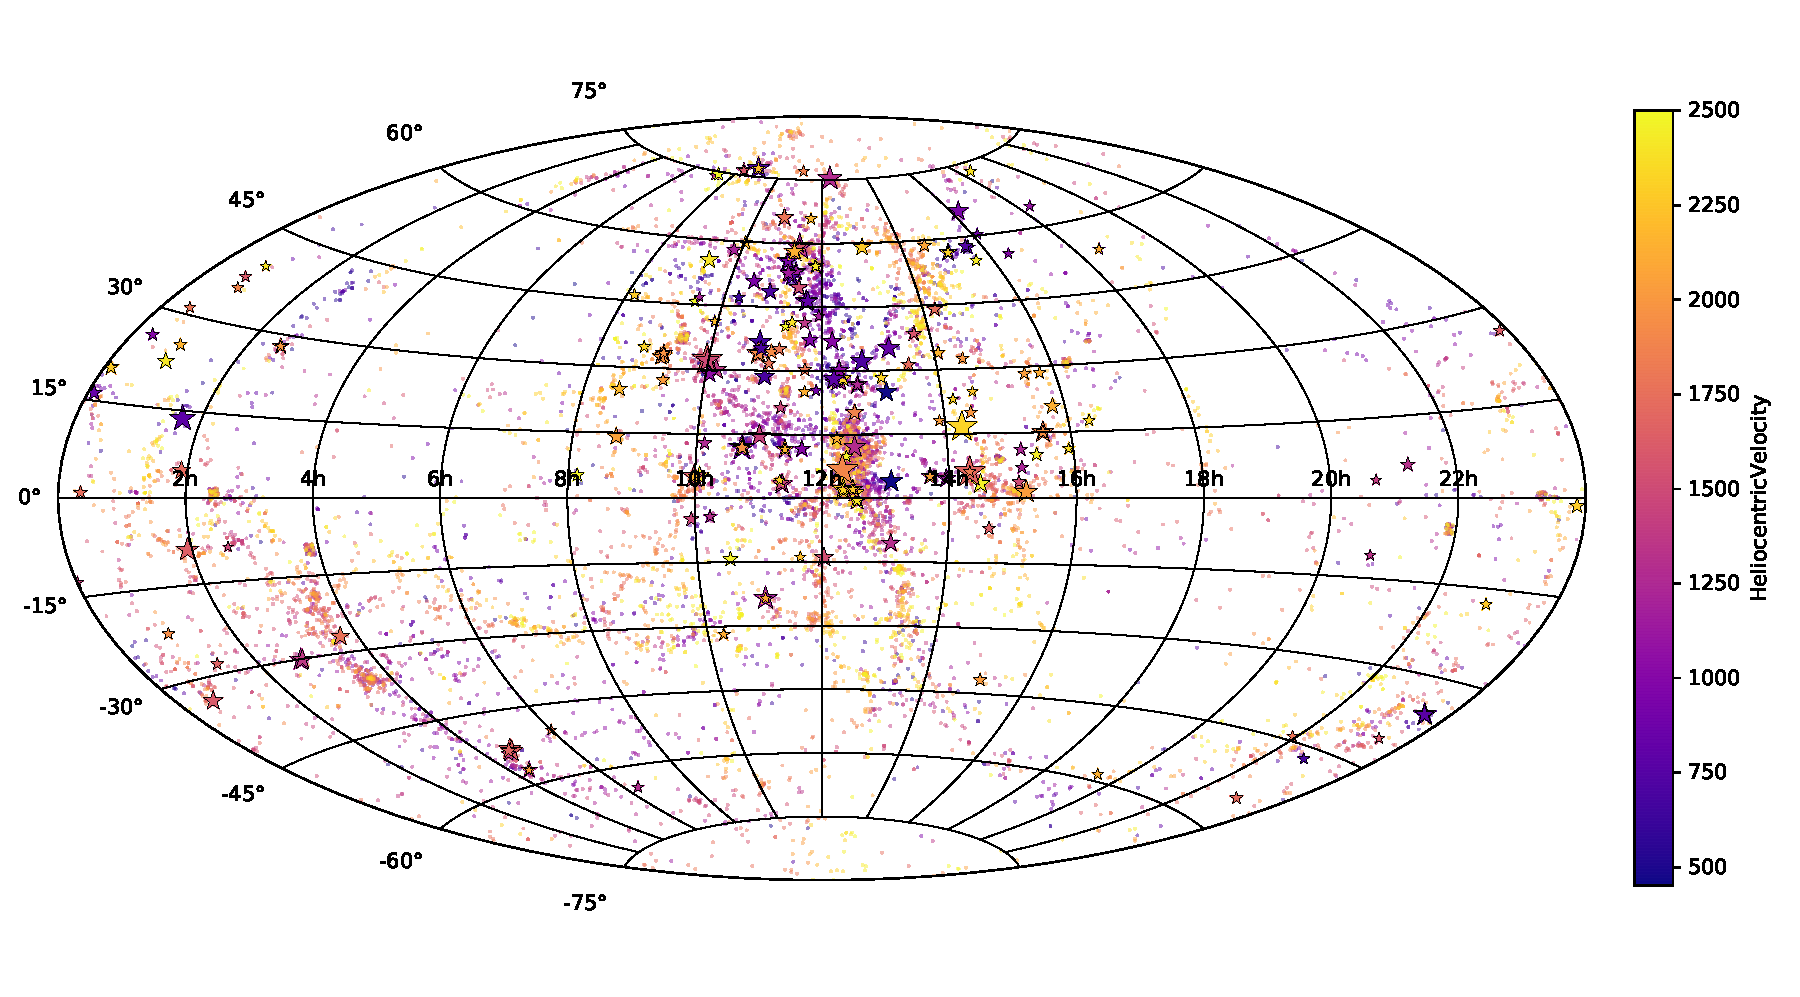
\includegraphics[width=0.94\linewidth]{Chap5/figures/2500kms_galaxies-True_12h.pdf}}\label{allsky_2500}
  \subfigure[]{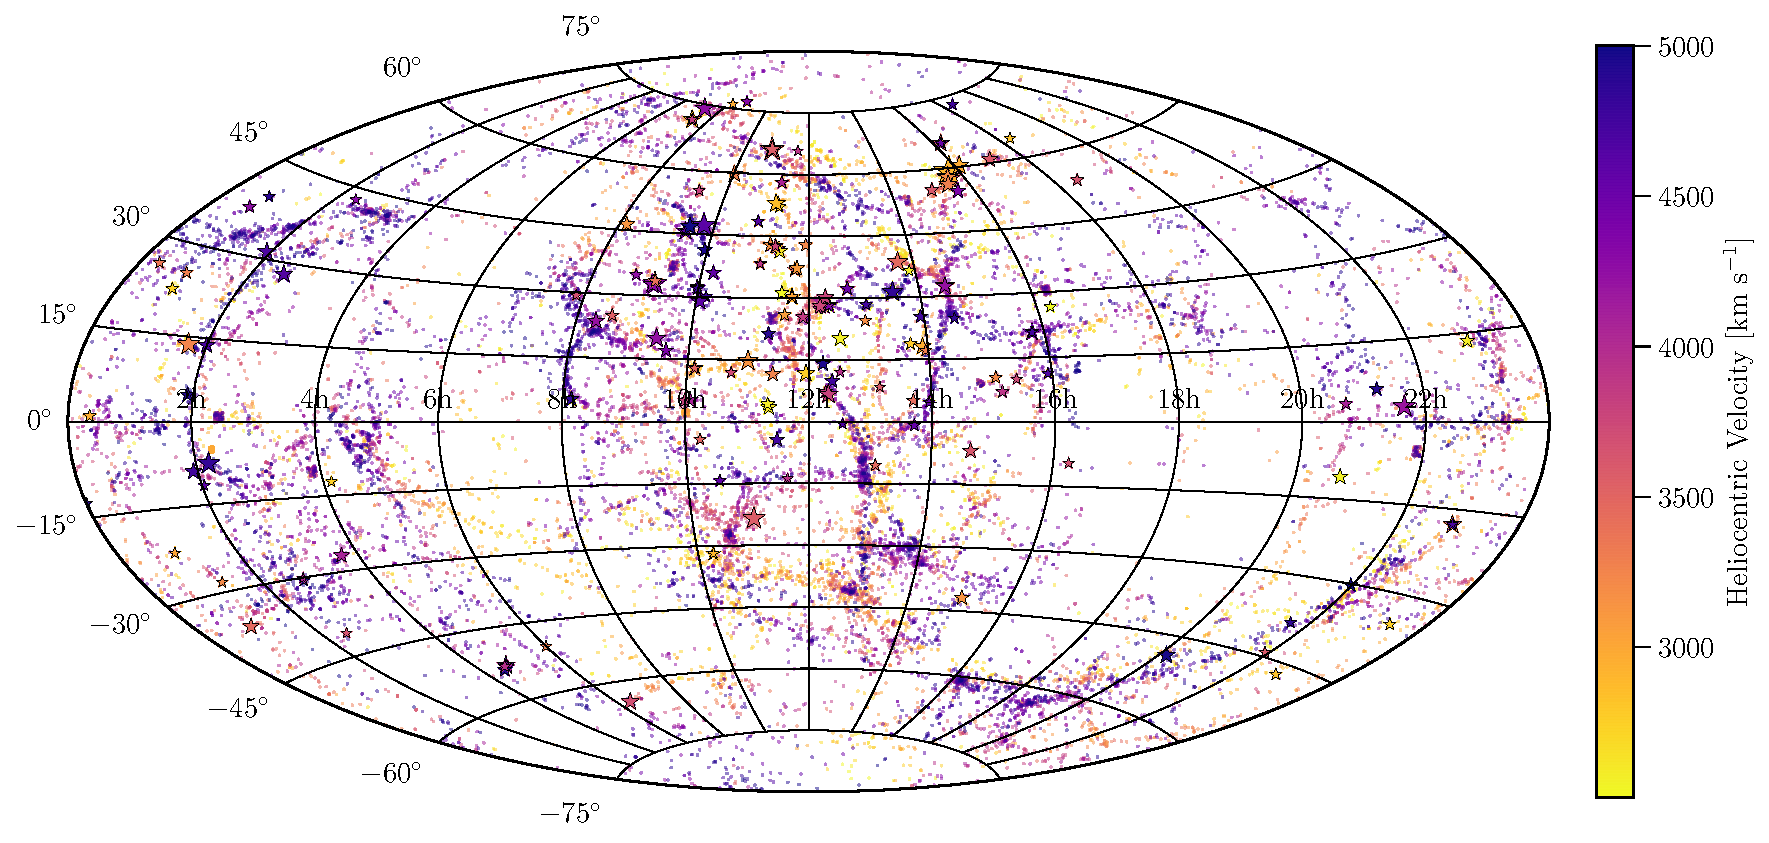
\includegraphics[width=0.94\linewidth]{Chap5/figures/5000kms_galaxies-True_12h.pdf}}\label{allsky_5000}
  \caption{\small{All sky maps of the locations of all absorbers and galaxies. Absorbers are plotted as stars and scaled in size based on their EW. Galaxies are plotted as dots. The colors of both galaxies and absorbers are mapped to their heliocentric velocities. (a) All galaxies and absorbers in the velocity range $450 \leq cz \leq 2500$ \kms. (b) All galaxies and absorbers in the velocity range $2500 < cz \leq 5000$ \kms.}}
%\vspace{-1pt}
\label{allsky_2500-5000}
\end{figure}

\begin{figure}[ht!]
%\vspace{-5pt}
\centering
  \subfigure[]{\includegraphics[width=0.94\linewidth]{Chap5/figures/7500kms_galaxies-True_12h.pdf}}\label{allsky_7500}
  \subfigure[]{\includegraphics[width=0.94\linewidth]{Chap5/figures/10000kms_galaxies-True_12h.pdf}}\label{allsky_10000}
  \caption{\small{All sky maps of the locations of all absorbers and galaxies. Absorbers are plotted as stars and scaled in size based on their EW. Galaxies are plotted as dots. The colors of both galaxies and absorbers are mapped to their heliocentric velocities. (a) All galaxies and absorbers in the velocity range $5000 < cz \leq 7500$ \kms. (b) All galaxies and absorbers in the velocity range $7500 < cz \leq 10,000$ \kms.}}
\label{allsky_7500-10000}
%\vspace{1pt}
\end{figure}

\section{Data and Analysis}

In this section we discuss the selection and reduction of our sample of archival QSO spectra taken by the Cosmic Origins Spectrograph (COS) on \textit{HST}. There currently exist over 700 COS spectra in the Barbara A. Mikulski Archive for Space Telescopes (MAST) with G130M exposures which cover the $\rm Ly\alpha$ transition in our survey's redshift range ($cz \leq 10,000$ \kms). In order to choose the most useful spectra for our purposes, we first sort them by signal-to-noise (SN) and make a cut at approximately SN=10. A signal-to-noise of approximately 10 or higher measured near $\rm 1238 \AA$ allows us to detect an absorption feature down to an equivalent width of $\rm \sim 50 m\AA$ at $5\sigma$. We then correlate the resulting (SN$\gtrsim 10$) sample with our galaxy catalog (see Chapter 2), and sort the spectra by proximity to a galaxy. While this introduces a slight bias against void or isolated absorption features, we are presently most interested in the absorber-galaxy relation and therefore choose this method to maximize the associated absorber-galaxy sample size. Additionally, because this sorting is done without knowledge of line locations, we will end up with significant sample of isolated absorbers simply based on their velocity, or $z$-direction, isolation from galaxies. Finally, from this galaxy-proximity sorted spectra list we choose 264 targets based on the relative ease of spectral feature identification. Because many of these archival sightlines were originally observed to study systems at $z > 0.03$ and not because of their proximity to any nearby galaxy, the resulting final sample is mostly randomly distributed across the sky.


%\FloatBarrier
%\begin{deluxetable}{| l | c | c | c | c |}
%%\setlength{\tabcolsep}{0.1in}
%%\tablecolumns{8}
%%\tabletypesize{\scriptsize}
%%\tablewidth{1pt}
%\tablecaption{Summary of $\mathcal{L}$ Variants \label{likelihood_variants}}
%\tablehead{
%\colhead{$\mathcal{L}$ Variant}  										&  \colhead{$\mathcal{L}-isolated$}	&  \colhead{$\mathcal{L}-associated-isolated$}	&  \colhead{$\mathcal{L}-associated$}	&  \colhead{$\mathcal{L}-two+$} 	}
%\startdata
%Total number of $\rm Ly\alpha$ absorbers: 1135 \\
%571 are $isolated$ regardless of normalization \\
%\hline
%\hline
%$\mathcal{L}_{min} = 0.01, rigor = 5$	 ($Standard$)							&	267						&	56								&	146						&	58						\\
%\hline
%$\mathcal{L}_{min} = 0.01, rigor = 5$, $A=2~if~\rho \leq R_{vir}$				&	267						&	56								&	160						&	55						\\
%\hline
%$\mathcal{L}_{min} = 0.001, rigor = 5$									&	227						&	69								&	167						&	65						\\
%\hline
%$\mathcal{L}_{min} = 0.001, rigor = 6$									&	227						&	69								&	162						&	68						\\
%\hline
%$\mathcal{L}_{min} = 0.001, rigor = 7$									&	227						&	69								&	154						&	75						\\
%\hline
%$\mathcal{L}_{min} = 0.001, rigor = 8$									&	227						&	69								&	145						&	78						\\
%\hline
%$D^{1.5}$, $\mathcal{L}_{min} = 0.001, rigor = 5$ 							&	317						&	39								&	174						&	32						\\
%\hline
%$\mathcal{L}_{min} = 0.001, rigor = 5$, $A=2~if~\rho \leq R_{vir}$				&	227						&	69								&	181						&	62						\\
%\hline
%$\mathcal{L}_{min} = 0.005$, $v_{norm} = 150, rigor = 5$						&	265						&	58								&	148						&	63						\\
%\hline
%$\mathcal{L}_{min} = 0.005$, $v_{norm} = 250, rigor = 5$						&	246						&	64								&	151						&	64						\\
%\hline
%\enddata
%\tablecomments{A summary of the subset sizes resulting from varying the likelihood metric's normalization parameters. Different choices of normalization are simply shifting some of the non-$isolated$ absorbers between different bins.}
%\end{deluxetable}
%\FloatBarrier

Data reduction, continuum fitting and line measurement are then conducted in an identical fashion to \cite{french2017}. In short, we determine the continuum around each line by fitting a 1st, 2nd or 3rd order polynomial to the line-free regions around each feature. All equivalent width measurements are integrated based on this fit, and we calculate the second moment of the apparent optical depth profiles to determine Doppler $b$-parameters. Table \ref{QSOsample}, located in the Appendix, summarizes the QSO targets included in this work.

In this sample of 264 QSOs we have detected 1135 Ly$\alpha$ absorbers. Figures \ref{allsky_2500-5000} and \ref{allsky_7500-10000} show all-sky maps of the positions of all absorbers split into 4 velocity bins ($v_{\rm Ly\alpha} = [0 - 2500]$, $(2500 - 5000]$, $(5000 - 7500]$, and $(7500 - 10,000]$ \kms). The distribution of galaxies in the same velocity ranges are include here also (galaxies are plotted as small circles, absorbers as stars; see Chapter 2). Comparing the galaxy to absorber positions and velocities within each velocity range by eye, we can clearly see that the Ly$\alpha$ absorbers broadly trace the locations of the galaxies. If the current Lambda Cold Dark Matter ($\Lambda$CDM) cosmology is to be believed, this should not be remarkably surprising. The baryons from which galaxies are built and those found within the IGM and traced by $\rm Ly\alpha$ absorption should both follow the underlying potential produced by the Dark Matter, and should therefore be found in similar places. Beyond this big-picture result however, we want to know how the absorbers react to the presence of the galaxies on a more local scale.

% this table is from pickle version 8 results

\subsection{Sub-sample selection}

A major hurdle for galaxy-absorber correlation studies has always been matching any particular absorption line to a single nearby galaxy. The basic premise of matching relies on the assumption that, in at least some cases, one particular galaxy's potential, angular momentum, and radiation field dominates what an absorber ``feels" (i.e., is the primary influencer for the EW, column density and Doppler $b$-parameter of an absorber). With this assumption in place, the issue becomes that galaxies are generally not isolated. When faced with a distribution of galaxies of differing types, sizes, orientations and distances (impact parameters) and velocities ($\Delta v = v_{\rm absorber} - v_{\rm galaxy}$) from an absorption line, which, if any, are most likely to be ``associated" with the line? 

As first introduced in \cite{french2017}, we employ a unique likelihood method for objectively matching absorbers with nearby galaxies in a consistent, analytical manner. We define likelihood, $\mathcal{L}$, as follows: 

\begin{equation}
\mathcal{L} = A \times e^{-(\frac{\rho}{R_{\rm eff}})^2} \times e^{-(\frac{\Delta v}{v_{\rm norm}})^2},
\label{likelihood}
\end{equation}

\noindent where $A$ is a normalization constant, $\rho$ is the impact parameter between a galaxy and sightline, $R_{\rm eff}$ is one of two possible ``effective - radii" we use for galaxies (virial radius and $D^{1.5}$, or diameter to the 1.5 power), $\Delta v$ is the velocity separation between absorber and galaxy heliocentric, and $v_{\rm norm}$ is a velocity normalization (equal to one of 150, 200, or 250). 

We calculate $\mathcal{L}$ for every absorber-galaxy combination, which then gives us a single number as a three-dimensional proxy for the physical separation between the two. Based on this $\mathcal{L}$ we then separate our sample into the following 5 distinct bins: $isolated$, $\mathcal{L}-isolated$, $\mathcal{L}-associated-isolated$, $\mathcal{L}-associated$, and $\mathcal{L}-two+$. The $isolated$ sample contains all the $\rm Ly\alpha$ lines that are farther than 500 kpc and 400 \kms~from \emph{any} galaxy. The $\mathcal{L}-isolated$ sample contains those $\rm Ly\alpha$ lines are far enough away from any galaxy so as to not meet our minimum-$\mathcal{L}$ criteria. The $\mathcal{L}-associated-isolated$ sample contains those $\rm Ly\alpha$ lines which meet our $\mathcal{L}$ criteria to be associated with a single galaxy, and that galaxy is isolated by 500 kpc and 400 \kms. The $\mathcal{L}-associated$ sample contains those $\rm Ly\alpha$ lines which meet our $\mathcal{L}$ criteria to be associated with a single galaxy, but that galaxy is \emph{not} isolated. And finally, the $\mathcal{L}-two+$ sample contains those  $\rm Ly\alpha$ lines which meet our minimum-$\mathcal{L}$ criteria to be associated with \emph{more} than one galaxy.

\begin{deluxetable}{| l | c | c | c | c |}
\tabletypesize{\footnotesize}
\rotate
\tablewidth{0pt}
\tablecaption{Summary of $\mathcal{L}$-Variants \label{likelihood_variants}}
\tablehead{
\colhead{$\mathcal{L}$ Variant}  										&  \colhead{$\mathcal{L}-isolated$}	&  \colhead{$\mathcal{L}-associated-isolated$}	&  \colhead{$\mathcal{L}-associated$}	&  \colhead{$\mathcal{L}-two+$} 	}
\startdata
Total number of $\rm Ly\alpha$ absorbers: 1135 \\
571 are $isolated$ regardless of normalization \\
\hline
\hline
$\mathcal{L}_{min} = 0.01, rigor = 5$	 ($Standard$)							&	267						&	56								&	146						&	58						\\
\hline
$\mathcal{L}_{min} = 0.01, rigor = 5$, $A=2~if~\rho \leq R_{vir}$				&	267						&	56								&	160						&	55						\\
\hline
$\mathcal{L}_{min} = 0.001, rigor = 5$									&	227						&	69								&	167						&	65						\\
\hline
$\mathcal{L}_{min} = 0.001, rigor = 6$									&	227						&	69								&	162						&	68						\\
\hline
$\mathcal{L}_{min} = 0.001, rigor = 7$									&	227						&	69								&	154						&	75						\\
\hline
$\mathcal{L}_{min} = 0.001, rigor = 8$									&	227						&	69								&	145						&	78						\\
\hline
$D^{1.5}$, $\mathcal{L}_{min} = 0.001, rigor = 5$ 							&	317						&	39								&	174						&	32						\\
\hline
$\mathcal{L}_{min} = 0.001, rigor = 5$, $A=2~if~\rho \leq R_{vir}$				&	227						&	69								&	181						&	62						\\
\hline
$\mathcal{L}_{min} = 0.005$, $v_{norm} = 150, rigor = 5$						&	265						&	58								&	148						&	63						\\
\hline
$\mathcal{L}_{min} = 0.005$, $v_{norm} = 250, rigor = 5$						&	246						&	64								&	151						&	64						\\
\hline
\enddata
\tablecomments{A summary of the subset sizes resulting from varying the likelihood metric's normalization parameters. Different choices of normalization are simply shifting some of the non-$isolated$ absorbers between different bins.}
\end{deluxetable}


Our standard criteria for a positive galaxy-absorber association are $\mathcal{L} \geq 0.01$ and $\mathcal{L}_1 \geq rigor \times \mathcal{L}_2$ with $rigor =5$ (i.e., the $\mathcal{L}$-value for the most likely associated galaxy must be at least 5 times greater than that for the second most likely galaxy). However, we have also explored the results of adjusting the several possible $\mathcal{L}$ normalizations. We calculate $\mathcal{L}$ with $R_{\rm eff}$ equal to $R_{\rm vir}$ and $D^{1.5}$ and $v_{\rm norm}$ equal to 150, 200, and 250. For each of these combinations, we also calculate a variant with $A =1$ and another with $A = 2$ if $R_{\rm eff} \ge \rho$, and $A=1$ otherwise. Additionally, we investigate the effect of changing the minimum-$\mathcal{L}$ criteria to 0.005 and 0.001, and $rigor$ = 5, 6, 7, and 8. Table \ref{likelihood_variants} summarizes the resulting subsets for each of these combinations. 


Overall, we find that none of these adjustments have a major effect on the resulting samples. To check, we performed Anderson-Darling statistical distribution analyses to check for differences between the EW distributions for each $\mathcal{L}$-variant and found no statistically significant difference between matching subsets (e.g., the EW distribution for the $\mathcal{L}-associated$ subset does not change significantly between these different $\mathcal{L}$ variants). For the remainder of this analysis we will concentrate on the $\mathcal{L}_{\rm min} = 0.01, v_{\rm norm} = 200$, $A = 2$ normalization subsets. This matches the normalization we adopted in \cite{french2017}, and represents a middle ground option while also maximizing the size of the $\mathcal{L}-isolated-associated$, $\mathcal{L}-associated$, and $\mathcal{L}-two+$ subsets.




%For the remainder of this analysis we will concentrate on the $\mathcal{L}_{\rm min} = 0.005, v_{\rm norm} = 250$ normalization subsets. This represents a middle ground option while also maximizing the size of the $\mathcal{L}-isolated-associated$, $\mathcal{L}-associated$, and $\mathcal{L}-two+$ subsets. \textbf{MORE}


%($A=1$, $R_{eff} = R_{vir}$, $v_{norm} = 200$, $\mathcal{L}_{min} = 0.01$)


\section{Results \& Discussion}
\subsection{Detection Fraction}
First we explore the $\rm Ly\alpha$ detection fraction as a function of galaxy proximity. To calculate this, we start by correlating the position of every QSO with our galaxy sample. For every galaxy found within 1000 kpc in physical impact parameter of each sightline we then check if a $\rm Ly\alpha$ line appears in that sightline and within 400 \kms~of the galaxy's systemic velocity. This results in a detection fraction as a function of impact parameter. Additionally, we calculate the detection fraction as a function of likelihood, $\mathcal{L}$, in a similar manner. However, as we are calculating detection fraction without any a priori knowledge of the velocity of the absorption lines, the likelihood function we use is modified from Eq. \ref{likelihood} to simply $e^{-(\rho/R_{vir})^2}$, or only the impact parameter - virial radius portion of our usual likelihood function given by Eq. \ref{likelihood}. Note that this adjusted likelihood function is identical to Eq. \ref{likelihood} when $\Delta v = 0$. 

\begin{figure}[t!]
        \centering
        \vspace{0pt}
%        \includegraphics[width=0.49\textwidth]{detection_fraction_both_err.pdf}
        \includegraphics[width=0.99\textwidth]{Chap5/figures/detection_fraction_min0_50_100_200_300_both_alt4.pdf}
        \caption{\small{The detection fraction as a function of impact parameter (grey-circles) and $\mathcal{L}$ (blue-diamonds). Note that the impact parameter and $\mathcal{L}$ $x$-axis scales are quite different; the lowest $\mathcal{L}$ bin (0.0001) corresponds to $\sim 3 R_{\rm vir}$, whereas the largest impact parameter bin (1000 kpc) is generally $\gg 3 R_{\rm vir}$. Error bars show the $1\sigma$ Poisson errors.}}
        \vspace{0pt}
        \label{detection_fraction}
\end{figure}


%\begin{figure}[ht!]
%        \centering
%        \vspace{15pt}
%        \subfigure[]{\includegraphics[width=0.49\textwidth]{Chap5/figures/hist(EW)_bins10_6_EWcut50-15000_err_dataset_double.pdf}\label{cdf_ew}}
%       
%        \subfigure[]{\includegraphics[width=0.49\textwidth]{Chap5/figures/hist(b)_all6_bins1_EWcut50-10000_errTrue_dataset_double.pdf}\label{cdf_b}}
%        \caption{\small{The equivalent width (a) and Doppler $b$-parameter (b) cumulative distribution functions for each subset of our Ly$\alpha$ absorber sample. From the top-left corner to the bottom-right the curves are the fully isolated absorbers (grey), the absorbers isolated enough from any galaxy to not be likelihood-matched (brown), the full distribution (black), the absorbers likelihood-matched to a single, non-isolated galaxy (orange), the absorbers matched to a single, isolated galaxy (green), and the absorbers likelihood-matched with two or more galaxies (purple). The shaded region around each curve gives the EW ($b$-parameter) measurement errors. Only $\rm EW \ge 50~m\AA$ absorbers are included to mitigate any bias due to the detection limit of lower-SN targets.}}
%        \vspace{5pt}
%        \label{ew_both}
%\end{figure}




\begin{figure}[ht!]
        \centering
        \subfigure[]{\includegraphics[width=0.99\textwidth]{Chap5/figures/hist(EW)_bins10_6_EWcut50-15000_err_dataset_double.pdf}\label{cdf_ew}}
        \caption{\small{The equivalent width cumulative distribution functions for each subset of our Ly$\alpha$ absorber sample. From the top-left corner to the bottom-right the curves are the fully isolated absorbers (grey), the absorbers isolated enough from any galaxy to not be likelihood-matched (brown), the full distribution (black), the absorbers likelihood-matched to a single, non-isolated galaxy (orange), the absorbers matched to a single, isolated galaxy (green), and the absorbers likelihood-matched with two or more galaxies (purple). The shaded region around each curve gives the EW measurement errors. Only $\rm EW \ge 50~m\AA$ absorbers are included to mitigate any bias due to the detection limit of lower-SN targets.}}
        \label{ew_both}
\end{figure}


\begin{figure}[ht!]
        \centering
        \subfigure[]{\includegraphics[width=0.99\textwidth]{Chap5/figures/hist(b)_all6_bins1_EWcut50-10000_errTrue_dataset_double.pdf}\label{cdf_b}}
        \caption{\small{The Doppler $b$-parameter cumulative distribution functions for each subset of our Ly$\alpha$ absorber sample. From the top-left corner to the bottom-right the curves are the fully isolated absorbers (grey), the absorbers isolated enough from any galaxy to not be likelihood-matched (brown), the full distribution (black), the absorbers likelihood-matched to a single, non-isolated galaxy (orange), the absorbers matched to a single, isolated galaxy (green), and the absorbers likelihood-matched with two or more galaxies (purple). The shaded region around each curve gives the $b$-parameter measurement errors. Only $\rm EW \ge 50~m\AA$ absorbers are included to mitigate any bias due to the detection limit of lower-SN targets.}}
        \label{ew_both}
\end{figure}




%\begin{figure}[ht!]
%        \centering
%        \vspace{15pt}
%        \includegraphics[width=0.48\textwidth]{hist(EW)_bins10_6_EWcut50-15000_err_dataset_double.pdf}
%        \caption{\small{The equivalent width (EW) cumulative distribution function for each subset of our Ly$\alpha$ absorber sample. From the top-left corner to the bottom-right the curves are the fully isolated absorbers (grey), the absorbers isolated enough from any galaxy to not be likelihood-matched (brown), the full distribution (black), the absorbers likelihood-matched to a single, non-isolated galaxy (orange), the absorbers matched to a single, isolated galaxy (green), and the absorbers likelihood-matched with two or more galaxies (purple). The shaded region around each curve gives the EW measurement errors. Only $\rm EW \ge 50~m\AA$ absorbers are included to mitigate any bias due to the detection limit of lower-SN targets.}}
%        \vspace{0pt}
%        \label{cdf_ew}
%\end{figure}
%
%\begin{figure}[t!]
%        \centering
%        \vspace{0pt}
%%        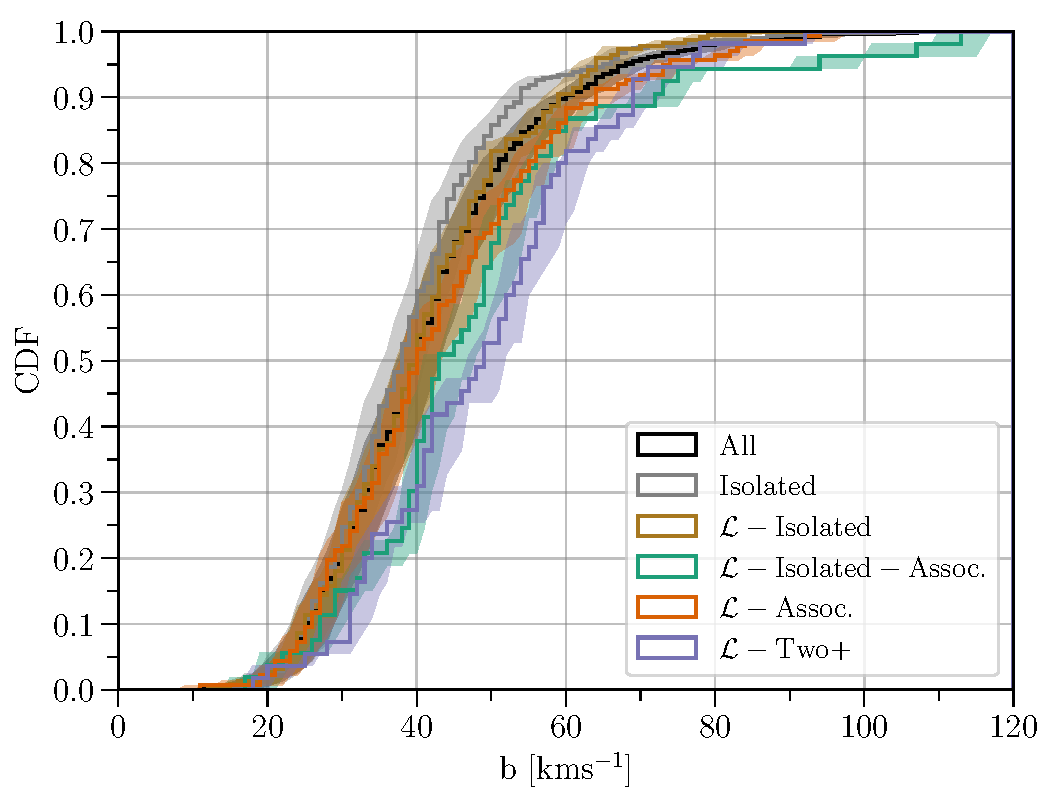
\includegraphics[width=0.49\textwidth]{hist(b)_all6_bins1_EWcut50-10000_errTrue_dataset.pdf}
%        \includegraphics[width=0.49\textwidth]{hist(b)_all6_bins1_EWcut50-10000_errTrue_dataset_double.pdf}
%        \caption{\small{The Doppler $b$-parameter ($b$) cumulative distribution function for each subset of our Ly$\alpha$ absorber sample. From the top-left corner to the bottom-right the curves are the fully isolated absorbers (grey), the absorbers isolated enough from any galaxy to not be likelihood-matched (brown), the full distribution (black), the absorbers likelihood-matched to a single, non-isolated galaxy (orange), the absorbers matched to a single, isolated galaxy (green), and the absorbers likelihood-matched with two or more galaxies (purple). The shaded region around each curve gives the $b$-parameter measurement errors. Only $\rm EW \ge 50~m\AA$ absorbers are included to mitigate any bias due to the detection limit of lower-SN targets.}}
%        \vspace{5pt}
%        \label{cdf_b}
%\end{figure}

We have plotted the detection fraction as a function of both impact parameter and $\mathcal{L}$ in Figure \ref{detection_fraction}. We also display the detection fraction for minimum $\rm Ly\alpha$ EWs of 50, 100, 200, and 300 $\rm m\AA$ in purple, green, yellow, and red (respectively). As expected, the detection fraction clearly increases with decreasing impact parameter and increasing $\mathcal{L}$. Additionally, the detection fraction curves for higher EW absorbers increasingly become steeper. Hence, the detection fraction for strong absorbers is very low at large impact parameter or $\mathcal{L}$, but climbs quickly back to $\gtrsim 70\%$ within $\sim 100$ kpc or $0.1 \mathcal{L}$. 

We also note that while the detection fraction as a function of impact parameter continues to rise all the way to the 25 kpc mark, it levels off at $\sim 1.5 R_{\rm vir}$ ($\sim 0.1 \mathcal{L}$) as a function of likelihood. Perhaps this represents the edge of the CGM; beyond $\sim 1.5 R_{\rm vir}$ we are increasingly detecting the large-scale filaments that the galaxies reside in, and inside this radius we reach a nearly constant $\sim85\%$ covering fraction. The fact that the detection fraction remains at $\gtrsim 50\%$ all the way to (and possibly past) 1 Mpc further suggests this important contribution of general Cosmic Web absorbers to the aggregate sample.


\subsection{Equivalent Width}
Here we explore the effect of environment on the equivalent width of our $\rm Ly\alpha$ absorber sample. Figure \ref{cdf_ew} shows the cumulative distribution function of equivalent widths for each of our 5 likelihood-separated subsets, along with that of the entire sample in black). We have only included $\rm EW \ge 50~m\AA$ here to mitigate any bias due to the detection limit of lower-SN targets. We find that each subset occupies a distinct space aside from the $\mathcal{L}-associated-isolated$ and $\mathcal{L}-associated$ sets, which are essentially indistinguishable. The physical result of this is that the strength EW of $\rm Ly\alpha$ absorption depends strongly on environment. Stronger absorption lines are preferentially found near to galaxies, and the strongest lines are found near multiple galaxy systems. The result of Anderson-Darling statistical distribution tests between each subset indicate that our $isolated$ and $\mathcal{L}-isolated$ subsets are distinct from each of $\mathcal{L}-two+$, and $\mathcal{L}-associated-isolated$ and $\mathcal{L}-associated$ at a $\gg 5 \sigma$ level. Because $\mathcal{L}-associated-isolated$ and $\mathcal{L}-associated$ are found to be nearly indistinguishable via these test and by-eye, we will combine them for the remainder of this analysis.


This separation between EW distributions based on galaxy proximity is likely an effect of the distribution of the cosmic web; multiple galaxies should form from denser sections and intersections of intergalactic filaments, and these environments should thus also produce a stronger absorption profile. Indeed, many previous studies have found similar results, with weak $\rm Ly\alpha$ correlating only weakly with the positions of galaxies compared to either the strong absorber-galaxy or galaxy-galaxy correlations (see e.g., \citealt{chen2005, morris2006, wilman2007, chen2009}). Here we find that nearly $\rm 95\%$ of EW $\rm \leq 400~m\AA$ are found farther than 500 kpc and $\rm 400$ \kms~ from any $L \gtrsim 0.1$\Lstar~galaxy. These weak $\rm Ly\alpha$ lines are thus likely tracing the underlying larges-scale filamentary structures, and \emph{not} individual galaxy halos (see \citealt{tripp1998, wakker2015} also).


\begin{figure}[ht!]
        \centering
        \vspace{0pt}
        \subfigure[]{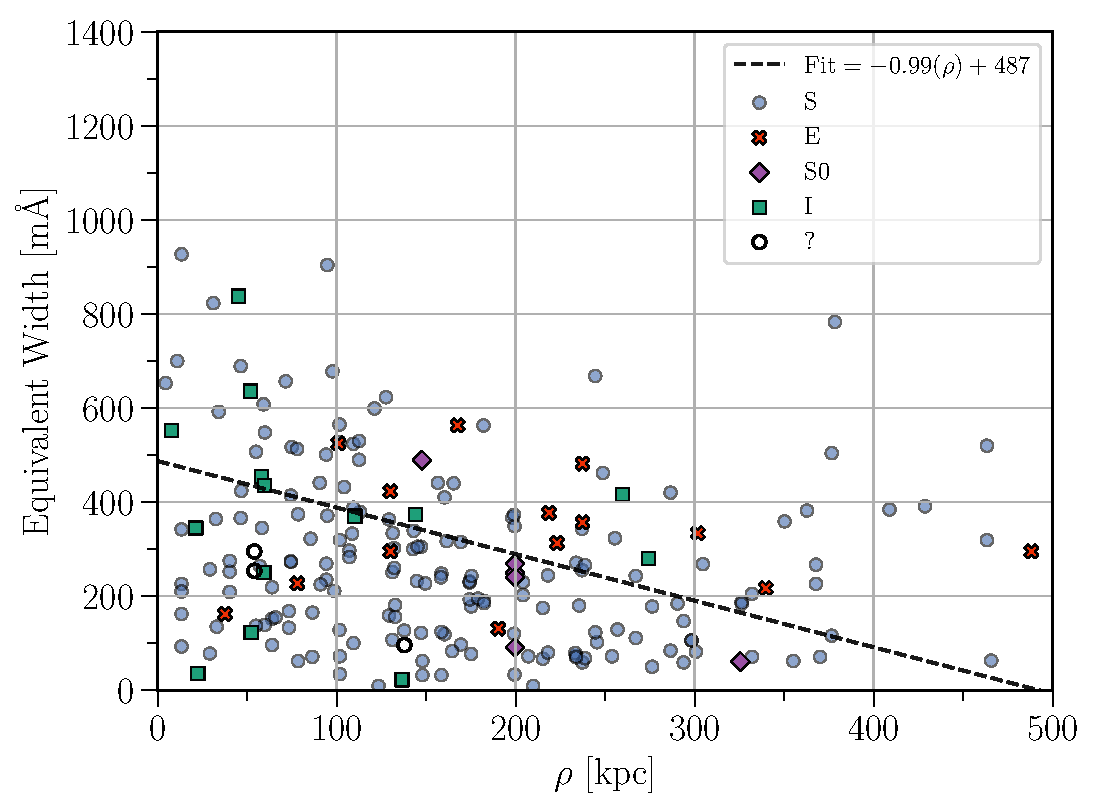
\includegraphics[width=0.49\textwidth]{Chap5/figures/W(impact)_MType_binSize50_EWcut0-10000_dataset_double.pdf}\label{ew_impact}}
        \subfigure[]{\includegraphics[width=0.49\textwidth]{Chap5/figures/W(impact_vir)_MType_binSize0_5_EWcut0-10000_dataset_double.pdf}\label{ew_impact_rvir}}
        \caption{\small{\textbf{Left: } The equivalent width (EW) of absorbers a function of impact parameter ($\rho$) to the associated galaxy. The best fit shown by the dashed-black line has the form: $EW = m (\rho) + b,$ with $m = -0.99 \pm 0.25$ and $b = 487 \pm 49$. \textbf{Right:} The EW of absorbers a function of impact parameter to the associated galaxy normalized by the galaxy virial radius ($\rho / R_{\rm vir}$). The best fit shown by the dashed-black line has the form: $EW = m (\rho / R_{\rm vir}) + b,$ with $m = -265 \pm 48$ and $b = 620 \pm 59$. \textbf{Both:} All $\mathcal{L}-associated-isolated$ and $\mathcal{L}-associated$ systems are included here. Blue-circles indicate spiral-type galaxies, green-squares indicate irregulars, red-crosses indicate ellipticals, purple-diamonds indicate S0's, and open black-circles indicate ambiguous morphological types. }}
        \vspace{5pt}
        \label{ew_both}
\end{figure}


This result on it's own does not however illuminate any deeper connection or relationship between the individual galaxies and absorbers. Let us now consider the dependence of EW on galaxy impact parameter, as illustrated in Figure \ref{ew_impact}. We have also plotted EW as a function of virial radius normalized impact parameter ($\rho/ R_{\rm vir}$) in Figure \ref{ew_impact_rvir}. Firstly, we notice that weak ($\rm EW \lesssim 400~m\AA$) absorbers are found at all impact parameters and $\rho / R_{\rm vir}$, which agrees with our findings above from Figure \ref{cdf_ew}. Moreover, absorbers stronger than $\rm EW \sim 400~m\AA$ are preferentially found close to galaxies, and absorbers with $\rm EW \sim 800~m\AA$ are \emph{only} found within 100 kpc and $1 R_{\rm vir}$. Hence, weak $\rm EW \lesssim 400~m\AA$ absorbers are most likely $\rm Ly\alpha$-forest material, while the stronger absorbers are associated with the galaxies.

Secondly, we have included linear fits in both Figures \ref{ew_impact} and \ref{ew_impact_rvir} as shown by the dashed-black lines. In each case we find a strong negative slope, and by eye the virial radius normalized version appearing to be the stronger correlation. To test this we calculated the Pearson correlation coefficient $r$-value for each fit. For the purely impact parameter correlation we find a Pearson $r$-value $=-0.26$, with a $p$-value of $p = 1.2 \times 10^{-4}$, which indicates a weak but statistically significant negative correlation. For the virial radius normalized correlation we find $r = -0.35$ with $p = 1.2 \times 10^{-7}$, indicating a stronger and \emph{more significant} negative correlation. If true, then the EW of $\rm Ly\alpha$ absorption depends on the size of galaxy halos. Hence, either the physical or number density (or both) of absorbing cloudlets is greater closer to galaxies in a halo-scale dependent manner. The increased density of this neutral material could signify both inflows or outflows from galaxies, with inflows expected to harbor a greater fraction of the cool, neutral \HI~most readily traced by $\rm Ly\alpha$. An analysis of metals associated with these neutral cloudlets could provide clues to which is the mechanism source at play here.

Thirdly, let us consider the effect of galaxy morphology on the associated absorption, which we have indicated in Figure \ref{ew_both} by the color and style of the plot points. In each figure blue-circles indicate spiral-type galaxies, green-squares indicate irregulars, red-crosses indicate ellipticals, purple-diamonds indicate S0's, and open black-circles indicate ambiguous or unknown types. Spiral galaxies are clearly the dominant type, and are found at all impact parameter and EW. Irregulars are the next most common, but are not spread around as evenly. All but two irregular-type systems are separated by less than 150 kpc in Figure \ref{ew_impact}, and few low-EW absorbers are found within $\sim 0.5 R_{\rm vir}$ in Figure \ref{ew_impact_rvir}. In the first case, this can be explained by irregulars having a smaller average size ($\overline{R}_{\rm vir} = 101$ kpc for irregulars, compared to 145, 178, and 194 kpc for spirals, S0's, and ellipticals). When normalized by virial radius however, the lack of low-EW absorbers at low $\rho / R_{\rm vir}$ could be an indication of more gas-rich halos. This would make sense, since irregular galaxies are often tidally disturbed due to recent interactions which can result in extended, gas-rich halos.

Finally, we also see that elliptical and S0 galaxies are associated with mostly low-EW absorption, especially within 100 kpc and $\sim 0.5 R_{\rm vir}$. It has been suggested that ionized metal material (e.g., O\VI~\citealt{tumlinson2011} and references therein) is deficient around early-type galaxies, and also that the absorber-galaxy clustering is weaker for these systems compared to late-type galaxies \cite{chen2005}. Our results here are consistent with this picture, and physically may be explained by a combination of a lack of star formation driven winds, shock-heating, and an overall dearth of cool gas within early type galaxy halos.


\subsection{Doppler $b$-parameter}

Here we explore the effect of environment on the Doppler $b$-parameter of our $\rm Ly\alpha$ absorber sample. In an analogous fashion as above, Figure \ref{cdf_b} shows the cumulative distribution functions for the Doppler $b$-parameters of each subset of absorbers. Similar to the EW result, the Doppler $b$-parameters trend toward larger values based on their proximity to galaxies. The separation here however is far weaker. While the separation between, e.g., $isolated$ and $\mathcal{L}-two+$ samples, remains statistically significant, we cannot claim any further significance between the other subsets. 

\begin{figure}[ht!]
        \centering
        \vspace{0pt}
        \subfigure[]{\includegraphics[width=0.47\textwidth]{Chap5/figures/b(impact)_MType_binSize50_EWcut0-10000_dataset_double.pdf}\label{b_impact}}
        \subfigure[]{\includegraphics[width=0.47\textwidth]{Chap5/figures/b(impact)_MType_binSize50_EWcut0-400_dataset_double.pdf}\label{b_impact_maxEW}}
        \subfigure[]{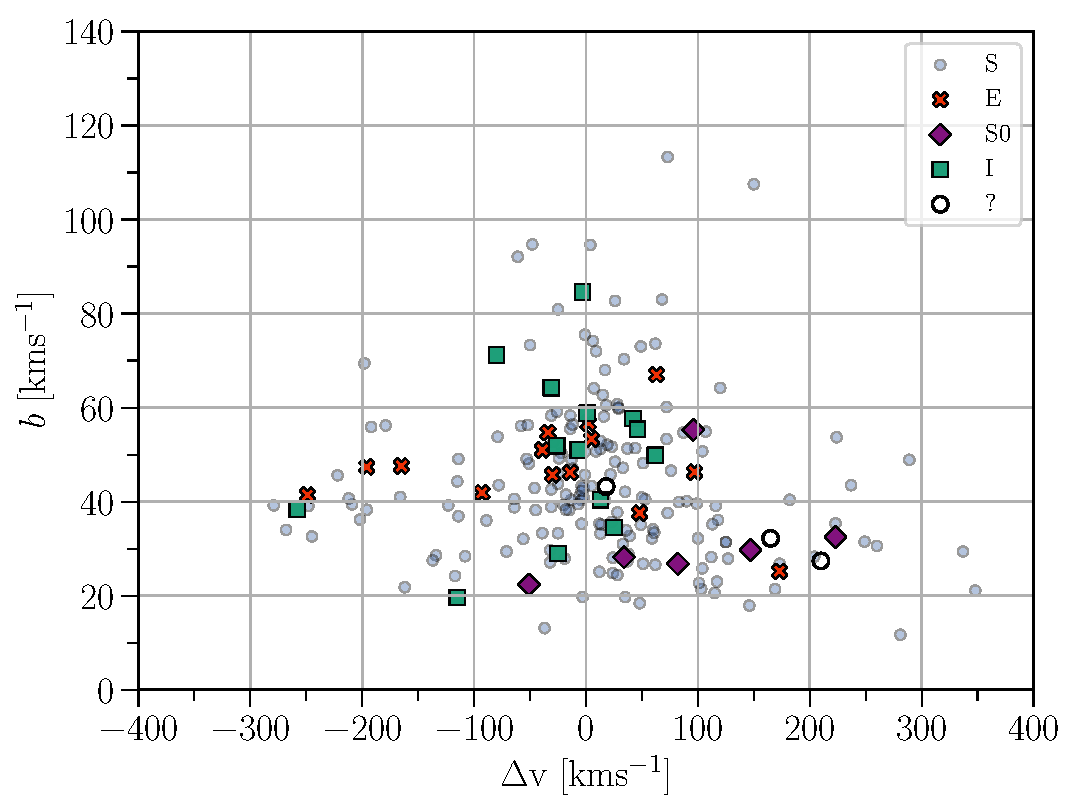
\includegraphics[width=0.47\textwidth]{Chap5/figures/b(dv)_MType_binSize50_EWcut0-10000_dataset_double.pdf}\label{b_dv}}
        \subfigure[]{\includegraphics[width=0.47\textwidth]{Chap5/figures/b(dv)_MType_binSize50_EWcut0-400_dataset_double.pdf}\label{b_dv_maxEW}}
        \caption{\small{(a) The median inclination of galaxies is shown as a function of likelihood $\mathcal{L}$ for both detection (blue-diamonds) and non-detections (red-crosses) of associated absorbers. Detection and non-detection median inclinations are also shown for minimum EW $\rm \ge 200~ m\AA$ absorber equivalent widths by the thinner, semi-transparent lines. (b) The detection fraction plotted directly as a function of inclination for systems inside (blue-diamonds) and outside (red-crosses) $1.5 \rho / R_{\rm vir}$.}}
        \vspace{5pt}
        \label{b_all}
\end{figure}




\begin{figure}[]
\centering
  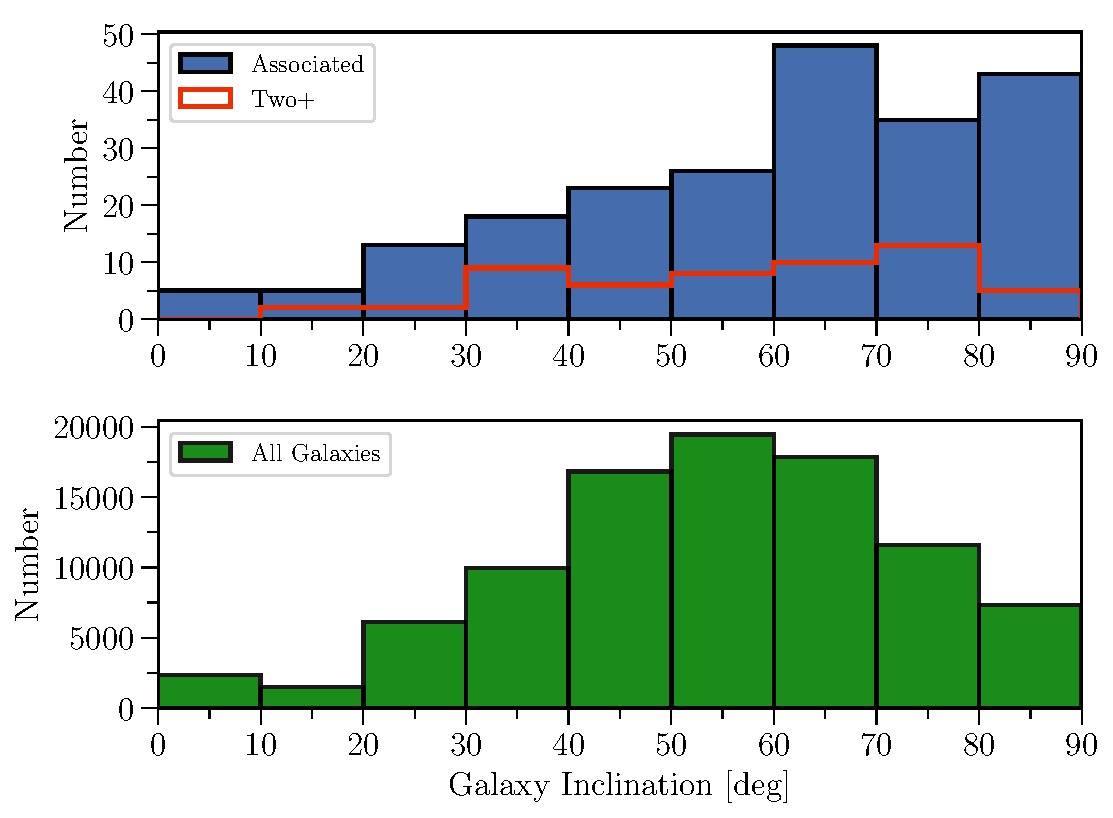
\includegraphics[width=0.9\linewidth]{Chap5/figures/hist(adjustedInc)_associated_group_all_overlaid_double.pdf}
  \caption{\small{\textbf{Top:} The distribution of all associated galaxy inclinations is shown in blue. The overlaid red histogram shows the distribution of the highest $\mathcal{L}$-galaxy inclinations from the $\mathcal{L}-two+$ subset. \textbf{Bottom:} The distribution of all galaxies in the survey volume (i.e., $cz \leq 10,000$ \kms).}}
\label{inc_hist}
\vspace{0pt}
\end{figure}

Our $b$-parameters are derived via the second moment of the apparent optical depth profile, and therefore these $b$-parameter estimates become highly uncertain for EW $\rm \gtrsim 350~m\AA$. For these stronger lines the profile becomes saturated, producing a degeneracy between EW and $b$. Unfortunately these are the very lines we expect to be most associated with near or multiple galaxy galaxy systems. This issue is illustrated by Figure \ref{b_all}, where we have show the $b$-parameters as a function of impact parameter and $\Delta v$  for the full sample (Figures \ref{b_impact} and \ref{b_dv}) and for only those systems with EW $\rm \leq 400 m\AA$ (Figures \ref{b_impact_maxEW} and \ref{b_dv_maxEW}). While a strong correlation is implied between $b$ and $\rho$ without any cuts, this completely disappears once the stronger absorbers are removed. A similar albeit less extreme effect is seen for $b$ as a function of $\Delta v$. A careful profile fitting analysis is the best way forward here, which we will reserve for a future work.


\subsection{Inclination}

Here we investigate the inclination dependence of $\rm Ly\alpha$ absorber properties. In Figure \ref{inc_hist} we display the distribution of all associated galaxies alongside the distribution of all galaxy inclinations in the survey volume (again, $\mathcal{L}-associated-isolated$ and $\mathcal{L}-associated$ subsets are combined here; see Chapter 2 for a full discussion of our galaxy dataset). As we first discovered in \cite{french2017}, there is an overabundance of absorbers associated with high-inclination galaxies. To test the significance of this overabundance we used the Anderson-Darling statistical distribution test, which yields a $p$-value of $AD_p = 7.2 \times 10^{-6}$. For a normal distribution this corresponds to $\sim 4.5 \sigma$, indicating with a high confidence limit that these associated galaxies are \emph{not} drawn from the same distribution as the all-sky galaxy population.


To further explore this phenomenon we have also calculated the detection fraction as a function of inclination and likelihood $\mathcal{L}$. Figure \ref{detection_fraction_inc} shows the median inclination as a function of $\mathcal{L}$ for galaxies. For a galaxy at a given value of $\mathcal{L}$, the solid blue-diamond line gives the median inclination if we detect an absorber within $\Delta v \leq 400$ \kms, and the dashed blue-cross line gives the same for systems \emph{without} a $\rm Ly\alpha$ detection. The error bars shown are calculated by a 10,000 repetition bootstrap analysis with replacement (i.e., we randomly resample the distribution of inclinations while allowing for duplicate entries, and then compute the standard deviation of the resulting sample distribution). Figure \ref{detection_fraction_inc} shows that at very low $\mathcal{L}$ both detections and non-detections have the same median inclination, but the distributions then split at higher $\mathcal{L}$ where the sightline is closer to the galaxy halos. Thus, we are more likely to detect an absorber near a highly inclined galaxy. 


\begin{figure}[ht!]
        \centering
        \vspace{0pt}
        \subfigure[]{\includegraphics[width=0.49\textwidth]{Chap5/figures/detection_fraction_like_inc_errors_minEW0_200.pdf}\label{detection_fraction_inc}}
        \subfigure[]{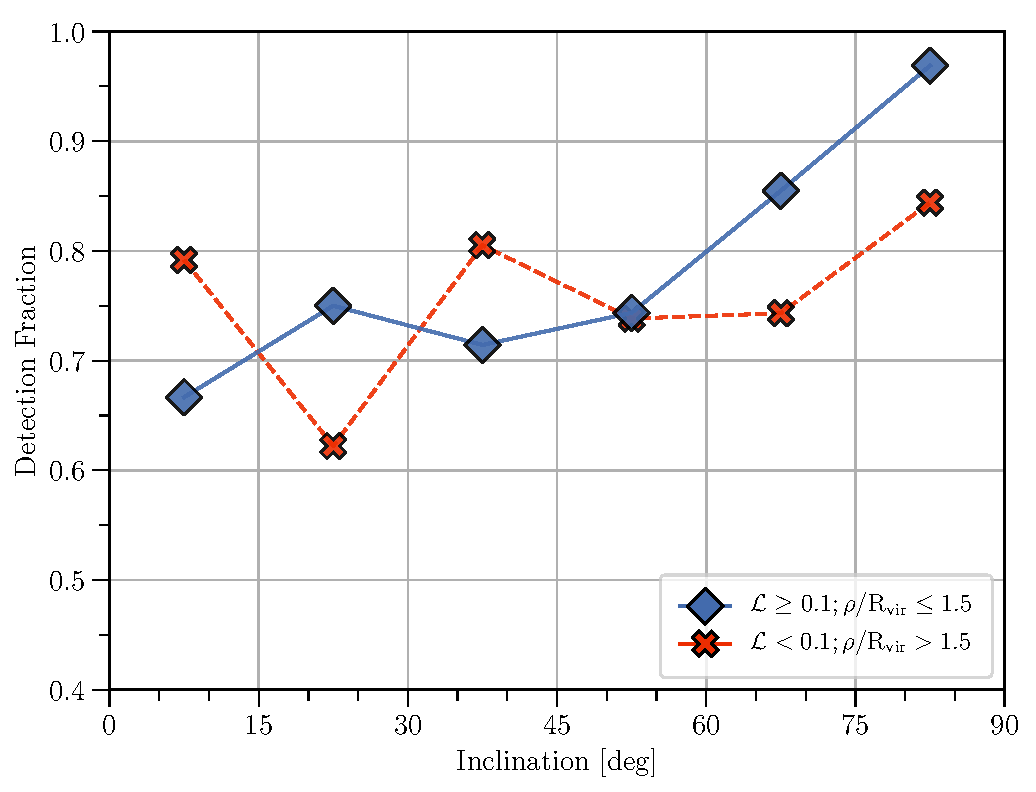
\includegraphics[width=0.49\textwidth]{Chap5/figures/detection_fraction_vs_inc_like_sep15Rvir.pdf}\label{detection_fraction_inc_rvirsep}}
        \caption{\small{(a) The median inclination of galaxies is shown as a function of likelihood $\mathcal{L}$ for both detection (blue-diamonds) and non-detections (red-crosses) of associated absorbers. Detection and non-detection median inclinations are also shown for minimum EW $\rm \ge 200~ m\AA$ absorber equivalent widths by the thinner, semi-transparent lines. (b) The detection fraction plotted directly as a function of inclination for systems inside (blue-diamonds) and outside (orange-pluses) $1.5 \rho / R_{\rm vir}$.}}
        \vspace{0pt}
        \label{detection_fraction_inc_both}
\end{figure}

This result is most easily explained by evoking a non-spherical \HI~galaxy halo. For example, if absorbers are distributed in a perfectly spherical manner around galaxies, then we would expect just as many non-detections as detections at any given galaxy inclination and impact parameter (or likelihood) from a sightline. We do not find this. Thus, the distribution of $\rm Ly\alpha$ absorbers around galaxies must be non-spherical, with a flattened, disk-like $\rm Ly\alpha$ halo fitting the bill nicely. Additionally, Figure \ref{detection_fraction_inc_rvirsep} shows the detection fraction directly as a function of inclination, where we have separated our sample into near ($\rho / R_{\rm vir} \leq 1.5$) and far distributions. Here we can see that the detection fraction is more strongly dependent on inclination for the near systems, where we would expect a stronger effect due to a non-spherical halo.


%\begin{figure}
%\centering
%  \includegraphics[width=0.99\linewidth]{detection_fraction_like_inc_errors_minEW0_200.pdf}
%  \caption{\small{The median inclination of galaxies is shown as a function of likelihood $\mathcal{L}$ for both detection (blue-diamonds) and non-detections (red-crosses) of associated absorbers. Detection and non-detection median inclinations are also shown for EW$\rm = 200~ m\AA$ minimum absorber equivalent widths by the thinner, semi-transparent lines.}}
%\label{detection_fraction_inc}
%\vspace{0pt}
%\end{figure}


%\begin{figure*}
%\centering
%  \subfigure[]{\includegraphics[width=0.49\linewidth]{detection_fraction_impact_inc_median_Lstarcut01-2.pdf}\label{detection_fraction_impact_inc}}
%  \subfigure[]{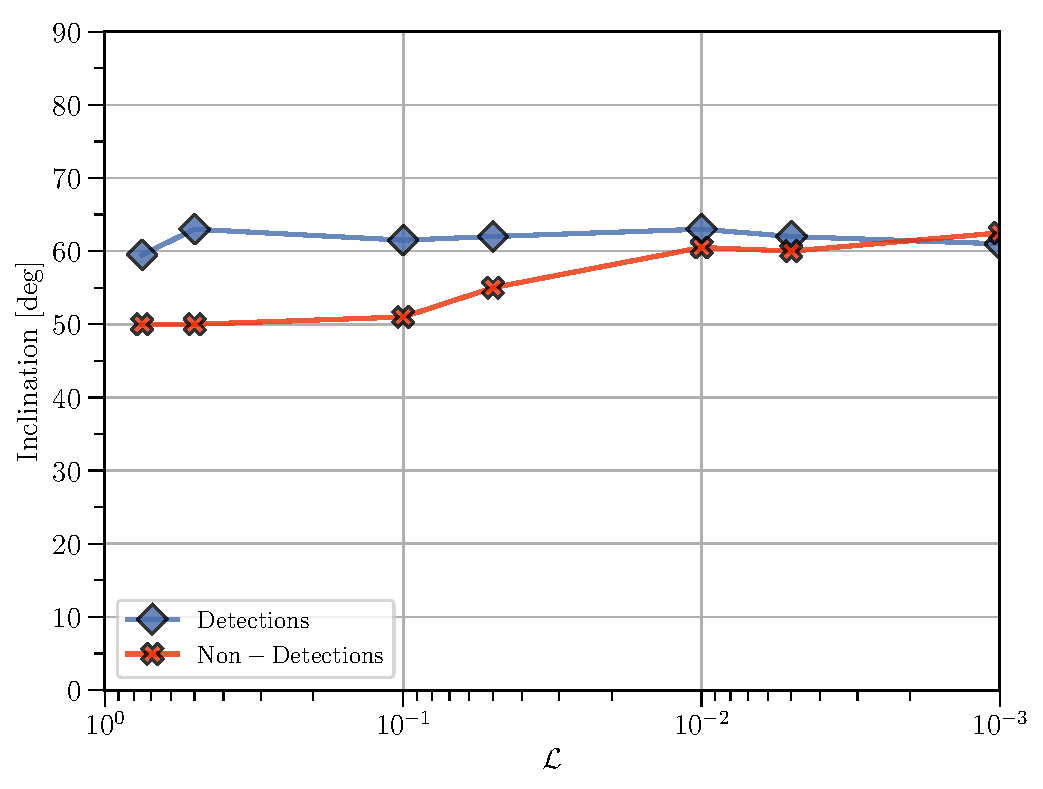
\includegraphics[width=0.49\linewidth]{detection_fraction_likelihood_inc_median_Lstarcut01-2.pdf}\label{detection_fraction_likelihood_inc}}
%  \caption{\small{(a) The median inclination is shown for galaxies at a given impact parameter from a positive (blue-diamonds) or negative (red-crosses) $\rm Ly\alpha$ detection. (b) The median inclination is shown for galaxies at a given $\mathcal{L}$ from a positive (blue-diamonds) or negative (red-crosses) $\rm Ly\alpha$ detection.}}
%  \label{detection_fraction_inclination}
%\vspace{0pt}
%\end{figure*}

\begin{figure}[ht!]
        \centering
        \vspace{0pt}
        \subfigure[]{\includegraphics[width=0.5\textwidth]{Chap5/figures/hist(azimuth)_all_assoc_vs_not_dataset_double.pdf}\label{azimuth_dist}}
        \subfigure[]{\includegraphics[width=0.49\textwidth]{Chap5/figures/detection_fraction_vs_az_like_sep15Rvir.pdf}\label{detection_fraction_az}}
        \caption{\small{(a) The distribution of azimuth angles for the combined $\mathcal{L}-associated$ and $\mathcal{L}-associated-isolated$ subsets is shown in blue, with the $\mathcal{L}-two+$ subset shown in red. (b) The detection fraction plotted as a function of azimuth for systems inside (blue-diamonds) and outside (orange-pluses) $1.5 \rho / R_{\rm vir}$.}}
        \vspace{5pt}
        \label{detection_fraction_inc_both}
\end{figure}


\subsection{Azimuth}
Here we investigate the dependence of $\rm Ly\alpha$ absorber properties on their orientation with respect to the major axis of nearby galaxies. Figure \ref{azimuth_dist} shows the distribution of azimuth angles for systems from the combined $\mathcal{L}-associated$ and $\mathcal{L}-associated-isolated$ subsets in blue, along with the distribution for the $\mathcal{L}-two+$ subset in red. There appears to be a bimodal distribution here, with an excess of absorbers near low (major-axis) and high (minor-axis) azimuth angles. The same is not seen for the 
$\mathcal{L}-two+$ subset, suggesting the presence of other nearby galaxies may be stirring up the $\rm Ly\alpha$ absorbing material in these galaxies' halos. 

Again, we can check the detection fraction as a function of azimuth. Figure \ref{detection_fraction_az} shows this, with the sample split into near ($\rho / R_{\rm vir} \leq 1.5$) and far distributions shown by blue-diamonds and orange-pluses. This detection fraction further backs up the bimodal distribution suggested above, with an elevated detection fraction at both low (major-axis) and high (minor-axis) azimuth angles. The systems beyond $1.5 \rho / R_{\rm vir}$ show a much weaker trend, as expected for systems beyond the direct influence of galaxy halos. This result also agrees with the expectation that gas found near the major axis of a galaxy represents accreting material, while material around the minor axis represents outflows (e.g., \citealt{bordoloi2011, bouche2012, kacprzak2012, bordoloi2014, nielsen2015}). While we cannot tell whether this material is actively inflowing or outflowing, simply the heightened presence of material in the expected regions provides tantalizing hints.

%\begin{figure}
%\centering
%  \includegraphics[width=0.99\linewidth]{hist(azimuth)_all_assoc_vs_not_dataset_double.pdf}
%  \caption{\small{The distribution of azimuth angles for the combined $\mathcal{L}-associated$ and $\mathcal{L}-associated-isolated$ subsets is shown in blue, with the $\mathcal{L}-two+$ subset shown in red.}}
%\label{azimuth_dist}
%\vspace{0pt}
%\end{figure}



\section{Summary}
Here we summarize the results of our study of the $\rm Ly\alpha$ absorber-galaxy connection.

1. The equivalent width of $\rm Ly\alpha$ absorbers depends strongly on environment. The most isolated absorbers are the weakest, with a smooth transition to the strongest absorbers residing very near to multiple galaxies. The separation between the EWs of isolated and non-isolated absorbers is significant at a $> 5\sigma$ level. A similar but far weaker trend is seen for the absorber Doppler $b$-parameters, which will require a dedicated fitting analysis program to overcome blending and saturation issues.

%Likely, this is a result both higher spatial and number density of \HI~cloudlets along the lines of sight near to galaxies. 

2. $\rm Ly\alpha$ absorber EW correlates most strongly with impact parameter when normalized by the associated galaxy virial radii. We find evidence for a lack of strong absorbers within $\sim 0.5 R_{\rm vir}$ of elliptical or S0 type galaxies, but we lack enough systems of these types to report strong limits on this observation.

3. $\rm Ly\alpha$ absorbers with $\rm EW \lesssim 100~m\AA$ are ubiquitous, making up nearly $50\%$ of all $\rm Ly\alpha$ systems in the nearby Universe, and do not correlate strongly with environment ($\sim95\%$ of these weak absorbers are isolated by at least 500 kpc and 400 \kms~from any $L \gtrsim0.1 L^{\**}$ galaxy). 

4. We confirm the \cite{french2017} findings of an overabundance of absorbers located near highly inclined galaxies, and improve the significance of this finding to $4.5\sigma$. We correspondingly find that the $\rm Ly\alpha$ detection fraction increases with increasing galaxy inclination, and that this trend is strongest for systems separated by $1.5 R_{\rm vir}$ or less.

5. We report the first detection of a $\rm Ly\alpha$ azimuth angle dependence, finding that absorbers tend to be associated with galaxy major and minor axes at a $3.3\sigma$ significance. We correspondingly find that the $\rm Ly\alpha$ detection fraction is double peaked around the major and minor axes within $1.5 R_{\rm vir}$, but mostly flat outside of this distance.


%%\begin{eqnarray}
%%	\nonumber
%%	\sigma^2 = \left( \frac{\partial v_{rot}}{\partial \lambda_{obs}} \right)^2 (\Delta \lambda_{obs})^2 + \\
%%	\nonumber
%%	\left(\frac{\partial v_{rot}}{\partial v_{sys}} \right)^2 (\Delta v_{sys})^2 + \\
%%	\left( \frac{\partial v_{rot}}{\partial i} \right)^2 (\Delta i)^2,
%%\end{eqnarray}



\acknowledgements

This research has made use of the NASA/IPAC Extragalactic Database (NED) which is operated by the Jet Propulsion Laboratory, California Institute of Technology, under contract with the National Aeronautics and Space Administration. Based on observations with the NASA/ESA \textit{Hubble Space Telescope}, obtained at the Space Telescope Science Institute (STScI), which is operated by the Association of Universities for Research in Astronomy, Inc., under NASA contract NAS 5-26555. Spectra were retrieved from the Barbara A. Mikulski Archive for Space Telescopes (MAST) at STScI. Over the course of this study, D.M.F. and B.P.W. were supported by grant XXXX

%AST-1108913, awarded by the US National Science Foundation, and by NASA grants \textit{HST}-AR-12842.01-A, \textit{HST}-AR-13893.01-A, and \textit{HST}-GO-14240 (STScI). 

\clearpage

\bibliography{/Users/frenchd/Research/inclination/git_inclination/thesis/DMF_thesis/bib}
\bibliographystyle{thesis}

\clearpage

\chapappendix

\section{Summary of Full QSO Sample and Measurements}
%Here we provide the observation and measurement data for all targets included in this work.

% original table header

%\startlongtable
%\begin{deluxetable}{l c c c c c c c c c}
%\tabletypesize{\scriptsize}
%\tablewidth{0pt}
%\tablecaption{Summary of QSO Sample\label{QSOsample}}
%\tablehead{
%\colhead{Target}  		&  \colhead{R.A.}  	&  \colhead{Dec.}	& \colhead{z} 	&  \colhead{Program} &  \colhead{${T_{\rm exp}}$}	&  \colhead{S/N}			&  \colhead{$v_{\rm Ly\alpha}$}	 &  \colhead{$EW_{\rm Ly\alpha}$}	& \colhead{$b$} \\
%					&  			 	& 		  		& 		     	&				  & \colhead{(ks)}			&  \colhead{(1238 $\rm \AA$)}	&  \colhead{(\kms)}			 &  \colhead{($\rm m\AA$)}		& \colhead{(\kms)} \\
%\colhead{(1)}			& \colhead{(2)}		& \colhead{(3)}		& \colhead{(4)}	& \colhead{(5)}		  & \colhead{(6)}			&  \colhead{(7)}				&  \colhead{(8)}			 	 &  \colhead{(9)}				& \colhead{(10)} }
%\startdata



%\colhead{Target}  		&  \colhead{R.A.}  	&  \colhead{Dec.}	& \colhead{z} 	&  \colhead{Program} &  \colhead{${T_{\rm exp}}$}	&  \colhead{S/N}			&  \colhead{$v_{\rm Ly\alpha}$}	 &  \colhead{$EW_{\rm Ly\alpha}$}	& \colhead{$b$} \\
%					&  			 	& 		  		& 		     	&				  & \colhead{(ks)}			&  \colhead{(1238 $\rm \AA$)}	&  \colhead{(\kms)}			 &  \colhead{($\rm m\AA$)}		& \colhead{(\kms)} \\
%\colhead{(1)}			& \colhead{(2)}		& \colhead{(3)}		& \colhead{(4)}	& \colhead{(5)}		  & \colhead{(6)}			&  \colhead{(7)}				&  \colhead{(8)}			 	 &  \colhead{(9)}				& \colhead{(10)} }



\begin{landscape}

% Change the footnote style to lowercase letters
\renewcommand{\thefootnote}{\alph{footnote}}

\scriptsize
\begin{center}
\begin{longtable}{l c c c c c c c c c}
\caption[Summary of Full QSO Sample and Measurements]{Summary of Full QSO Sample and Measurements} \label{QSOsample} \\
\hline \hline \\[-2ex]
  \multicolumn{1}{c}{Target} & 
  \multicolumn{1}{c}{R.A.} &
  \multicolumn{1}{c}{Dec.} &
  \multicolumn{1}{c}{z} &
  \multicolumn{1}{c}{Program} &
  \multicolumn{1}{c}{${T_{\rm exp}}$\tablenotemark{a}} &
  \multicolumn{1}{c}{S/N} &
  \multicolumn{1}{c}{$v_{\rm Ly\alpha}$} &
  \multicolumn{1}{c}{$EW_{\rm Ly\alpha}$} &
  \multicolumn{1}{c}{$b$} \\
  
  % Units
  \multicolumn{1}{c}{} & 
  \multicolumn{1}{c}{(J2000)} &
  \multicolumn{1}{c}{(J2000)} &
  \multicolumn{1}{c}{} &
  \multicolumn{1}{c}{} &
  \multicolumn{1}{c}{(ks)}&
  \multicolumn{1}{c}{(1238 $\rm \AA$)} &
  \multicolumn{1}{c}{(\kms)} &
  \multicolumn{1}{c}{($\rm m\AA$)} &
  \multicolumn{1}{c}{(\kms)} \\
  
  % column numbers
  \multicolumn{1}{c}{(1)} & 
  \multicolumn{1}{c}{(2)} &
  \multicolumn{1}{c}{(3)} &
  \multicolumn{1}{c}{(4)} &
  \multicolumn{1}{c}{(5)} &
  \multicolumn{1}{c}{(6)} &
  \multicolumn{1}{c}{(7)} &
  \multicolumn{1}{c}{(8)} &
  \multicolumn{1}{c}{(9)} &
  \multicolumn{1}{c}{(10)} \\[0.5ex] \hline \\[-1.8ex]
\endfirsthead

% Second page
\multicolumn{10}{c}{{\tablename} \thetable{} -- Continued} \\[0.5ex]
\hline \hline \\[-2ex]
  \multicolumn{1}{c}{Target} & 
  \multicolumn{1}{c}{R.A.} &
  \multicolumn{1}{c}{Dec.} &
  \multicolumn{1}{c}{z} &
  \multicolumn{1}{c}{Program} &
  \multicolumn{1}{c}{${T_{\rm exp}}$\tablenotemark{a}} &
  \multicolumn{1}{c}{S/N} &
  \multicolumn{1}{c}{$v_{\rm Ly\alpha}$} &
  \multicolumn{1}{c}{$EW_{\rm Ly\alpha}$} &
  \multicolumn{1}{c}{$b$} \\
  
  % Units
  \multicolumn{1}{c}{} & 
  \multicolumn{1}{c}{(J2000)} &
  \multicolumn{1}{c}{(J2000)} &
  \multicolumn{1}{c}{} &
  \multicolumn{1}{c}{} &
  \multicolumn{1}{c}{(ks)}&
  \multicolumn{1}{c}{(1238 $\rm \AA$)} &
  \multicolumn{1}{c}{(\kms)} &
  \multicolumn{1}{c}{($\rm m\AA$)} &
  \multicolumn{1}{c}{(\kms)} \\
  
  % column numbers
  \multicolumn{1}{c}{(1)} & 
  \multicolumn{1}{c}{(2)} &
  \multicolumn{1}{c}{(3)} &
  \multicolumn{1}{c}{(4)} &
  \multicolumn{1}{c}{(5)} &
  \multicolumn{1}{c}{(6)} &
  \multicolumn{1}{c}{(7)} &
  \multicolumn{1}{c}{(8)} &
  \multicolumn{1}{c}{(9)} &
  \multicolumn{1}{c}{(10)} \\[0.5ex] \hline \\[-1.8ex]
  \endhead

\multicolumn{10}{l}{{Continued on Next Page\ldots}} \\
\endfoot

\\[-1.8ex] \hline \hline
\endlastfoot
1H0419-577  &              04 26 00.8  &         $-$57 12 01.0  &       0.10400  & 11686  &   20429  &      58.4  &      1075.0  &  249.0  &  28.2  \\
1H0419-577  &              04 26 00.8  &         $-$57 12 01.0  &       0.10400  & 11686  &   20429  &      58.4  &      1123.0  &  269.0  &  26.8  \\
1H0419-577  &              04 26 00.8  &         $-$57 12 01.0  &       0.10400  & 11686  &   20429  &      58.4  &      1188.0  &  240.0  &  29.7  \\
1H0419-577  &              04 26 00.8  &         $-$57 12 01.0  &       0.10400  & 11686  &   20429  &      58.4  &      1264.0  &  91.0  &   32.5  \\
1H0419-577  &              04 26 00.8  &         $-$57 12 01.0  &       0.10400  & 11686  &   20429  &      58.4  &      2020.0  &  9.0  &    17.5  \\
1H0419-577  &              04 26 00.8  &         $-$57 12 01.0  &       0.10400  & 11686  &   20429  &      58.4  &      7801.0  &  122.0  &  43.9  \\
1H0419-577  &              04 26 00.8  &         $-$57 12 01.0  &       0.10400  & 11686  &   20429  &      58.4  &      8819.0  &  39.0  &   30.4  \\
1H0419-577  &              04 26 00.8  &         $-$57 12 01.0  &       0.10400  & 11686  &   20429  &      58.4  &      9962.0  &  34.0  &   23.3  \\
1H0717+714  &              07 21 53.5  &         $+$71 20 36.0  &       0.23149  & 12025  &   6000  &       23.4  &      2873.0  &  349.0  &  58.3  \\
1H0717+714  &              07 21 53.5  &         $+$71 20 36.0  &       0.23149  & 12025  &   6000  &       23.4  &      2988.0  &  33.0  &   22.7  \\
1H0717+714  &              07 21 53.5  &         $+$71 20 36.0  &       0.23149  & 12025  &   6000  &       23.4  &      3840.0  &  39.0  &   38.2  \\
1H0717+714  &              07 21 53.5  &         $+$71 20 36.0  &       0.23149  & 12025  &   6000  &       23.4  &      5283.0  &  51.0  &   49.9  \\
1H0717+714  &              07 21 53.5  &         $+$71 20 36.0  &       0.23149  & 12025  &   6000  &       23.4  &      6271.0  &  167.0  &  44.4  \\
1H0717+714  &              07 21 53.5  &         $+$71 20 36.0  &       0.23149  & 12025  &   6000  &       23.4  &      6595.0  &  64.0  &   38.6  \\
1H0717+714  &              07 21 53.5  &         $+$71 20 36.0  &       0.23149  & 12025  &   6000  &       23.4  &      7799.0  &  52.0  &   27.9  \\
1H1613-097  &              16 15 19.1  &         $-$09 36 13.0  &       0.06496  & 13448  &   4833  &       12.9  &      3678.0  &  39.0  &   17.5  \\
1H1613-097  &              16 15 19.1  &         $-$09 36 13.0  &       0.06496  & 13448  &   4833  &       12.9  &      5259.0  &  55.0  &   19.6  \\
1H1613-097  &              16 15 19.1  &         $-$09 36 13.0  &       0.06496  & 13448  &   4833  &       12.9  &      7326.0  &  212.0  &  42.9  \\
1H1613-097  &              16 15 19.1  &         $-$09 36 13.0  &       0.06496  & 13448  &   4833  &       12.9  &      8204.0  &  339.0  &  40.5  \\
2E1530+1511  &             15 33 14.3  &         $+$15 01 02.0  &       0.09000  & 14071  &   9348  &       9.1  &       1795.0  &  507.0  &  62.7  \\
2E1530+1511  &             15 33 14.3  &         $+$15 01 02.0  &       0.09000  & 14071  &   9348  &       9.1  &       1953.0  &  137.0  &  26.8  \\
2dFGRS\_S393Z082  &        02 45 00.8  &         $-$30 07 23.0  &       0.33921  & 12988  &   17668  &      11.5  &      1236.0  &  563.0  &  60.9  \\
2dFGRS\_S393Z082  &        02 45 00.8  &         $-$30 07 23.0  &       0.33921  & 12988  &   17668  &      11.5  &      3011.0  &  48.0  &   19.2  \\
2dFGRS\_S393Z082  &        02 45 00.8  &         $-$30 07 23.0  &       0.33921  & 12988  &   17668  &      11.5  &      3759.0  &  58.0  &   40.2  \\
2dFGRS\_S393Z082  &        02 45 00.8  &         $-$30 07 23.0  &       0.33921  & 12988  &   17668  &      11.5  &      4042.0  &  36.0  &   17.9  \\
3C232  &                   09 58 20.9  &         $+$32 24 02.0  &       0.53060  & P107  &    11000  &      11.4  &      1467.0  &  3822.0  & 386.5  \\
3C232  &                   09 58 20.9  &         $+$32 24 02.0  &       0.53060  & P107  &    11000  &      11.4  &      1408.0  &  2092.0  & 212.8  \\
3C232  &                   09 58 20.9  &         $+$32 24 02.0  &       0.53060  & P107  &    11000  &      11.4  &      1510.0  &  700.0  &  70.3  \\
3C232  &                   09 58 20.9  &         $+$32 24 02.0  &       0.53060  & P107  &    11000  &      11.4  &      1641.0  &  1635.0  & 191.9  \\
3C232  &                   09 58 20.9  &         $+$32 24 02.0  &       0.53060  & P107  &    11000  &      11.4  &      4528.0  &  128.0  &  76.8  \\
3C249.1  &                 11 04 13.8  &         $+$76 58 58.0  &       0.31150  & 4939  &    19157  &      9.1  &       1860.0  &  43.0  &   25.6  \\
3C249.1  &                 11 04 13.8  &         $+$76 58 58.0  &       0.31150  & 4939  &    19157  &      9.1  &       6674.0  &  249.0  &  53.9  \\
3C249.1  &                 11 04 13.8  &         $+$76 58 58.0  &       0.31150  & 4939  &    19157  &      9.1  &       7815.0  &  287.0  &  44.4  \\
3C249.1  &                 11 04 13.8  &         $+$76 58 58.0  &       0.31150  & 4939  &    19157  &      9.1  &       8383.0  &  294.0  &  39.4  \\
3C263  &                   11 39 57.0  &         $+$65 47 51.0  &       0.64600  & 11541  &   15360  &      35.7  &      2175.0  &  52.0  &   29.3  \\
3C263  &                   11 39 57.0  &         $+$65 47 51.0  &       0.64600  & 11541  &   15360  &      35.7  &      3910.0  &  12.0  &   17.1  \\
3C263  &                   11 39 57.0  &         $+$65 47 51.0  &       0.64600  & 11541  &   15360  &      35.7  &      8954.0  &  42.0  &   23.6  \\
3C263  &                   11 39 57.0  &         $+$65 47 51.0  &       0.64600  & 11541  &   15360  &      35.7  &      9651.0  &  13.0  &   14.8  \\
3C263  &                   11 39 57.0  &         $+$65 47 51.0  &       0.64600  & 11541  &   15360  &      35.7  &      9764.0  &  134.0  &  44.6  \\
3C273.0  &                 12 29 06.7  &         $+$02 03 09.0  &       0.15834  & 12038  &   4002  &       63.2  &      1013.0  &  382.0  &  44.3  \\
3C273.0  &                 12 29 06.7  &         $+$02 03 09.0  &       0.15834  & 12038  &   4002  &       63.2  &      1580.0  &  369.0  &  42.0  \\
3C273.0  &                 12 29 06.7  &         $+$02 03 09.0  &       0.15834  & 12038  &   4002  &       63.2  &      2156.0  &  42.0  &   57.9  \\
3C273.0  &                 12 29 06.7  &         $+$02 03 09.0  &       0.15834  & 12038  &   4002  &       63.2  &      2267.0  &  27.0  &   36.1  \\
3C273.0  &                 12 29 06.7  &         $+$02 03 09.0  &       0.15834  & 12038  &   4002  &       63.2  &      7857.0  &  42.0  &   30.6  \\
3C273.0  &                 12 29 06.7  &         $+$02 03 09.0  &       0.15834  & 12038  &   4002  &       63.2  &      8828.0  &  138.0  &  49.9  \\
3C273.0  &                 12 29 06.7  &         $+$02 03 09.0  &       0.15834  & 12038  &   4002  &       63.2  &      9835.0  &  39.0  &   30.0  \\
3C323.1  &                 15 47 43.6  &         $+$20 52 16.0  &       0.26430  & 13398  &   9841  &       24.2  &      2133.0  &  240.0  &  50.1  \\
3C323.1  &                 15 47 43.6  &         $+$20 52 16.0  &       0.26430  & 13398  &   9841  &       24.2  &      4222.0  &  290.0  &  46.1  \\
3C323.1  &                 15 47 43.6  &         $+$20 52 16.0  &       0.26430  & 13398  &   9841  &       24.2  &      4416.0  &  138.0  &  43.2  \\
3C323.1  &                 15 47 43.6  &         $+$20 52 16.0  &       0.26430  & 13398  &   9841  &       24.2  &      4749.0  &  55.0  &   35.9  \\
3C323.1  &                 15 47 43.6  &         $+$20 52 16.0  &       0.26430  & 13398  &   9841  &       24.2  &      6309.0  &  39.0  &   36.3  \\
3C351.0  &                 17 04 41.6  &         $+$60 44 29.0  &       0.37194  & P108  &    142000  &     8.9  &       3462.0  &  147.0  &  49.0  \\
3C351.0  &                 17 04 41.6  &         $+$60 44 29.0  &       0.37194  & P108  &    142000  &     8.9  &       3597.0  &  195.0  &  39.3  \\
3C351.0  &                 17 04 41.6  &         $+$60 44 29.0  &       0.37194  & P108  &    142000  &     8.9  &       5078.0  &  81.0  &   33.7  \\
3C351.0  &                 17 04 41.6  &         $+$60 44 29.0  &       0.37194  & P108  &    142000  &     8.9  &       5175.0  &  207.0  &  44.7  \\
3C351.0  &                 17 04 41.6  &         $+$60 44 29.0  &       0.37194  & P108  &    142000  &     8.9  &       7172.0  &  60.0  &   27.6  \\
3C351.0  &                 17 04 41.6  &         $+$60 44 29.0  &       0.37194  & P108  &    142000  &     8.9  &       8382.0  &  29.0  &   18.2  \\
3C57  &                    02 01 57.1  &         $-$11 32 34.0  &       0.66900  & 12038  &   10963  &      22.8  &      4581.0  &  35.0  &   20.9  \\
3C57  &                    02 01 57.1  &         $-$11 32 34.0  &       0.66900  & 12038  &   10963  &      22.8  &      5370.0  &  29.0  &   26.5  \\
3C57  &                    02 01 57.1  &         $-$11 32 34.0  &       0.66900  & 12038  &   10963  &      22.8  &      6685.0  &  32.0  &   20.2  \\
3C57  &                    02 01 57.1  &         $-$11 32 34.0  &       0.66900  & 12038  &   10963  &      22.8  &      8113.0  &  13.0  &   13.8  \\
3C66A  &                   02 22 39.6  &         $+$43 02 08.0  &       0.44400  & 12612  &   12600  &      25.9  &      4301.0  &  24.0  &   16.6  \\
3C66A  &                   02 22 39.6  &         $+$43 02 08.0  &       0.44400  & 12612  &   12600  &      25.9  &      8188.0  &  113.0  &  29.5  \\
4C25.01  &                 00 19 39.8  &         $+$26 02 52.0  &       0.28400  & 14268  &   3739  &       19.6  &      996.0  &   95.0  &   24.0  \\
4C25.01  &                 00 19 39.8  &         $+$26 02 52.0  &       0.28400  & 14268  &   3739  &       19.6  &      3351.0  &  55.0  &   39.0  \\
4C25.01  &                 00 19 39.8  &         $+$26 02 52.0  &       0.28400  & 14268  &   3739  &       19.6  &      9450.0  &  105.0  &  24.4  \\
CSO1161  &                 11 20 07.4  &         $+$42 35 51.0  &       0.22706  & 14772  &   4767  &       10  &        3144.0  &  164.0  &  39.3  \\
CSO1161  &                 11 20 07.4  &         $+$42 35 51.0  &       0.22706  & 14772  &   4767  &       10  &        3784.0  &  69.0  &   40.4  \\
CSO1161  &                 11 20 07.4  &         $+$42 35 51.0  &       0.22706  & 14772  &   4767  &       10  &        7322.0  &  253.0  &  48.0  \\
CSO1161  &                 11 20 07.4  &         $+$42 35 51.0  &       0.22706  & 14772  &   4767  &       10  &        7766.0  &  337.0  &  50.8  \\
CSO1161  &                 11 20 07.4  &         $+$42 35 51.0  &       0.22706  & 14772  &   4767  &       10  &        8827.0  &  187.0  &  55.0  \\
CSO1161  &                 11 20 07.4  &         $+$42 35 51.0  &       0.22706  & 14772  &   4767  &       10  &        8942.0  &  233.0  &  78.5  \\
CSO1208  &                 11 40 48.0  &         $+$46 22 05.0  &       0.11439  & 14729  &   7228  &       7.7  &       731.0  &   470.0  &  54.2  \\
CSO1208  &                 11 40 48.0  &         $+$46 22 05.0  &       0.11439  & 14729  &   7228  &       7.7  &       874.0  &   506.0  &  58.7  \\
CSO1208  &                 11 40 48.0  &         $+$46 22 05.0  &       0.11439  & 14729  &   7228  &       7.7  &       5339.0  &  129.0  &  25.5  \\
CSO1208  &                 11 40 48.0  &         $+$46 22 05.0  &       0.11439  & 14729  &   7228  &       7.7  &       6852.0  &  143.0  &  40.1  \\
CSO1208  &                 11 40 48.0  &         $+$46 22 05.0  &       0.11439  & 14729  &   7228  &       7.7  &       7281.0  &  83.0  &   23.8  \\
CSO1208  &                 11 40 48.0  &         $+$46 22 05.0  &       0.11439  & 14729  &   7228  &       7.7  &       7426.0  &  102.0  &  21.3  \\
CSO1245  &                 11 56 30.1  &         $+$42 52 54.0  &       1.01545  & 14772  &   4821  &       11  &        1178.0  &  74.0  &   23.7  \\
CSO1245  &                 11 56 30.1  &         $+$42 52 54.0  &       1.01545  & 14772  &   4821  &       11  &        3228.0  &  98.0  &   28.5  \\
CSO1245  &                 11 56 30.1  &         $+$42 52 54.0  &       1.01545  & 14772  &   4821  &       11  &        5590.0  &  33.0  &   17.9  \\
CSO1245  &                 11 56 30.1  &         $+$42 52 54.0  &       1.01545  & 14772  &   4821  &       11  &        7077.0  &  177.0  &  27.1  \\
CSO1245  &                 11 56 30.1  &         $+$42 52 54.0  &       1.01545  & 14772  &   4821  &       11  &        7139.0  &  204.0  &  24.9  \\
CSO295  &                  10 52 05.5  &         $+$36 40 40.0  &       0.60999  & 14772  &   2174  &       11.9  &      600.0  &   568.0  &  64.1  \\
CSO295  &                  10 52 05.5  &         $+$36 40 40.0  &       0.60999  & 14772  &   2174  &       11.9  &      662.0  &   585.0  &  77.5  \\
CSO295  &                  10 52 05.5  &         $+$36 40 40.0  &       0.60999  & 14772  &   2174  &       11.9  &      5658.0  &  117.0  &  38.0  \\
CSO295  &                  10 52 05.5  &         $+$36 40 40.0  &       0.60999  & 14772  &   2174  &       11.9  &      7640.0  &  352.0  &  68.3  \\
CSO295  &                  10 52 05.5  &         $+$36 40 40.0  &       0.60999  & 14772  &   2174  &       11.9  &      7774.0  &  150.0  &  31.4  \\
CSO395  &                  12 11 14.6  &         $+$36 57 39.0  &       0.17109  & 12248  &   3012  &       13.4  &      961.0  &   204.0  &  31.8  \\
CSO395  &                  12 11 14.6  &         $+$36 57 39.0  &       0.17109  & 12248  &   3012  &       13.4  &      1022.0  &  355.0  &  42.8  \\
CSO395  &                  12 11 14.6  &         $+$36 57 39.0  &       0.17109  & 12248  &   3012  &       13.4  &      961.0  &   204.0  &  31.8  \\
CSO395  &                  12 11 14.6  &         $+$36 57 39.0  &       0.17109  & 12248  &   3012  &       13.4  &      1022.0  &  355.0  &  42.8  \\
CTS487  &                  23 22 11.0  &         $-$34 47 57.0  &       0.42000  & 13448  &   8061  &       19.6  &      2750.0  &  80.0  &   44.4  \\
ESO141-G55  &              19 21 14.3  &         $-$58 40 13.0  &       0.03600  & 12936  &   2178  &       37.1  &      2140.0  &  50.0  &   33.0  \\
ESO141-G55  &              19 21 14.3  &         $-$58 40 13.0  &       0.03600  & 12936  &   2178  &       37.1  &      5283.0  &  26.0  &   35.4  \\
ESO265-G23  &              11 20 47.9  &         $-$43 15 51.0  &       0.05600  & 12275  &   1983  &       14.7  &      8470.0  &  252.0  &  44.3  \\
ESO350-IG38  &             00 36 52.9  &         $-$33 33 19.0  &       0.02060  & 13017  &   7596  &       17.8  &      1608.0  &  391.0  &  82.7  \\
FAIRALL9  &                01 23 45.8  &         $-$58 48 21.0  &       0.04702  & 12604  &   4960  &       41.3  &      9515.0  &  73.0  &   34.0  \\
FBQSJ0751+2919  &          07 51 12.3  &         $+$29 19 38.0  &       0.92240  & 11741  &   16531  &      27.5  &      3525.0  &  26.0  &   17.6  \\
FBQSJ0751+2919  &          07 51 12.3  &         $+$29 19 38.0  &       0.92240  & 11741  &   16531  &      27.5  &      3560.0  &  41.0  &   23.8  \\
FBQSJ0751+2919  &          07 51 12.3  &         $+$29 19 38.0  &       0.92240  & 11741  &   16531  &      27.5  &      3635.0  &  55.0  &   20.8  \\
FBQSJ0751+2919  &          07 51 12.3  &         $+$29 19 38.0  &       0.92240  & 11741  &   16531  &      27.5  &      3677.0  &  44.0  &   23.9  \\
FBQSJ0751+2919  &          07 51 12.3  &         $+$29 19 38.0  &       0.92240  & 11741  &   16531  &      27.5  &      6297.0  &  23.0  &   20.9  \\
FBQSJ0751+2919  &          07 51 12.3  &         $+$29 19 38.0  &       0.92240  & 11741  &   16531  &      27.5  &      7380.0  &  22.0  &   24.8  \\
FBQSJ0751+2919  &          07 51 12.3  &         $+$29 19 38.0  &       0.92240  & 11741  &   16531  &      27.5  &      8020.0  &  300.0  &  39.5  \\
FBQSJ0908+3246  &          09 08 38.8  &         $+$32 46 20.0  &       0.25989  & 14240  &   7430  &       10  &        1915.0  &  202.0  &  27.1  \\
FBQSJ0908+3246  &          09 08 38.8  &         $+$32 46 20.0  &       0.25989  & 14240  &   7430  &       10  &        1982.0  &  230.0  &  42.1  \\
FBQSJ0908+3246  &          09 08 38.8  &         $+$32 46 20.0  &       0.25989  & 14240  &   7430  &       10  &        4287.0  &  367.0  &  56.4  \\
FBQSJ0908+3246  &          09 08 38.8  &         $+$32 46 20.0  &       0.25989  & 14240  &   7430  &       10  &        7926.0  &  95.0  &   40.1  \\
FBQSJ1134+2555  &          11 34 57.6  &         $+$25 55 28.0  &       0.70994  & 12248  &   4235  &       9.2  &       3070.0  &  106.0  &  32.3  \\
FBQSJ1134+2555  &          11 34 57.6  &         $+$25 55 28.0  &       0.70994  & 12248  &   4235  &       9.2  &       6343.0  &  86.0  &   31.0  \\
FBQSJ1134+2555  &          11 34 57.6  &         $+$25 55 28.0  &       0.70994  & 12248  &   4235  &       9.2  &       9552.0  &  636.0  &  71.2  \\
FBQSJ1353+3620  &          13 53 26.0  &         $+$36 20 49.0  &       0.28504  & 13444  &   4777  &       13.9  &      2560.0  &  50.0  &   38.1  \\
FBQSJ1353+3620  &          13 53 26.0  &         $+$36 20 49.0  &       0.28504  & 13444  &   4777  &       13.9  &      5464.0  &  86.0  &   43.2  \\
FBQSJ1353+3620  &          13 53 26.0  &         $+$36 20 49.0  &       0.28504  & 13444  &   4777  &       13.9  &      6174.0  &  117.0  &  43.1  \\
FBQSJ1353+3620  &          13 53 26.0  &         $+$36 20 49.0  &       0.28504  & 13444  &   4777  &       13.9  &      6587.0  &  395.0  &  67.3  \\
FBQSJ1431+2442  &          14 31 25.8  &         $+$24 42 20.0  &       0.40691  & 12603  &   16501  &      17.5  &      2241.0  &  28.0  &   29.2  \\
FBQSJ1431+2442  &          14 31 25.8  &         $+$24 42 20.0  &       0.40691  & 12603  &   16501  &      17.5  &      2804.0  &  29.0  &   18.3  \\
FBQSJ1431+2442  &          14 31 25.8  &         $+$24 42 20.0  &       0.40691  & 12603  &   16501  &      17.5  &      4861.0  &  41.0  &   26.9  \\
FBQSJ1431+2442  &          14 31 25.8  &         $+$24 42 20.0  &       0.40691  & 12603  &   16501  &      17.5  &      5662.0  &  94.0  &   50.5  \\
FBQSJ1431+2442  &          14 31 25.8  &         $+$24 42 20.0  &       0.40691  & 12603  &   16501  &      17.5  &      6542.0  &  33.0  &   13.5  \\
FBQSJ1431+2442  &          14 31 25.8  &         $+$24 42 20.0  &       0.40691  & 12603  &   16501  &      17.5  &      6623.0  &  285.0  &  47.0  \\
FBS0150+396  &             01 53 06.7  &         $+$39 55 45.0  &       0.21190  & 14268  &   5022  &       9  &         5812.0  &  281.0  &  43.6  \\
FBS0150+396  &             01 53 06.7  &         $+$39 55 45.0  &       0.21190  & 14268  &   5022  &       9  &         7270.0  &  74.0  &   49.0  \\
FBS1526+659  &             15 27 28.5  &         $+$65 48 10.0  &       0.34500  & 12276  &   2032  &       10.8  &      7776.0  &  308.0  &  38.3  \\
FBS1526+659  &             15 27 28.5  &         $+$65 48 10.0  &       0.34500  & 12276  &   2032  &       10.8  &      8975.0  &  466.0  &  50.8  \\
H1101-232  &               11 03 37.7  &         $-$23 29 31.0  &       0.18600  & 12025  &   13341  &      16.4  &      1182.0  &  635.0  &  69.5  \\
H1101-232  &               11 03 37.7  &         $-$23 29 31.0  &       0.18600  & 12025  &   13341  &      16.4  &      2117.0  &  46.0  &   34.6  \\
H1101-232  &               11 03 37.7  &         $-$23 29 31.0  &       0.18600  & 12025  &   13341  &      16.4  &      3565.0  &  563.0  &  56.1  \\
H1101-232  &               11 03 37.7  &         $-$23 29 31.0  &       0.18600  & 12025  &   13341  &      16.4  &      5835.0  &  38.0  &   29.4  \\
H1101-232  &               11 03 37.7  &         $-$23 29 31.0  &       0.18600  & 12025  &   13341  &      16.4  &      8860.0  &  37.0  &   21.7  \\
H1821+643  &               18 21 57.2  &         $+$64 20 36.0  &       0.29700  & 11484  &   12039  &      40.2  &      1100.0  &  33.0  &   26.1  \\
H1821+643  &               18 21 57.2  &         $+$64 20 36.0  &       0.29700  & 11484  &   12039  &      40.2  &      2818.0  &  40.0  &   49.5  \\
H1821+643  &               18 21 57.2  &         $+$64 20 36.0  &       0.29700  & 11484  &   12039  &      40.2  &      7313.0  &  338.0  &  42.6  \\
H1821+643  &               18 21 57.2  &         $+$64 20 36.0  &       0.29700  & 11484  &   12039  &      40.2  &      7931.0  &  69.0  &   47.1  \\
HE0056-3622  &             00 58 37.4  &         $-$36 06 05.0  &       0.16414  & 12604  &   4959  &       27.7  &      3462.0  &  227.0  &  49.2  \\
HE0056-3622  &             00 58 37.4  &         $-$36 06 05.0  &       0.16414  & 12604  &   4959  &       27.7  &      5127.0  &  95.0  &   31.0  \\
HE0056-3622  &             00 58 37.4  &         $-$36 06 05.0  &       0.16414  & 12604  &   4959  &       27.7  &      8455.0  &  120.0  &  38.2  \\
HE0153-4520  &             01 55 13.2  &         $-$45 06 12.0  &       0.45100  & 11541  &   5228  &       29.8  &      6311.0  &  17.0  &   17.9  \\
HE0153-4520  &             01 55 13.2  &         $-$45 06 12.0  &       0.45100  & 11541  &   5228  &       29.8  &      7101.0  &  31.0  &   28.2  \\
HE0226-4110  &             02 28 15.2  &         $-$40 57 16.0  &       0.49500  & 11541  &   6775  &       27.7  &      3644.0  &  25.0  &   34.5  \\
HE0226-4110  &             02 28 15.2  &         $-$40 57 16.0  &       0.49500  & 11541  &   6775  &       27.7  &      5233.0  &  72.0  &   33.1  \\
HE0226-4110  &             02 28 15.2  &         $-$40 57 16.0  &       0.49500  & 11541  &   6775  &       27.7  &      7592.0  &  35.0  &   38.6  \\
HE0226-4110  &             02 28 15.2  &         $-$40 57 16.0  &       0.49500  & 11541  &   6775  &       27.7  &      8027.0  &  102.0  &  43.4  \\
HE0226-4110  &             02 28 15.2  &         $-$40 57 16.0  &       0.49500  & 11541  &   6775  &       27.7  &      9292.0  &  13.0  &   24.2  \\
HE0241-3043  &             02 43 37.7  &         $-$30 30 48.0  &       0.66929  & 12988  &   6972  &       17.3  &      1219.0  &  77.0  &   23.0  \\
HE0241-3043  &             02 43 37.7  &         $-$30 30 48.0  &       0.66929  & 12988  &   6972  &       17.3  &      1310.0  &  178.0  &  32.7  \\
HE0241-3043  &             02 43 37.7  &         $-$30 30 48.0  &       0.66929  & 12988  &   6972  &       17.3  &      2299.0  &  65.0  &   45.4  \\
HE0241-3043  &             02 43 37.7  &         $-$30 30 48.0  &       0.66929  & 12988  &   6972  &       17.3  &      2624.0  &  28.0  &   20.8  \\
HE0241-3043  &             02 43 37.7  &         $-$30 30 48.0  &       0.66929  & 12988  &   6972  &       17.3  &      3096.0  &  34.0  &   33.3  \\
HE0241-3043  &             02 43 37.7  &         $-$30 30 48.0  &       0.66929  & 12988  &   6972  &       17.3  &      4979.0  &  53.0  &   23.3  \\
HE0241-3043  &             02 43 37.7  &         $-$30 30 48.0  &       0.66929  & 12988  &   6972  &       17.3  &      5681.0  &  29.0  &   13.9  \\
HE0241-3043  &             02 43 37.7  &         $-$30 30 48.0  &       0.66929  & 12988  &   6972  &       17.3  &      7145.0  &  55.0  &   30.7  \\
HE0241-3043  &             02 43 37.7  &         $-$30 30 48.0  &       0.66929  & 12988  &   6972  &       17.3  &      7487.0  &  57.0  &   41.1  \\
HE0241-3043  &             02 43 37.7  &         $-$30 30 48.0  &       0.66929  & 12988  &   6972  &       17.3  &      9881.0  &  47.0  &   30.5  \\
HE0340-2703  &             03 42 20.6  &         $-$26 53 59.0  &       0.28300  & 9378  &    4895  &       8.5  &       1345.0  &  268.0  &  48.1  \\
HE0340-2703  &             03 42 20.6  &         $-$26 53 59.0  &       0.28300  & 9378  &    4895  &       8.5  &       1766.0  &  374.0  &  57.7  \\
HE0340-2703  &             03 42 20.6  &         $-$26 53 59.0  &       0.28300  & 9378  &    4895  &       8.5  &       4083.0  &  194.0  &  36.6  \\
HE0429-5343  &             04 30 40.0  &         $-$53 36 56.0  &       0.04001  & 12275  &   2067  &       15.1  &      1167.0  &  79.0  &   25.8  \\
HE0429-5343  &             04 30 40.0  &         $-$53 36 56.0  &       0.04001  & 12275  &   2067  &       15.1  &      1358.0  &  136.0  &  57.8  \\
HE0429-5343  &             04 30 40.0  &         $-$53 36 56.0  &       0.04001  & 12275  &   2067  &       15.1  &      3949.0  &  158.0  &  31.0  \\
HE0429-5343  &             04 30 40.0  &         $-$53 36 56.0  &       0.04001  & 12275  &   2067  &       15.1  &      4951.0  &  134.0  &  34.1  \\
HE0429-5343  &             04 30 40.0  &         $-$53 36 56.0  &       0.04001  & 12275  &   2067  &       15.1  &      5638.0  &  92.0  &   34.7  \\
HE0429-5343  &             04 30 40.0  &         $-$53 36 56.0  &       0.04001  & 12275  &   2067  &       15.1  &      8953.0  &  555.0  &  61.1  \\
HE0435-5304  &             04 36 50.8  &         $-$52 58 49.0  &       0.42616  & 11520  &   8372  &       13.3  &      1512.0  &  229.0  &  41.0  \\
HE0435-5304  &             04 36 50.8  &         $-$52 58 49.0  &       0.42616  & 11520  &   8372  &       13.3  &      1633.0  &  231.0  &  38.2  \\
HE0435-5304  &             04 36 50.8  &         $-$52 58 49.0  &       0.42616  & 11520  &   8372  &       13.3  &      1690.0  &  193.0  &  35.3  \\
HE0435-5304  &             04 36 50.8  &         $-$52 58 49.0  &       0.42616  & 11520  &   8372  &       13.3  &      3936.0  &  88.0  &   42.3  \\
HE0439-5254  &             04 40 12.0  &         $-$52 48 18.0  &       1.05300  & 11520  &   8402  &       26.7  &      613.0  &   154.0  &  61.3  \\
HE0439-5254  &             04 40 12.0  &         $-$52 48 18.0  &       1.05300  & 11520  &   8402  &       26.7  &      1005.0  &  55.0  &   31.2  \\
HE0439-5254  &             04 40 12.0  &         $-$52 48 18.0  &       1.05300  & 11520  &   8402  &       26.7  &      1148.0  &  72.0  &   42.5  \\
HE0439-5254  &             04 40 12.0  &         $-$52 48 18.0  &       1.05300  & 11520  &   8402  &       26.7  &      1649.0  &  501.0  &  52.7  \\
HE0439-5254  &             04 40 12.0  &         $-$52 48 18.0  &       1.05300  & 11520  &   8402  &       26.7  &      2780.0  &  48.0  &   25.4  \\
HE0439-5254  &             04 40 12.0  &         $-$52 48 18.0  &       1.05300  & 11520  &   8402  &       26.7  &      3853.0  &  322.0  &  41.5  \\
HE0439-5254  &             04 40 12.0  &         $-$52 48 18.0  &       1.05300  & 11520  &   8402  &       26.7  &      4656.0  &  64.0  &   29.8  \\
HE0439-5254  &             04 40 12.0  &         $-$52 48 18.0  &       1.05300  & 11520  &   8402  &       26.7  &      5291.0  &  40.0  &   23.5  \\
HE0439-5254  &             04 40 12.0  &         $-$52 48 18.0  &       1.05300  & 11520  &   8402  &       26.7  &      5879.0  &  38.0  &   28.9  \\
HE0439-5254  &             04 40 12.0  &         $-$52 48 18.0  &       1.05300  & 11520  &   8402  &       26.7  &      6348.0  &  42.0  &   23.8  \\
HE0439-5254  &             04 40 12.0  &         $-$52 48 18.0  &       1.05300  & 11520  &   8402  &       26.7  &      8063.0  &  33.0  &   18.4  \\
HE1029-1401  &             10 31 54.4  &         $-$14 16 52.0  &       0.08600  & MQ175  &   9598  &       30.2  &      2003.0  &  94.0  &   51.1  \\
HE1029-1401  &             10 31 54.4  &         $-$14 16 52.0  &       0.08600  & MQ175  &   9598  &       30.2  &      2457.0  &  178.0  &  46.1  \\
HE1029-1401  &             10 31 54.4  &         $-$14 16 52.0  &       0.08600  & MQ175  &   9598  &       30.2  &      4564.0  &  68.0  &   52.6  \\
HE1136-1334  &             11 39 10.7  &         $-$13 50 43.0  &       0.55646  & 12275  &   7669  &       17.4  &      2211.0  &  34.0  &   36.4  \\
HE1136-1334  &             11 39 10.7  &         $-$13 50 43.0  &       0.55646  & 12275  &   7669  &       17.4  &      3920.0  &  27.0  &   19.1  \\
HE1136-1334  &             11 39 10.7  &         $-$13 50 43.0  &       0.55646  & 12275  &   7669  &       17.4  &      7381.0  &  32.0  &   39.6  \\
HE1136-1334  &             11 39 10.7  &         $-$13 50 43.0  &       0.55646  & 12275  &   7669  &       17.4  &      8779.0  &  74.0  &   34.5  \\
HE1136-1334  &             11 39 10.7  &         $-$13 50 43.0  &       0.55646  & 12275  &   7669  &       17.4  &      9723.0  &  57.0  &   34.2  \\
HE1136-1334  &             11 39 10.7  &         $-$13 50 43.0  &       0.55646  & 12275  &   7669  &       17.4  &      9991.0  &  118.0  &  37.2  \\
HE1159-1338  &             12 01 58.7  &         $-$13 55 00.0  &       0.50600  & 12275  &   7669  &       12.4  &      1524.0  &  378.0  &  46.5  \\
HE1159-1338  &             12 01 58.7  &         $-$13 55 00.0  &       0.50600  & 12275  &   7669  &       12.4  &      8311.0  &  47.0  &   20.0  \\
HE1217+0220  &             12 20 11.9  &         $+$02 03 42.0  &       0.24037  & 13852  &   2052  &       14.6  &      1789.0  &  250.0  &  38.4  \\
HE1217+0220  &             12 20 11.9  &         $+$02 03 42.0  &       0.24037  & 13852  &   2052  &       14.6  &      2016.0  &  521.0  &  52.5  \\
HE1217+0220  &             12 20 11.9  &         $+$02 03 42.0  &       0.24037  & 13852  &   2052  &       14.6  &      2235.0  &  548.0  &  60.5  \\
HE1217+0220  &             12 20 11.9  &         $+$02 03 42.0  &       0.24037  & 13852  &   2052  &       14.6  &      2316.0  &  139.0  &  39.6  \\
HE1228+0131  &             12 30 50.0  &         $+$01 15 23.0  &       0.11700  & 11686  &   11036  &      40.9  &      1176.0  &  9.0  &    18.4  \\
HE1228+0131  &             12 30 50.0  &         $+$01 15 23.0  &       0.11700  & 11686  &   11036  &      40.9  &      1495.0  &  160.0  &  33.6  \\
HE1228+0131  &             12 30 50.0  &         $+$01 15 23.0  &       0.11700  & 11686  &   11036  &      40.9  &      1571.0  &  23.0  &   17.9  \\
HE1228+0131  &             12 30 50.0  &         $+$01 15 23.0  &       0.11700  & 11686  &   11036  &      40.9  &      1686.0  &  321.0  &  34.0  \\
HE1228+0131  &             12 30 50.0  &         $+$01 15 23.0  &       0.11700  & 11686  &   11036  &      40.9  &      1721.0  &  303.0  &  33.0  \\
HE1228+0131  &             12 30 50.0  &         $+$01 15 23.0  &       0.11700  & 11686  &   11036  &      40.9  &      1854.0  &  78.0  &   41.3  \\
HE1228+0131  &             12 30 50.0  &         $+$01 15 23.0  &       0.11700  & 11686  &   11036  &      40.9  &      2311.0  &  343.0  &  39.3  \\
HE1228+0131  &             12 30 50.0  &         $+$01 15 23.0  &       0.11700  & 11686  &   11036  &      40.9  &      7553.0  &  61.0  &   34.9  \\
HE1228+0131  &             12 30 50.0  &         $+$01 15 23.0  &       0.11700  & 11686  &   11036  &      40.9  &      9240.0  &  248.0  &  53.8  \\
HE1228+0131  &             12 30 50.0  &         $+$01 15 23.0  &       0.11700  & 11686  &   11036  &      40.9  &      9351.0  &  124.0  &  27.9  \\
HE1228+0131  &             12 30 50.0  &         $+$01 15 23.0  &       0.11700  & 11686  &   11036  &      40.9  &      9568.0  &  32.0  &   31.5  \\
HE1228+0131  &             12 30 50.0  &         $+$01 15 23.0  &       0.11700  & 11686  &   11036  &      40.9  &      9716.0  &  11.0  &   21.0  \\
HE1340-0038  &             13 42 51.6  &         $+$00 53 45.0  &       0.32654  & 11598  &   4606  &       11.1  &      4547.0  &  78.0  &   41.6  \\
HE1340-0038  &             13 42 51.6  &         $+$00 53 45.0  &       0.32654  & 11598  &   4606  &       11.1  &      7147.0  &  47.0  &   30.8  \\
HE1340-0038  &             13 42 51.6  &         $+$00 53 45.0  &       0.32654  & 11598  &   4606  &       11.1  &      7781.0  &  32.0  &   23.3  \\
HE2258-5524  &             23 01 52.0  &         $-$55 08 31.0  &       0.14100  & 13444  &   5185  &       17.9  &      1078.0  &  50.0  &   47.2  \\
HE2259-5524  &             23 02 22.5  &         $-$55 08 27.0  &       0.85490  & 13444  &   10940  &      17.8  &      1729.0  &  88.0  &   59.0  \\
HE2259-5524  &             23 02 22.5  &         $-$55 08 27.0  &       0.85490  & 13444  &   10940  &      17.8  &      7152.0  &  99.0  &   28.5  \\
HE2259-5524  &             23 02 22.5  &         $-$55 08 27.0  &       0.85490  & 13444  &   10940  &      17.8  &      8035.0  &  51.0  &   48.4  \\
HE2259-5524  &             23 02 22.5  &         $-$55 08 27.0  &       0.85490  & 13444  &   10940  &      17.8  &      8238.0  &  114.0  &  43.6  \\
HE2259-5524  &             23 02 22.5  &         $-$55 08 27.0  &       0.85490  & 13444  &   10940  &      17.8  &      8384.0  &  31.0  &   14.4  \\
HE2259-5524  &             23 02 22.5  &         $-$55 08 27.0  &       0.85490  & 13444  &   10940  &      17.8  &      8522.0  &  112.0  &  26.7  \\
HE2332-3556  &             23 34 44.4  &         $-$35 39 47.0  &       0.11000  & 13444  &   7378  &       10.8  &      773.0  &   364.0  &  53.3  \\
HE2332-3556  &             23 34 44.4  &         $-$35 39 47.0  &       0.11000  & 13444  &   7378  &       10.8  &      8391.0  &  64.0  &   24.8  \\
HS0943+4725  &             09 46 21.2  &         $+$47 11 31.0  &       0.23022  & 12248  &   4436  &       4.4  &       4603.0  &  657.0  &  75.5  \\
HS0943+4725  &             09 46 21.2  &         $+$47 11 31.0  &       0.23022  & 12248  &   4436  &       4.4  &       9847.0  &  181.0  &  35.9  \\
HS1102+3441  &             11 05 39.8  &         $+$34 25 35.0  &       0.51000  & 11541  &   11381  &      17.4  &      1697.0  &  57.0  &   30.5  \\
HS1102+3441  &             11 05 39.8  &         $+$34 25 35.0  &       0.51000  & 11541  &   11381  &      17.4  &      1927.0  &  191.0  &  46.0  \\
HS1102+3441  &             11 05 39.8  &         $+$34 25 35.0  &       0.51000  & 11541  &   11381  &      17.4  &      7245.0  &  196.0  &  41.4  \\
HS1102+3441  &             11 05 39.8  &         $+$34 25 35.0  &       0.51000  & 11541  &   11381  &      17.4  &      8944.0  &  75.0  &   34.7  \\
HS1111+4309  &             11 13 57.4  &         $+$42 53 27.0  &       0.44204  & 14772  &   4797  &       12.9  &      3173.0  &  194.0  &  45.9  \\
HS1111+4309  &             11 13 57.4  &         $+$42 53 27.0  &       0.44204  & 14772  &   4797  &       12.9  &      6429.0  &  70.0  &   28.6  \\
HS1111+4309  &             11 13 57.4  &         $+$42 53 27.0  &       0.44204  & 14772  &   4797  &       12.9  &      6836.0  &  99.0  &   39.3  \\
HS1111+4309  &             11 13 57.4  &         $+$42 53 27.0  &       0.44204  & 14772  &   4797  &       12.9  &      7351.0  &  40.0  &   24.0  \\
HS1231+4814  &             12 33 35.1  &         $+$47 58 01.0  &       0.38223  & 11598  &   5929  &       12.9  &      9175.0  &  102.0  &  27.3  \\
HS1302+2510  &             13 04 51.4  &         $+$24 54 46.0  &       0.60500  & 13382  &   5134  &       13.6  &      438.0  &   422.0  &  62.4  \\
HS1543+5921  &             15 44 20.2  &         $+$59 12 27.0  &       0.80700  & P108  &    8300  &       12.3  &      2889.0  &  8660.0  & 885.9  \\
HS1831+5338  &             18 32 49.7  &         $+$53 40 22.0  &       0.04536  & 12275  &   8284  &       17.3  &      773.0  &   54.0  &   24.9  \\
HS1831+5338  &             18 32 49.7  &         $+$53 40 22.0  &       0.04536  & 12275  &   8284  &       17.3  &      2122.0  &  35.0  &   32.5  \\
HS1831+5338  &             18 32 49.7  &         $+$53 40 22.0  &       0.04536  & 12275  &   8284  &       17.3  &      3637.0  &  79.0  &   28.4  \\
HS1831+5338  &             18 32 49.7  &         $+$53 40 22.0  &       0.04536  & 12275  &   8284  &       17.3  &      5145.0  &  520.0  &  76.9  \\
IRAS\_F09539-0439  &       09 56 30.2  &         $-$04 53 16.0  &       0.15700  & 12275  &   7696  &       17  &        1472.0  &  163.0  &  44.1  \\
IRAS\_F21325-6237  &       21 36 23.2  &         $-$62 24 00.0  &       0.05880  & 12936  &   4230  &       34.2  &      8329.0  &  71.0  &   33.8  \\
IRAS\_F21325-6237  &       21 36 23.2  &         $-$62 24 00.0  &       0.05880  & 12936  &   4230  &       34.2  &      8419.0  &  27.0  &   23.9  \\
IRAS\_Z06229-6434  &       06 23 07.7  &         $-$64 36 19.0  &       0.12889  & 11692  &   8728  &       28.2  &      1276.0  &  63.0  &   30.6  \\
IRAS\_Z06229-6434  &       06 23 07.7  &         $-$64 36 19.0  &       0.12889  & 11692  &   8728  &       28.2  &      3683.0  &  283.0  &  39.0  \\
KAZ447  &                  17 03 28.9  &         $+$61 41 09.0  &       0.07732  & 12276  &   5173  &       12.8  &      8296.0  &  333.0  &  46.2  \\
KAZ447  &                  17 03 28.9  &         $+$61 41 09.0  &       0.07732  & 12276  &   5173  &       12.8  &      9568.0  &  52.0  &   23.2  \\
KAZ447  &                  17 03 28.9  &         $+$61 41 09.0  &       0.07732  & 12276  &   5173  &       12.8  &      9994.0  &  176.0  &  44.0  \\
LBQS1218+1611  &           12 21 02.5  &         $+$15 54 47.0  &       0.22945  & 11698  &   2263  &       6.7  &       6304.0  &  138.0  &  38.0  \\
LBQS1218+1611  &           12 21 02.5  &         $+$15 54 47.0  &       0.22945  & 11698  &   2263  &       6.7  &       6788.0  &  66.0  &   31.2  \\
LBQS1218+1611  &           12 21 02.5  &         $+$15 54 47.0  &       0.22945  & 11698  &   2263  &       6.7  &       6901.0  &  340.0  &  42.3  \\
LBQS1220+1006  &           12 23 12.1  &         $+$09 50 19.0  &       0.27692  & 11698  &   2258  &       7  &         1531.0  &  59.0  &   11.7  \\
LBQS1220+1006  &           12 23 12.1  &         $+$09 50 19.0  &       0.27692  & 11698  &   2258  &       7  &         1834.0  &  62.0  &   19.9  \\
LBQS1220+1006  &           12 23 12.1  &         $+$09 50 19.0  &       0.27692  & 11698  &   2258  &       7  &         2458.0  &  86.0  &   28.3  \\
LBQS1220+1006  &           12 23 12.1  &         $+$09 50 19.0  &       0.27692  & 11698  &   2258  &       7  &         4765.0  &  146.0  &  59.1  \\
LBQS1220+1006  &           12 23 12.1  &         $+$09 50 19.0  &       0.27692  & 11698  &   2258  &       7  &         5505.0  &  170.0  &  45.2  \\
LBQS1220+1006  &           12 23 12.1  &         $+$09 50 19.0  &       0.27692  & 11698  &   2258  &       7  &         6435.0  &  315.0  &  47.5  \\
LBQS1220+1006  &           12 23 12.1  &         $+$09 50 19.0  &       0.27692  & 11698  &   2258  &       7  &         7865.0  &  443.0  &  50.1  \\
LBQS1230-0015  &           12 33 04.1  &         $+$00 31 34.0  &       0.47095  & 11598  &   10323  &      13.8  &      1126.0  &  388.0  &  42.9  \\
LBQS1230-0015  &           12 33 04.1  &         $+$00 31 34.0  &       0.47095  & 11598  &   10323  &      13.8  &      1163.0  &  100.0  &  19.7  \\
LBQS1230-0015  &           12 33 04.1  &         $+$00 31 34.0  &       0.47095  & 11598  &   10323  &      13.8  &      2406.0  &  107.0  &  24.9  \\
LBQS1230-0015  &           12 33 04.1  &         $+$00 31 34.0  &       0.47095  & 11598  &   10323  &      13.8  &      4308.0  &  28.0  &   24.7  \\
LBQS1230-0015  &           12 33 04.1  &         $+$00 31 34.0  &       0.47095  & 11598  &   10323  &      13.8  &      4678.0  &  15.0  &   10.5  \\
LBQS1230-0015  &           12 33 04.1  &         $+$00 31 34.0  &       0.47095  & 11598  &   10323  &      13.8  &      6828.0  &  186.0  &  37.9  \\
MCG+10-16-111  &           11 18 57.9  &         $+$58 03 23.0  &       0.02710  & 12922  &   3714  &       22.5  &      947.0  &   205.0  &  62.0  \\
MCG+10-16-111  &           11 18 57.9  &         $+$58 03 23.0  &       0.02710  & 12922  &   3714  &       22.5  &      1656.0  &  489.0  &  55.3  \\
MCG+10-16-111  &           11 18 57.9  &         $+$58 03 23.0  &       0.02710  & 12922  &   3714  &       22.5  &      2021.0  &  162.0  &  45.7  \\
MCG+10-16-111  &           11 18 57.9  &         $+$58 03 23.0  &       0.02710  & 12922  &   3714  &       22.5  &      2132.0  &  303.0  &  46.5  \\
MCG+10-16-111  &           11 18 57.9  &         $+$58 03 23.0  &       0.02710  & 12922  &   3714  &       22.5  &      3111.0  &  128.0  &  70.1  \\
MCG+10-16-111  &           11 18 57.9  &         $+$58 03 23.0  &       0.02710  & 12922  &   3714  &       22.5  &      3549.0  &  50.0  &   50.6  \\
MCG+10-16-111  &           11 18 57.9  &         $+$58 03 23.0  &       0.02710  & 12922  &   3714  &       22.5  &      3794.0  &  72.0  &   49.0  \\
MCG+10-16-111  &           11 18 57.9  &         $+$58 03 23.0  &       0.02710  & 12922  &   3714  &       22.5  &      4053.0  &  86.0  &   85.0  \\
MRC2251-178  &             22 54 05.9  &         $-$17 34 55.0  &       0.06609  & 12029  &   4585  &       37.8  &      888.0  &   34.0  &   21.4  \\
MRC2251-178  &             22 54 05.9  &         $-$17 34 55.0  &       0.06609  & 12029  &   4585  &       37.8  &      2265.0  &  76.0  &   39.4  \\
MRC2251-178  &             22 54 05.9  &         $-$17 34 55.0  &       0.06609  & 12029  &   4585  &       37.8  &      3061.0  &  69.0  &   43.1  \\
MRC2251-178  &             22 54 05.9  &         $-$17 34 55.0  &       0.06609  & 12029  &   4585  &       37.8  &      3205.0  &  335.0  &  52.9  \\
MRC2251-178  &             22 54 05.9  &         $-$17 34 55.0  &       0.06609  & 12029  &   4585  &       37.8  &      4698.0  &  20.0  &   15.6  \\
MRC2251-178  &             22 54 05.9  &         $-$17 34 55.0  &       0.06609  & 12029  &   4585  &       37.8  &      8429.0  &  40.0  &   35.8  \\
MRC2251-178  &             22 54 05.9  &         $-$17 34 55.0  &       0.06609  & 12029  &   4585  &       37.8  &      9029.0  &  62.0  &   45.7  \\
MRC2251-178  &             22 54 05.9  &         $-$17 34 55.0  &       0.06609  & 12029  &   4585  &       37.8  &      9735.0  &  188.0  &  40.8  \\
MRK1014  &                 01 59 50.2  &         $+$00 23 41.0  &       0.16308  & 12569  &   1828  &       19  &        7077.0  &  99.0  &   40.5  \\
MRK1014  &                 01 59 50.2  &         $+$00 23 41.0  &       0.16308  & 12569  &   1828  &       19  &        7560.0  &  409.0  &  45.8  \\
MRK1014  &                 01 59 50.2  &         $+$00 23 41.0  &       0.16308  & 12569  &   1828  &       19  &        8418.0  &  155.0  &  38.3  \\
MRK106  &                  09 19 55.3  &         $+$55 21 37.0  &       0.12337  & 12029  &   6538  &       23.5  &      2396.0  &  323.0  &  45.4  \\
MRK106  &                  09 19 55.3  &         $+$55 21 37.0  &       0.12337  & 12029  &   6538  &       23.5  &      3533.0  &  68.0  &   30.2  \\
MRK106  &                  09 19 55.3  &         $+$55 21 37.0  &       0.12337  & 12029  &   6538  &       23.5  &      3809.0  &  44.0  &   17.9  \\
MRK106  &                  09 19 55.3  &         $+$55 21 37.0  &       0.12337  & 12029  &   6538  &       23.5  &      8203.0  &  51.0  &   45.5  \\
MRK106  &                  09 19 55.3  &         $+$55 21 37.0  &       0.12337  & 12029  &   6538  &       23.5  &      8824.0  &  46.0  &   50.4  \\
MRK106  &                  09 19 55.3  &         $+$55 21 37.0  &       0.12337  & 12029  &   6538  &       23.5  &      9508.0  &  229.0  &  37.1  \\
MRK1179  &                 02 33 22.4  &         $+$27 56 13.0  &       0.03760  & 14268  &   5573  &       13  &        1023.0  &  178.0  &  33.8  \\
MRK1179  &                 02 33 22.4  &         $+$27 56 13.0  &       0.03760  & 14268  &   5573  &       13  &        1567.0  &  230.0  &  61.4  \\
MRK1179  &                 02 33 22.4  &         $+$27 56 13.0  &       0.03760  & 14268  &   5573  &       13  &        2007.0  &  58.0  &   20.0  \\
MRK1179  &                 02 33 22.4  &         $+$27 56 13.0  &       0.03760  & 14268  &   5573  &       13  &        2665.0  &  137.0  &  57.2  \\
MRK1179  &                 02 33 22.4  &         $+$27 56 13.0  &       0.03760  & 14268  &   5573  &       13  &        4656.0  &  313.0  &  37.6  \\
MRK1179  &                 02 33 22.4  &         $+$27 56 13.0  &       0.03760  & 14268  &   5573  &       13  &        7387.0  &  52.0  &   42.0  \\
MRK1179  &                 02 33 22.4  &         $+$27 56 13.0  &       0.03760  & 14268  &   5573  &       13  &        7945.0  &  91.0  &   52.6  \\
MRK1179  &                 02 33 22.4  &         $+$27 56 13.0  &       0.03760  & 14268  &   5573  &       13  &        8670.0  &  161.0  &  26.4  \\
MRK1269  &                 10 55 19.5  &         $+$40 27 16.0  &       0.12003  & 14772  &   4757  &       12.2  &      6492.0  &  104.0  &  41.4  \\
MRK1269  &                 10 55 19.5  &         $+$40 27 16.0  &       0.12003  & 14772  &   4757  &       12.2  &      7402.0  &  76.0  &   59.0  \\
MRK1269  &                 10 55 19.5  &         $+$40 27 16.0  &       0.12003  & 14772  &   4757  &       12.2  &      9939.0  &  90.0  &   31.4  \\
MRK1298  &                 11 29 16.7  &         $-$04 24 07.0  &       0.06000  & 12569  &   15595  &      24.3  &      4740.0  &  161.0  &  39.6  \\
MRK1298  &                 11 29 16.7  &         $-$04 24 07.0  &       0.06000  & 12569  &   15595  &      24.3  &      5271.0  &  61.0  &   53.6  \\
MRK1298  &                 11 29 16.7  &         $-$04 24 07.0  &       0.06000  & 12569  &   15595  &      24.3  &      8127.0  &  91.0  &   63.0  \\
MRK1298  &                 11 29 16.7  &         $-$04 24 07.0  &       0.06000  & 12569  &   15595  &      24.3  &      9820.0  &  25.0  &   18.7  \\
MRK1392  &                 15 05 56.6  &         $+$03 42 26.0  &       0.03613  & 13448  &   4846  &       39.5  &      1504.0  &  103.0  &  35.8  \\
MRK1447  &                 11 30 29.1  &         $+$49 34 58.0  &       0.09558  & 14772  &   9301  &       11.7  &      770.0  &   346.0  &  41.6  \\
MRK1447  &                 11 30 29.1  &         $+$49 34 58.0  &       0.09558  & 14772  &   9301  &       11.7  &      1524.0  &  250.0  &  47.2  \\
MRK1447  &                 11 30 29.1  &         $+$49 34 58.0  &       0.09558  & 14772  &   9301  &       11.7  &      6963.0  &  45.0  &   32.7  \\
MRK1502  &                 00 53 34.9  &         $+$12 41 36.0  &       0.06114  & 12569  &   9488  &       16.3  &      9058.0  &  13.0  &   12.7  \\
MRK1502  &                 00 53 34.9  &         $+$12 41 36.0  &       0.06114  & 12569  &   9488  &       16.3  &      9115.0  &  34.0  &   23.0  \\
MRK1513  &                 21 32 27.8  &         $+$10 08 19.0  &       0.06298  & 11524  &   5513  &       29.2  &      6658.0  &  45.0  &   41.6  \\
MRK1513  &                 21 32 27.8  &         $+$10 08 19.0  &       0.06298  & 11524  &   5513  &       29.2  &      8313.0  &  204.0  &  33.5  \\
MRK205  &                  12 21 44.1  &         $+$75 18 38.0  &       0.07085  & 4952  &    760  &        7.6  &       1278.0  &  653.0  &  69.4  \\
MRK205  &                  12 21 44.1  &         $+$75 18 38.0  &       0.07085  & 4952  &    760  &        7.6  &       7012.0  &  75.0  &   26.9  \\
MRK205  &                  12 21 44.1  &         $+$75 18 38.0  &       0.07085  & 4952  &    760  &        7.6  &       7393.0  &  57.0  &   17.6  \\
MRK290  &                  15 35 52.3  &         $+$57 54 09.0  &       0.02958  & 11524  &   3856  &       42.8  &      742.0  &   136.0  &  39.4  \\
MRK290  &                  15 35 52.3  &         $+$57 54 09.0  &       0.02958  & 11524  &   3856  &       42.8  &      3082.0  &  520.0  &  60.1  \\
MRK290  &                  15 35 52.3  &         $+$57 54 09.0  &       0.02958  & 11524  &   3856  &       42.8  &      3192.0  &  319.0  &  40.4  \\
MRK304  &                  22 17 12.2  &         $+$14 14 21.0  &       0.06576  & 12569  &   3950  &       25  &        6613.0  &  53.0  &   41.9  \\
MRK335  &                  00 06 19.5  &         $+$20 12 11.0  &       0.02578  & 11524  &   4192  &       64.7  &      1954.0  &  216.0  &  38.0  \\
MRK335  &                  00 06 19.5  &         $+$20 12 11.0  &       0.02578  & 11524  &   4192  &       64.7  &      2274.0  &  150.0  &  73.4  \\
MRK380  &                  07 19 50.8  &         $+$74 27 57.0  &       0.47500  & 12275  &   5491  &       20.2  &      2482.0  &  112.0  &  58.3  \\
MRK380  &                  07 19 50.8  &         $+$74 27 57.0  &       0.47500  & 12275  &   5491  &       20.2  &      5805.0  &  86.0  &   40.2  \\
MRK421  &                  11 04 27.3  &         $+$38 12 32.0  &       0.03002  & 11520  &   3684  &       49.7  &      3023.0  &  73.0  &   24.8  \\
MRK421  &                  11 04 27.3  &         $+$38 12 32.0  &       0.03002  & 11520  &   3684  &       49.7  &      3909.0  &  12.0  &   20.1  \\
MRK486  &                  15 36 38.3  &         $+$54 33 33.0  &       0.03893  & 12276  &   5001  &       12.1  &      2432.0  &  63.0  &   28.9  \\
MRK486  &                  15 36 38.3  &         $+$54 33 33.0  &       0.03893  & 12276  &   5001  &       12.1  &      4386.0  &  184.0  &  31.3  \\
MRK486  &                  15 36 38.3  &         $+$54 33 33.0  &       0.03893  & 12276  &   5001  &       12.1  &      7501.0  &  329.0  &  48.2  \\
MRK509  &                  20 44 09.7  &         $-$10 43 24.0  &       0.03440  & 12022  &   12754  &      92.3  &      1332.0  &  28.0  &   20.1  \\
MRK509  &                  20 44 09.7  &         $-$10 43 24.0  &       0.03440  & 12022  &   12754  &      92.3  &      2544.0  &  203.0  &  43.1  \\
MRK771  &                  12 32 03.7  &         $+$20 09 29.0  &       0.06301  & 12569  &   1868  &       16.5  &      1176.0  &  307.0  &  43.1  \\
MRK771  &                  12 32 03.7  &         $+$20 09 29.0  &       0.06301  & 12569  &   1868  &       16.5  &      1883.0  &  230.0  &  33.1  \\
MRK771  &                  12 32 03.7  &         $+$20 09 29.0  &       0.06301  & 12569  &   1868  &       16.5  &      2553.0  &  240.0  &  40.3  \\
MRK817  &                  14 36 22.1  &         $+$58 47 40.0  &       0.03146  & 11505  &   3426  &       48.8  &      2078.0  &  149.0  &  50.3  \\
MRK817  &                  14 36 22.1  &         $+$58 47 40.0  &       0.03146  & 11505  &   3426  &       48.8  &      5047.0  &  50.0  &   61.7  \\
MRK841  &                  15 04 01.2  &         $+$10 26 16.0  &       0.03642  & 13448  &   1740  &       26.4  &      3058.0  &  24.0  &   21.4  \\
MRK841  &                  15 04 01.2  &         $+$10 26 16.0  &       0.03642  & 13448  &   1740  &       26.4  &      3217.0  &  96.0  &   27.8  \\
MRK841  &                  15 04 01.2  &         $+$10 26 16.0  &       0.03642  & 13448  &   1740  &       26.4  &      5657.0  &  94.0  &   35.3  \\
MRK841  &                  15 04 01.2  &         $+$10 26 16.0  &       0.03642  & 13448  &   1740  &       26.4  &      6107.0  &  59.0  &   35.0  \\
MRK841  &                  15 04 01.2  &         $+$10 26 16.0  &       0.03642  & 13448  &   1740  &       26.4  &      6494.0  &  83.0  &   32.8  \\
MRK841  &                  15 04 01.2  &         $+$10 26 16.0  &       0.03642  & 13448  &   1740  &       26.4  &      6622.0  &  32.0  &   23.8  \\
MRK876  &                  16 13 57.2  &         $+$65 43 10.0  &       0.12900  & D028  &    147800  &     59.7  &      939.0  &   379.0  &  59.8  \\
MRK876  &                  16 13 57.2  &         $+$65 43 10.0  &       0.12900  & D028  &    147800  &     59.7  &      3478.0  &  280.0  &  51.9  \\
MRK876  &                  16 13 57.2  &         $+$65 43 10.0  &       0.12900  & D028  &    147800  &     59.7  &      4508.0  &  16.0  &   22.4  \\
MRK876  &                  16 13 57.2  &         $+$65 43 10.0  &       0.12900  & D028  &    147800  &     59.7  &      5036.0  &  10.0  &   14.0  \\
MRK876  &                  16 13 57.2  &         $+$65 43 10.0  &       0.12900  & D028  &    147800  &     59.7  &      6037.0  &  96.0  &   35.4  \\
MRK876  &                  16 13 57.2  &         $+$65 43 10.0  &       0.12900  & D028  &    147800  &     59.7  &      7005.0  &  28.0  &   41.6  \\
MRK876  &                  16 13 57.2  &         $+$65 43 10.0  &       0.12900  & D028  &    147800  &     59.7  &      9895.0  &  13.0  &   19.2  \\
MRK877  &                  16 20 11.2  &         $+$17 24 28.0  &       0.11244  & 12569  &   1844  &       16  &        2312.0  &  72.0  &   38.6  \\
MS0117.2-2837  &           01 19 35.7  &         $-$28 21 31.0  &       0.34700  & RQ052  &   13199  &      24.7  &      1663.0  &  64.0  &   30.8  \\
MS0117.2-2837  &           01 19 35.7  &         $-$28 21 31.0  &       0.34700  & RQ052  &   13199  &      24.7  &      3212.0  &  35.0  &   15.5  \\
MS0244.6-3020  &           02 46 49.9  &         $-$30 07 42.0  &       0.53000  & 12988  &   12230  &      10  &        1254.0  &  417.0  &  44.3  \\
MS0244.6-3020  &           02 46 49.9  &         $-$30 07 42.0  &       0.53000  & 12988  &   12230  &      10  &        1378.0  &  455.0  &  48.8  \\
MS0244.6-3020  &           02 46 49.9  &         $-$30 07 42.0  &       0.53000  & 12988  &   12230  &      10  &        5006.0  &  96.0  &   43.2  \\
MS0244.6-3020  &           02 46 49.9  &         $-$30 07 42.0  &       0.53000  & 12988  &   12230  &      10  &        5006.0  &  96.0  &   43.2  \\
MS1217.0+0700  &           12 19 30.9  &         $+$06 43 35.0  &       0.08058  & 13444  &   4639  &       16  &        1084.0  &  89.0  &   47.0  \\
MS1217.0+0700  &           12 19 30.9  &         $+$06 43 35.0  &       0.08058  & 13444  &   4639  &       16  &        1720.0  &  36.0  &   24.0  \\
MS1217.0+0700  &           12 19 30.9  &         $+$06 43 35.0  &       0.08058  & 13444  &   4639  &       16  &        3784.0  &  54.0  &   45.6  \\
MS1217.0+0700  &           12 19 30.9  &         $+$06 43 35.0  &       0.08058  & 13444  &   4639  &       16  &        5701.0  &  76.0  &   27.9  \\
MS1217.0+0700  &           12 19 30.9  &         $+$06 43 35.0  &       0.08058  & 13444  &   4639  &       16  &        7162.0  &  60.0  &   43.4  \\
MS1228.6+1219  &           12 31 13.1  &         $+$12 03 07.0  &       0.11612  & 14071  &   10419  &      12.1  &      866.0  &   99.0  &   21.9  \\
MS1228.6+1219  &           12 31 13.1  &         $+$12 03 07.0  &       0.11612  & 14071  &   10419  &      12.1  &      1046.0  &  176.0  &  34.5  \\
MS1228.6+1219  &           12 31 13.1  &         $+$12 03 07.0  &       0.11612  & 14071  &   10419  &      12.1  &      1286.0  &  525.0  &  56.7  \\
MS1228.6+1219  &           12 31 13.1  &         $+$12 03 07.0  &       0.11612  & 14071  &   10419  &      12.1  &      3956.0  &  37.0  &   21.5  \\
MS1228.6+1219  &           12 31 13.1  &         $+$12 03 07.0  &       0.11612  & 14071  &   10419  &      12.1  &      7337.0  &  648.0  &  66.7  \\
MS1228.6+1219  &           12 31 13.1  &         $+$12 03 07.0  &       0.11612  & 14071  &   10419  &      12.1  &      7811.0  &  513.0  &  60.0  \\
MS1228.6+1219  &           12 31 13.1  &         $+$12 03 07.0  &       0.11612  & 14071  &   10419  &      12.1  &      9040.0  &  64.0  &   33.5  \\
NAB1612+26  &              16 14 10.7  &         $+$26 32 50.0  &       0.39233  & 14277  &   25413  &      20  &        2507.0  &  52.0  &   29.9  \\
NAB1612+26  &              16 14 10.7  &         $+$26 32 50.0  &       0.39233  & 14277  &   25413  &      20  &        9041.0  &  59.0  &   39.6  \\
NAB1612+26  &              16 14 10.7  &         $+$26 32 50.0  &       0.39233  & 14277  &   25413  &      20  &        9391.0  &  676.0  &  71.5  \\
NAB1612+26  &              16 14 10.7  &         $+$26 32 50.0  &       0.39233  & 14277  &   25413  &      20  &        9916.0  &  205.0  &  33.4  \\
NAB1612+26  &              16 14 10.7  &         $+$26 32 50.0  &       0.39233  & 14277  &   25413  &      20  &        9970.0  &  71.0  &   20.6  \\
NGC985  &                  02 34 37.8  &         $-$08 47 17.0  &       0.04354  & 12953  &   7111  &       55.6  &      1473.0  &  9.0  &    13.1  \\
NGC985  &                  02 34 37.8  &         $-$08 47 17.0  &       0.04354  & 12953  &   7111  &       55.6  &      7439.0  &  49.0  &   49.1  \\
PG0003+158  &              00 05 59.3  &         $+$16 09 49.0  &       0.45090  & 12038  &   10361  &      28.8  &      841.0  &   212.0  &  49.9  \\
PG0026+129  &              00 29 13.8  &         $+$13 16 05.0  &       0.14200  & 12569  &   1868  &       15.6  &      9988.0  &  551.0  &  56.3  \\
PG0052+251  &              00 54 52.2  &         $+$25 25 39.0  &       0.15500  & 14268  &   2497  &       29.3  &      2155.0  &  97.0  &   26.1  \\
PG0052+251  &              00 54 52.2  &         $+$25 25 39.0  &       0.15500  & 14268  &   2497  &       29.3  &      3277.0  &  76.0  &   35.5  \\
PG0052+251  &              00 54 52.2  &         $+$25 25 39.0  &       0.15500  & 14268  &   2497  &       29.3  &      9930.0  &  104.0  &  41.2  \\
PG0804+761  &              08 10 58.5  &         $+$76 02 43.0  &       0.10200  & 11686  &   5510  &       43.7  &      1143.0  &  183.0  &  43.1  \\
PG0804+761  &              08 10 58.5  &         $+$76 02 43.0  &       0.10200  & 11686  &   5510  &       43.7  &      1526.0  &  62.0  &   38.3  \\
PG0804+761  &              08 10 58.5  &         $+$76 02 43.0  &       0.10200  & 11686  &   5510  &       43.7  &      1593.0  &  32.0  &   35.1  \\
PG0804+761  &              08 10 58.5  &         $+$76 02 43.0  &       0.10200  & 11686  &   5510  &       43.7  &      2962.0  &  12.0  &   18.5  \\
PG0804+761  &              08 10 58.5  &         $+$76 02 43.0  &       0.10200  & 11686  &   5510  &       43.7  &      5537.0  &  349.0  &  50.0  \\
PG0832+251  &              08 35 35.9  &         $+$24 59 41.0  &       0.33100  & 12025  &   6134  &       16.2  &      2183.0  &  208.0  &  30.5  \\
PG0832+251  &              08 35 35.9  &         $+$24 59 41.0  &       0.33100  & 12025  &   6134  &       16.2  &      3536.0  &  124.0  &  87.3  \\
PG0832+251  &              08 35 35.9  &         $+$24 59 41.0  &       0.33100  & 12025  &   6134  &       16.2  &      5208.0  &  681.0  &  78.6  \\
PG0832+251  &              08 35 35.9  &         $+$24 59 41.0  &       0.33100  & 12025  &   6134  &       16.2  &      5250.0  &  416.0  &  41.8  \\
PG0832+251  &              08 35 35.9  &         $+$24 59 41.0  &       0.33100  & 12025  &   6134  &       16.2  &      5336.0  &  495.0  &  49.9  \\
PG0832+251  &              08 35 35.9  &         $+$24 59 41.0  &       0.33100  & 12025  &   6134  &       16.2  &      5450.0  &  471.0  &  48.7  \\
PG0832+251  &              08 35 35.9  &         $+$24 59 41.0  &       0.33100  & 12025  &   6134  &       16.2  &      6980.0  &  147.0  &  58.1  \\
PG0832+251  &              08 35 35.9  &         $+$24 59 41.0  &       0.33100  & 12025  &   6134  &       16.2  &      7201.0  &  59.0  &   43.5  \\
PG0832+251  &              08 35 35.9  &         $+$24 59 41.0  &       0.33100  & 12025  &   6134  &       16.2  &      7719.0  &  65.0  &   36.2  \\
PG0832+251  &              08 35 35.9  &         $+$24 59 41.0  &       0.33100  & 12025  &   6134  &       16.2  &      7921.0  &  70.0  &   37.4  \\
PG0832+251  &              08 35 35.9  &         $+$24 59 41.0  &       0.33100  & 12025  &   6134  &       16.2  &      8335.0  &  53.0  &   20.7  \\
PG0832+251  &              08 35 35.9  &         $+$24 59 41.0  &       0.33100  & 12025  &   6134  &       16.2  &      8421.0  &  317.0  &  39.6  \\
PG0838+770  &              08 44 45.3  &         $+$76 53 10.0  &       0.13100  & 11520  &   8865  &       25.8  &      721.0  &   552.0  &  58.8  \\
PG0838+770  &              08 44 45.3  &         $+$76 53 10.0  &       0.13100  & 11520  &   8865  &       25.8  &      1341.0  &  44.0  &   33.0  \\
PG0838+770  &              08 44 45.3  &         $+$76 53 10.0  &       0.13100  & 11520  &   8865  &       25.8  &      1522.0  &  60.0  &   25.1  \\
PG0838+770  &              08 44 45.3  &         $+$76 53 10.0  &       0.13100  & 11520  &   8865  &       25.8  &      2203.0  &  70.0  &   46.8  \\
PG0838+770  &              08 44 45.3  &         $+$76 53 10.0  &       0.13100  & 11520  &   8865  &       25.8  &      2911.0  &  59.0  &   36.8  \\
PG0838+770  &              08 44 45.3  &         $+$76 53 10.0  &       0.13100  & 11520  &   8865  &       25.8  &      4326.0  &  36.0  &   31.0  \\
PG0844+349  &              08 47 42.5  &         $+$34 45 05.0  &       0.06400  & 12569  &   1900  &       18.7  &      2310.0  &  67.0  &   54.4  \\
PG0844+349  &              08 47 42.5  &         $+$34 45 05.0  &       0.06400  & 12569  &   1900  &       18.7  &      4243.0  &  57.0  &   47.8  \\
PG0844+349  &              08 47 42.5  &         $+$34 45 05.0  &       0.06400  & 12569  &   1900  &       18.7  &      7652.0  &  65.0  &   28.3  \\
PG0844+349  &              08 47 42.5  &         $+$34 45 05.0  &       0.06400  & 12569  &   1900  &       18.7  &      9009.0  &  30.0  &   28.9  \\
PG0923+201  &              09 25 54.7  &         $+$19 54 04.0  &       0.19000  & 12569  &   1860  &       20.9  &      2512.0  &  245.0  &  49.2  \\
PG0923+201  &              09 25 54.7  &         $+$19 54 04.0  &       0.19000  & 12569  &   1860  &       20.9  &      4244.0  &  387.0  &  64.2  \\
PG0923+201  &              09 25 54.7  &         $+$19 54 04.0  &       0.19000  & 12569  &   1860  &       20.9  &      6018.0  &  289.0  &  75.2  \\
PG0953+414  &              09 56 52.3  &         $+$41 15 23.0  &       0.23410  & 12038  &   4785  &       32.1  &      644.0  &   60.0  &   33.6  \\
PG0953+414  &              09 56 52.3  &         $+$41 15 23.0  &       0.23410  & 12038  &   4785  &       32.1  &      2204.0  &  27.0  &   28.6  \\
PG0953+414  &              09 56 52.3  &         $+$41 15 23.0  &       0.23410  & 12038  &   4785  &       32.1  &      4680.0  &  72.0  &   43.1  \\
PG0953+414  &              09 56 52.3  &         $+$41 15 23.0  &       0.23410  & 12038  &   4785  &       32.1  &      4804.0  &  171.0  &  50.9  \\
PG0953+414  &              09 56 52.3  &         $+$41 15 23.0  &       0.23410  & 12038  &   4785  &       32.1  &      4956.0  &  136.0  &  34.9  \\
PG1001+054  &              10 04 20.1  &         $+$05 13 01.0  &       0.16100  & 13347  &   8225  &       21.8  &      640.0  &   40.0  &   21.4  \\
PG1001+054  &              10 04 20.1  &         $+$05 13 01.0  &       0.16100  & 13347  &   8225  &       21.8  &      1306.0  &  76.0  &   44.8  \\
PG1001+054  &              10 04 20.1  &         $+$05 13 01.0  &       0.16100  & 13347  &   8225  &       21.8  &      2425.0  &  350.0  &  44.7  \\
PG1001+054  &              10 04 20.1  &         $+$05 13 01.0  &       0.16100  & 13347  &   8225  &       21.8  &      4092.0  &  217.0  &  46.3  \\
PG1001+054  &              10 04 20.1  &         $+$05 13 01.0  &       0.16100  & 13347  &   8225  &       21.8  &      6840.0  &  205.0  &  53.6  \\
PG1001+291  &              10 04 02.6  &         $+$28 55 36.0  &       0.32720  & 12038  &   6199  &       24.3  &      496.0  &   264.0  &  40.8  \\
PG1001+291  &              10 04 02.6  &         $+$28 55 36.0  &       0.32720  & 12038  &   6199  &       24.3  &      1061.0  &  236.0  &  39.5  \\
PG1001+291  &              10 04 02.6  &         $+$28 55 36.0  &       0.32720  & 12038  &   6199  &       24.3  &      4598.0  &  276.0  &  43.3  \\
PG1001+291  &              10 04 02.6  &         $+$28 55 36.0  &       0.32720  & 12038  &   6199  &       24.3  &      6361.0  &  65.0  &   31.6  \\
PG1001+291  &              10 04 02.6  &         $+$28 55 36.0  &       0.32720  & 12038  &   6199  &       24.3  &      6608.0  &  33.0  &   31.1  \\
PG1001+291  &              10 04 02.6  &         $+$28 55 36.0  &       0.32720  & 12038  &   6199  &       24.3  &      8789.0  &  33.0  &   27.3  \\
PG1001+291  &              10 04 02.6  &         $+$28 55 36.0  &       0.32720  & 12038  &   6199  &       24.3  &      9198.0  &  59.0  &   24.6  \\
PG1004+130  &              10 07 26.2  &         $+$12 48 56.0  &       0.24000  & 12569  &   4107  &       12.9  &      1253.0  &  129.0  &  27.5  \\
PG1004+130  &              10 07 26.2  &         $+$12 48 56.0  &       0.24000  & 12569  &   4107  &       12.9  &      2759.0  &  251.0  &  64.6  \\
PG1004+130  &              10 07 26.2  &         $+$12 48 56.0  &       0.24000  & 12569  &   4107  &       12.9  &      3081.0  &  107.0  &  48.9  \\
PG1004+130  &              10 07 26.2  &         $+$12 48 56.0  &       0.24000  & 12569  &   4107  &       12.9  &      3252.0  &  33.0  &   18.6  \\
PG1004+130  &              10 07 26.2  &         $+$12 48 56.0  &       0.24000  & 12569  &   4107  &       12.9  &      3493.0  &  41.0  &   21.6  \\
PG1004+130  &              10 07 26.2  &         $+$12 48 56.0  &       0.24000  & 12569  &   4107  &       12.9  &      6942.0  &  82.0  &   35.8  \\
PG1004+130  &              10 07 26.2  &         $+$12 48 56.0  &       0.24000  & 12569  &   4107  &       12.9  &      9036.0  &  312.0  &  39.8  \\
PG1004+130  &              10 07 26.2  &         $+$12 48 56.0  &       0.24000  & 12569  &   4107  &       12.9  &      9500.0  &  228.0  &  34.9  \\
PG1011-040  &              10 14 20.7  &         $-$04 18 39.0  &       0.05800  & PGOJS  &   32098  &      31.9  &      944.0  &   120.0  &  23.3  \\
PG1011-040  &              10 14 20.7  &         $-$04 18 39.0  &       0.05800  & PGOJS  &   32098  &      31.9  &      1301.0  &  62.0  &   40.3  \\
PG1011-040  &              10 14 20.7  &         $-$04 18 39.0  &       0.05800  & PGOJS  &   32098  &      31.9  &      3496.0  &  52.0  &   25.9  \\
PG1011-040  &              10 14 20.7  &         $-$04 18 39.0  &       0.05800  & PGOJS  &   32098  &      31.9  &      5471.0  &  134.0  &  33.0  \\
PG1048+342  &              10 51 43.8  &         $+$33 59 26.0  &       0.16700  & 12024  &   7814  &       24.5  &      1593.0  &  313.0  &  38.8  \\
PG1048+342  &              10 51 43.8  &         $+$33 59 26.0  &       0.16700  & 12024  &   7814  &       24.5  &      1724.0  &  593.0  &  59.4  \\
PG1048+342  &              10 51 43.8  &         $+$33 59 26.0  &       0.16700  & 12024  &   7814  &       24.5  &      1822.0  &  207.0  &  28.3  \\
PG1048+342  &              10 51 43.8  &         $+$33 59 26.0  &       0.16700  & 12024  &   7814  &       24.5  &      1908.0  &  304.0  &  62.4  \\
PG1048+342  &              10 51 43.8  &         $+$33 59 26.0  &       0.16700  & 12024  &   7814  &       24.5  &      7229.0  &  49.0  &   28.3  \\
PG1112+431  &              11 15 06.0  &         $+$42 49 50.0  &       0.30064  & 12275  &   7942  &       20.4  &      3158.0  &  88.0  &   46.1  \\
PG1112+431  &              11 15 06.0  &         $+$42 49 50.0  &       0.30064  & 12275  &   7942  &       20.4  &      3443.0  &  67.0  &   23.5  \\
PG1112+431  &              11 15 06.0  &         $+$42 49 50.0  &       0.30064  & 12275  &   7942  &       20.4  &      4381.0  &  75.0  &   42.9  \\
PG1112+431  &              11 15 06.0  &         $+$42 49 50.0  &       0.30064  & 12275  &   7942  &       20.4  &      6402.0  &  126.0  &  44.6  \\
PG1112+431  &              11 15 06.0  &         $+$42 49 50.0  &       0.30064  & 12275  &   7942  &       20.4  &      7018.0  &  95.0  &   38.4  \\
PG1115+407  &              11 18 30.4  &         $+$40 25 55.0  &       0.15400  & 11519  &   5109  &       23.1  &      1987.0  &  65.0  &   29.7  \\
PG1115+407  &              11 18 30.4  &         $+$40 25 55.0  &       0.15400  & 11519  &   5109  &       23.1  &      2491.0  &  22.0  &   17.3  \\
PG1115+407  &              11 18 30.4  &         $+$40 25 55.0  &       0.15400  & 11519  &   5109  &       23.1  &      6414.0  &  422.0  &  47.6  \\
PG1115+407  &              11 18 30.4  &         $+$40 25 55.0  &       0.15400  & 11519  &   5109  &       23.1  &      8843.0  &  89.0  &   35.3  \\
PG1116+215  &              11 19 08.7  &         $+$21 19 18.0  &       0.17650  & 12038  &   4677  &       39.3  &      1480.0  &  107.0  &  49.7  \\
PG1116+215  &              11 19 08.7  &         $+$21 19 18.0  &       0.17650  & 12038  &   4677  &       39.3  &      4885.0  &  126.0  &  51.6  \\
PG1116+215  &              11 19 08.7  &         $+$21 19 18.0  &       0.17650  & 12038  &   4677  &       39.3  &      5806.0  &  39.0  &   29.4  \\
PG1116+215  &              11 19 08.7  &         $+$21 19 18.0  &       0.17650  & 12038  &   4677  &       39.3  &      8482.0  &  212.0  &  37.8  \\
PG1116+215  &              11 19 08.7  &         $+$21 19 18.0  &       0.17650  & 12038  &   4677  &       39.3  &      9657.0  &  108.0  &  37.0  \\
PG1121+423  &              11 24 39.2  &         $+$42 01 45.0  &       0.22500  & RQ005  &   8999  &       22.8  &      2580.0  &  61.0  &   24.6  \\
PG1121+423  &              11 24 39.2  &         $+$42 01 45.0  &       0.22500  & RQ005  &   8999  &       22.8  &      2976.0  &  56.0  &   25.8  \\
PG1121+423  &              11 24 39.2  &         $+$42 01 45.0  &       0.22500  & RQ005  &   8999  &       22.8  &      3138.0  &  39.0  &   21.4  \\
PG1121+423  &              11 24 39.2  &         $+$42 01 45.0  &       0.22500  & RQ005  &   8999  &       22.8  &      4336.0  &  98.0  &   35.1  \\
PG1121+423  &              11 24 39.2  &         $+$42 01 45.0  &       0.22500  & RQ005  &   8999  &       22.8  &      7126.0  &  159.0  &  39.1  \\
PG1121+423  &              11 24 39.2  &         $+$42 01 45.0  &       0.22500  & RQ005  &   8999  &       22.8  &      7328.0  &  363.0  &  42.9  \\
PG1121+423  &              11 24 39.2  &         $+$42 01 45.0  &       0.22500  & RQ005  &   8999  &       22.8  &      9284.0  &  69.0  &   22.6  \\
PG1148+549  &              11 51 20.5  &         $+$54 37 33.0  &       0.96900  & 11741  &   17823  &      32.1  &      1988.0  &  192.0  &  30.0  \\
PG1148+549  &              11 51 20.5  &         $+$54 37 33.0  &       0.96900  & 11741  &   17823  &      32.1  &      2426.0  &  65.0  &   25.8  \\
PG1211+143  &              12 14 17.7  &         $+$14 03 13.0  &       0.08090  & 13947  &   2320  &       13.9  &      2124.0  &  127.0  &  55.9  \\
PG1211+143  &              12 14 17.7  &         $+$14 03 13.0  &       0.08090  & 13947  &   2320  &       13.9  &      4943.0  &  153.0  &  37.0  \\
PG1211+143  &              12 14 17.7  &         $+$14 03 13.0  &       0.08090  & 13947  &   2320  &       13.9  &      5022.0  &  228.0  &  43.2  \\
PG1211+143  &              12 14 17.7  &         $+$14 03 13.0  &       0.08090  & 13947  &   2320  &       13.9  &      6617.0  &  96.0  &   30.5  \\
PG1211+143  &              12 14 17.7  &         $+$14 03 13.0  &       0.08090  & 13947  &   2320  &       13.9  &      7000.0  &  128.0  &  32.6  \\
PG1211+143  &              12 14 17.7  &         $+$14 03 13.0  &       0.08090  & 13947  &   2320  &       13.9  &      7745.0  &  155.0  &  67.1  \\
PG1211+143  &              12 14 17.7  &         $+$14 03 13.0  &       0.08090  & 13947  &   2320  &       13.9  &      8392.0  &  16.0  &   18.8  \\
PG1211+143  &              12 14 17.7  &         $+$14 03 13.0  &       0.08090  & 13947  &   2320  &       13.9  &      8814.0  &  9.0  &    8.7  \\
PG1216+069  &              12 19 20.9  &         $+$06 38 38.0  &       0.33130  & 12025  &   5146  &       22.8  &      1906.0  &  2560.0  & 272.6  \\
PG1216+069  &              12 19 20.9  &         $+$06 38 38.0  &       0.33130  & 12025  &   5146  &       22.8  &      2548.0  &  31.0  &   13.6  \\
PG1216+069  &              12 19 20.9  &         $+$06 38 38.0  &       0.33130  & 12025  &   5146  &       22.8  &      2767.0  &  21.0  &   17.5  \\
PG1216+069  &              12 19 20.9  &         $+$06 38 38.0  &       0.33130  & 12025  &   5146  &       22.8  &      3802.0  &  370.0  &  64.2  \\
PG1216+069  &              12 19 20.9  &         $+$06 38 38.0  &       0.33130  & 12025  &   5146  &       22.8  &      5261.0  &  16.0  &   12.5  \\
PG1216+069  &              12 19 20.9  &         $+$06 38 38.0  &       0.33130  & 12025  &   5146  &       22.8  &      5678.0  &  150.0  &  54.4  \\
PG1216+069  &              12 19 20.9  &         $+$06 38 38.0  &       0.33130  & 12025  &   5146  &       22.8  &      7177.0  &  158.0  &  42.4  \\
PG1218+304  &              12 21 21.9  &         $+$30 10 37.0  &       0.18200  & 14772  &   4688  &       14.5  &      6809.0  &  202.0  &  46.2  \\
PG1218+304  &              12 21 21.9  &         $+$30 10 37.0  &       0.18200  & 14772  &   4688  &       14.5  &      6969.0  &  86.0  &   38.5  \\
PG1218+304  &              12 21 21.9  &         $+$30 10 37.0  &       0.18200  & 14772  &   4688  &       14.5  &      9199.0  &  57.0  &   39.8  \\
PG1259+593  &              13 01 12.9  &         $+$59 02 07.0  &       0.47780  & 11541  &   9200  &       26.6  &      646.0  &   133.0  &  35.7  \\
PG1259+593  &              13 01 12.9  &         $+$59 02 07.0  &       0.47780  & 11541  &   9200  &       26.6  &      683.0  &   168.0  &  34.1  \\
PG1259+593  &              13 01 12.9  &         $+$59 02 07.0  &       0.47780  & 11541  &   9200  &       26.6  &      2278.0  &  280.0  &  43.1  \\
PG1259+593  &              13 01 12.9  &         $+$59 02 07.0  &       0.47780  & 11541  &   9200  &       26.6  &      6643.0  &  172.0  &  42.2  \\
PG1302-102  &              13 05 33.0  &         $-$10 33 20.0  &       0.27840  & 8306  &    22119  &      26.4  &      1314.0  &  332.0  &  37.5  \\
PG1302-102  &              13 05 33.0  &         $-$10 33 20.0  &       0.27840  & 8306  &    22119  &      26.4  &      3447.0  &  72.0  &   29.4  \\
PG1302-102  &              13 05 33.0  &         $-$10 33 20.0  &       0.27840  & 8306  &    22119  &      26.4  &      5857.0  &  52.0  &   23.1  \\
PG1302-102  &              13 05 33.0  &         $-$10 33 20.0  &       0.27840  & 8306  &    22119  &      26.4  &      6596.0  &  64.0  &   31.9  \\
PG1302-102  &              13 05 33.0  &         $-$10 33 20.0  &       0.27840  & 8306  &    22119  &      26.4  &      7573.0  &  44.0  &   23.1  \\
PG1302-102  &              13 05 33.0  &         $-$10 33 20.0  &       0.27840  & 8306  &    22119  &      26.4  &      7744.0  &  27.0  &   29.8  \\
PG1302-102  &              13 05 33.0  &         $-$10 33 20.0  &       0.27840  & 8306  &    22119  &      26.4  &      9805.0  &  21.0  &   16.1  \\
PG1302-102  &              13 05 33.0  &         $-$10 33 20.0  &       0.27840  & 8306  &    22119  &      26.4  &      9856.0  &  35.0  &   21.5  \\
PG1307+085  &              13 09 47.0  &         $+$08 19 47.0  &       0.15500  & 12569  &   1836  &       20.6  &      3575.0  &  30.0  &   17.3  \\
PG1307+085  &              13 09 47.0  &         $+$08 19 47.0  &       0.15500  & 12569  &   1836  &       20.6  &      7281.0  &  64.0  &   27.7  \\
PG1309+355  &              13 12 17.7  &         $+$35 15 20.0  &       0.18400  & 12569  &   1896  &       14.9  &      829.0  &   503.0  &  54.2  \\
PG1309+355  &              13 12 17.7  &         $+$35 15 20.0  &       0.18400  & 12569  &   1896  &       14.9  &      6931.0  &  53.0  &   30.7  \\
PG1309+355  &              13 12 17.7  &         $+$35 15 20.0  &       0.18400  & 12569  &   1896  &       14.9  &      7039.0  &  162.0  &  48.1  \\
PG1341+258  &              13 43 56.8  &         $+$25 38 48.0  &       0.08700  & 13314  &   8415  &       29.1  &      7980.0  &  295.0  &  47.6  \\
PG1352+183  &              13 54 35.7  &         $+$18 05 17.0  &       0.15200  & 13448  &   4856  &       26  &        842.0  &   22.0  &   19.6  \\
PG1352+183  &              13 54 35.7  &         $+$18 05 17.0  &       0.15200  & 13448  &   4856  &       26  &        2036.0  &  47.0  &   35.4  \\
PG1352+183  &              13 54 35.7  &         $+$18 05 17.0  &       0.15200  & 13448  &   4856  &       26  &        2872.0  &  52.0  &   24.1  \\
PG1352+183  &              13 54 35.7  &         $+$18 05 17.0  &       0.15200  & 13448  &   4856  &       26  &        2946.0  &  288.0  &  38.3  \\
PG1352+183  &              13 54 35.7  &         $+$18 05 17.0  &       0.15200  & 13448  &   4856  &       26  &        5276.0  &  44.0  &   33.3  \\
PG1352+183  &              13 54 35.7  &         $+$18 05 17.0  &       0.15200  & 13448  &   4856  &       26  &        6967.0  &  161.0  &  67.0  \\
PG1352+183  &              13 54 35.7  &         $+$18 05 17.0  &       0.15200  & 13448  &   4856  &       26  &        8156.0  &  20.0  &   13.2  \\
PG1352+183  &              13 54 35.7  &         $+$18 05 17.0  &       0.15200  & 13448  &   4856  &       26  &        9964.0  &  336.0  &  48.5  \\
PG1352+183  &              13 54 35.7  &         $+$18 05 17.0  &       0.15200  & 13448  &   4856  &       26  &        10083.0  & 39.0  &   24.2  \\
PG1411+442  &              14 13 48.3  &         $+$44 00 14.0  &       0.08960  & 12569  &   16799  &      41.9  &      1522.0  &  196.0  &  104.3  \\
PG1411+442  &              14 13 48.3  &         $+$44 00 14.0  &       0.08960  & 12569  &   16799  &      41.9  &      1747.0  &  127.0  &  68.5  \\
PG1424+240  &              14 27 00.4  &         $+$23 48 00.0  &       0.61709  & 12612  &   3750  &       19.9  &      5218.0  &  181.0  &  65.8  \\
PG1424+240  &              14 27 00.4  &         $+$23 48 00.0  &       0.61709  & 12612  &   3750  &       19.9  &      5608.0  &  484.0  &  59.2  \\
PG1435-067  &              14 38 16.2  &         $-$06 58 21.0  &       0.12600  & 12569  &   1864  &       16.3  &      1650.0  &  113.0  &  52.6  \\
PG1435-067  &              14 38 16.2  &         $-$06 58 21.0  &       0.12600  & 12569  &   1864  &       16.3  &      3615.0  &  217.0  &  47.2  \\
PG1435-067  &              14 38 16.2  &         $-$06 58 21.0  &       0.12600  & 12569  &   1864  &       16.3  &      7346.0  &  90.0  &   44.5  \\
PG1435-067  &              14 38 16.2  &         $-$06 58 21.0  &       0.12600  & 12569  &   1864  &       16.3  &      7460.0  &  98.0  &   31.8  \\
PG1435-067  &              14 38 16.2  &         $-$06 58 21.0  &       0.12600  & 12569  &   1864  &       16.3  &      9710.0  &  208.0  &  45.7  \\
PG1522+101  &              15 24 24.5  &         $+$09 58 30.0  &       1.32801  & 11741  &   16401  &      21.8  &      2438.0  &  138.0  &  35.3  \\
PG1522+101  &              15 24 24.5  &         $+$09 58 30.0  &       1.32801  & 11741  &   16401  &      21.8  &      3726.0  &  44.0  &   32.6  \\
PG1522+101  &              15 24 24.5  &         $+$09 58 30.0  &       1.32801  & 11741  &   16401  &      21.8  &      6741.0  &  49.0  &   25.4  \\
PG1522+101  &              15 24 24.5  &         $+$09 58 30.0  &       1.32801  & 11741  &   16401  &      21.8  &      8929.0  &  20.0  &   16.6  \\
PG1553+113  &              15 55 43.2  &         $+$11 11 25.0  &       0.46699  & BLIHM  &   31197  &      33  &        2128.0  &  95.0  &   32.5  \\
PG1553+113  &              15 55 43.2  &         $+$11 11 25.0  &       0.46699  & BLIHM  &   31197  &      33  &        2371.0  &  17.0  &   14.4  \\
PG1553+113  &              15 55 43.2  &         $+$11 11 25.0  &       0.46699  & BLIHM  &   31197  &      33  &        2537.0  &  48.0  &   28.9  \\
PG1553+113  &              15 55 43.2  &         $+$11 11 25.0  &       0.46699  & BLIHM  &   31197  &      33  &        3001.0  &  48.0  &   31.8  \\
PG1553+113  &              15 55 43.2  &         $+$11 11 25.0  &       0.46699  & BLIHM  &   31197  &      33  &        4695.0  &  28.0  &   38.1  \\
PG1553+113  &              15 55 43.2  &         $+$11 11 25.0  &       0.46699  & BLIHM  &   31197  &      33  &        5193.0  &  35.0  &   35.3  \\
PG1553+113  &              15 55 43.2  &         $+$11 11 25.0  &       0.46699  & BLIHM  &   31197  &      33  &        7128.0  &  48.0  &   20.6  \\
PG1553+113  &              15 55 43.2  &         $+$11 11 25.0  &       0.46699  & BLIHM  &   31197  &      33  &        9741.0  &  29.0  &   31.6  \\
PG1626+554  &              16 27 56.2  &         $+$55 22 32.0  &       0.13300  & 12029  &   3318  &       25.9  &      985.0  &   23.0  &   30.2  \\
PG1626+554  &              16 27 56.2  &         $+$55 22 32.0  &       0.13300  & 12029  &   3318  &       25.9  &      8251.0  &  76.0  &   34.6  \\
PG1626+554  &              16 27 56.2  &         $+$55 22 32.0  &       0.13300  & 12029  &   3318  &       25.9  &      9193.0  &  35.0  &   31.8  \\
PG2112+059  &              21 14 52.6  &         $+$06 07 42.0  &       0.46600  & 13840  &   7891  &       15  &        1310.0  &  156.0  &  26.5  \\
PG2112+059  &              21 14 52.6  &         $+$06 07 42.0  &       0.46600  & 13840  &   7891  &       15  &        4919.0  &  124.0  &  55.1  \\
PG2112+059  &              21 14 52.6  &         $+$06 07 42.0  &       0.46600  & 13840  &   7891  &       15  &        5240.0  &  34.0  &   23.2  \\
PG2112+059  &              21 14 52.6  &         $+$06 07 42.0  &       0.46600  & 13840  &   7891  &       15  &        8440.0  &  120.0  &  56.7  \\
PG2349-014  &              23 51 56.1  &         $-$01 09 13.0  &       0.17400  & 12569  &   1844  &       23.1  &      2281.0  &  196.0  &  38.3  \\
PHL1226  &                 01 54 28.0  &         $+$04 48 18.0  &       0.40400  & 12536  &   14542  &      14  &        1721.0  &  323.0  &  47.0  \\
PHL1226  &                 01 54 28.0  &         $+$04 48 18.0  &       0.40400  & 12536  &   14542  &      14  &        4920.0  &  162.0  &  39.2  \\
PHL1226  &                 01 54 28.0  &         $+$04 48 18.0  &       0.40400  & 12536  &   14542  &      14  &        5037.0  &  93.0  &   21.8  \\
PHL1226  &                 01 54 28.0  &         $+$04 48 18.0  &       0.40400  & 12536  &   14542  &      14  &        5203.0  &  927.0  &  94.6  \\
PHL1226  &                 01 54 28.0  &         $+$04 48 18.0  &       0.40400  & 12536  &   14542  &      14  &        5316.0  &  226.0  &  23.0  \\
PHL1226  &                 01 54 28.0  &         $+$04 48 18.0  &       0.40400  & 12536  &   14542  &      14  &        5368.0  &  210.0  &  21.4  \\
PHL1226  &                 01 54 28.0  &         $+$04 48 18.0  &       0.40400  & 12536  &   14542  &      14  &        5422.0  &  342.0  &  35.4  \\
PHL2525  &                 00 00 24.4  &         $-$12 45 48.0  &       0.20000  & 12604  &   2146  &       22.9  &      1433.0  &  64.0  &   35.4  \\
PHL2525  &                 00 00 24.4  &         $-$12 45 48.0  &       0.20000  & 12604  &   2146  &       22.9  &      4896.0  &  45.0  &   24.5  \\
PHL2525  &                 00 00 24.4  &         $-$12 45 48.0  &       0.20000  & 12604  &   2146  &       22.9  &      6889.0  &  257.0  &  43.2  \\
PHL2525  &                 00 00 24.4  &         $-$12 45 48.0  &       0.20000  & 12604  &   2146  &       22.9  &      7123.0  &  117.0  &  34.4  \\
PHL2525  &                 00 00 24.4  &         $-$12 45 48.0  &       0.20000  & 12604  &   2146  &       22.9  &      8461.0  &  65.0  &   33.8  \\
PHL2525  &                 00 00 24.4  &         $-$12 45 48.0  &       0.20000  & 12604  &   2146  &       22.9  &      8818.0  &  38.0  &   41.7  \\
PHL2525  &                 00 00 24.4  &         $-$12 45 48.0  &       0.20000  & 12604  &   2146  &       22.9  &      9009.0  &  57.0  &   36.7  \\
PKS0405-12  &              04 07 48.4  &         $-$12 11 37.0  &       0.57259  & 11508  &   24147  &      64  &        2752.0  &  33.0  &   27.0  \\
PKS0405-12  &              04 07 48.4  &         $-$12 11 37.0  &       0.57259  & 11508  &   24147  &      64  &        5026.0  &  35.0  &   28.7  \\
PKS0405-12  &              04 07 48.4  &         $-$12 11 37.0  &       0.57259  & 11508  &   24147  &      64  &        6933.0  &  6.0  &    18.7  \\
PKS0405-12  &              04 07 48.4  &         $-$12 11 37.0  &       0.57259  & 11508  &   24147  &      64  &        7401.0  &  33.0  &   31.6  \\
PKS0405-12  &              04 07 48.4  &         $-$12 11 37.0  &       0.57259  & 11508  &   24147  &      64  &        8980.0  &  315.0  &  38.8  \\
PKS0405-12  &              04 07 48.4  &         $-$12 11 37.0  &       0.57259  & 11508  &   24147  &      64  &        9567.0  &  132.0  &  66.6  \\
PKS0558-504  &             05 59 47.4  &         $-$50 26 51.0  &       0.13700  & 11692  &   1075  &       19.8  &      1134.0  &  29.0  &   16.3  \\
PKS0558-504  &             05 59 47.4  &         $-$50 26 51.0  &       0.13700  & 11692  &   1075  &       19.8  &      1820.0  &  27.0  &   25.6  \\
PKS0558-504  &             05 59 47.4  &         $-$50 26 51.0  &       0.13700  & 11692  &   1075  &       19.8  &      3289.0  &  42.0  &   41.5  \\
PKS0558-504  &             05 59 47.4  &         $-$50 26 51.0  &       0.13700  & 11692  &   1075  &       19.8  &      7644.0  &  140.0  &  54.7  \\
PKS0558-504  &             05 59 47.4  &         $-$50 26 51.0  &       0.13700  & 11692  &   1075  &       19.8  &      8247.0  &  324.0  &  43.1  \\
PKS0558-504  &             05 59 47.4  &         $-$50 26 51.0  &       0.13700  & 11692  &   1075  &       19.8  &      8402.0  &  85.0  &   47.2  \\
PKS0558-504  &             05 59 47.4  &         $-$50 26 51.0  &       0.13700  & 11692  &   1075  &       19.8  &      8574.0  &  106.0  &  27.7  \\
PKS2005-489  &             20 09 25.4  &         $-$48 49 54.0  &       0.07100  & 11520  &   2461  &       22.9  &      4967.0  &  293.0  &  48.5  \\
PKS2005-489  &             20 09 25.4  &         $-$48 49 54.0  &       0.07100  & 11520  &   2461  &       22.9  &      5070.0  &  316.0  &  35.5  \\
PKS2155-304  &             21 58 52.1  &         $-$30 13 32.0  &       0.11600  & 5889  &    6682  &       46.1  &      2644.0  &  51.0  &   62.6  \\
PKS2155-304  &             21 58 52.1  &         $-$30 13 32.0  &       0.11600  & 5889  &    6682  &       46.1  &      4996.0  &  116.0  &  31.0  \\
PKS2155-304  &             21 58 52.1  &         $-$30 13 32.0  &       0.11600  & 5889  &    6682  &       46.1  &      5113.0  &  155.0  &  33.3  \\
PKS2155-304  &             21 58 52.1  &         $-$30 13 32.0  &       0.11600  & 5889  &    6682  &       46.1  &      5171.0  &  61.0  &   25.7  \\
PKS2155-304  &             21 58 52.1  &         $-$30 13 32.0  &       0.11600  & 5889  &    6682  &       46.1  &      5683.0  &  67.0  &   44.5  \\
PKS2155-304  &             21 58 52.1  &         $-$30 13 32.0  &       0.11600  & 5889  &    6682  &       46.1  &      7745.0  &  21.0  &   22.8  \\
QSO1500-4140  &            15 03 33.9  &         $-$41 52 24.0  &       0.33500  & 8244  &    6000  &       10  &        2023.0  &  95.0  &   28.2  \\
QSO1500-4140  &            15 03 33.9  &         $-$41 52 24.0  &       0.33500  & 8244  &    6000  &       10  &        3138.0  &  177.0  &  27.1  \\
QSO1500-4140  &            15 03 33.9  &         $-$41 52 24.0  &       0.33500  & 8244  &    6000  &       10  &        5286.0  &  398.0  &  54.5  \\
QSO1500-4140  &            15 03 33.9  &         $-$41 52 24.0  &       0.33500  & 8244  &    6000  &       10  &        8503.0  &  156.0  &  34.0  \\
QSO1500-4140  &            15 03 33.9  &         $-$41 52 24.0  &       0.33500  & 8244  &    6000  &       10  &        8972.0  &  64.0  &   37.3  \\
QSO1500-4140  &            15 03 33.9  &         $-$41 52 24.0  &       0.33500  & 8244  &    6000  &       10  &        9621.0  &  294.0  &  45.4  \\
QSO1500-4140  &            15 03 33.9  &         $-$41 52 24.0  &       0.33500  & 8244  &    6000  &       10  &        9757.0  &  503.0  &  66.6  \\
RBS1024  &                 11 44 30.0  &         $+$36 53 09.0  &       0.03806  & 14772  &   4712  &       18.3  &      3041.0  &  169.0  &  44.1  \\
RBS1024  &                 11 44 30.0  &         $+$36 53 09.0  &       0.03806  & 14772  &   4712  &       18.3  &      3541.0  &  65.0  &   35.4  \\
RBS1024  &                 11 44 30.0  &         $+$36 53 09.0  &       0.03806  & 14772  &   4712  &       18.3  &      7042.0  &  107.0  &  35.7  \\
RBS1024  &                 11 44 30.0  &         $+$36 53 09.0  &       0.03806  & 14772  &   4712  &       18.3  &      8310.0  &  150.0  &  34.1  \\
RBS1090  &                 12 17 21.3  &         $+$30 56 31.0  &       0.30040  & 14772  &   4633  &       5.1  &       7123.0  &  251.0  &  33.7  \\
RBS1307  &                 13 42 31.2  &         $+$38 29 05.0  &       0.17190  & 12248  &   3034  &       15.1  &      1146.0  &  152.0  &  45.6  \\
RBS1307  &                 13 42 31.2  &         $+$38 29 05.0  &       0.17190  & 12248  &   3034  &       15.1  &      1401.0  &  219.0  &  47.2  \\
RBS1307  &                 13 42 31.2  &         $+$38 29 05.0  &       0.17190  & 12248  &   3034  &       15.1  &      1572.0  &  96.0  &   28.3  \\
RBS1307  &                 13 42 31.2  &         $+$38 29 05.0  &       0.17190  & 12248  &   3034  &       15.1  &      3465.0  &  435.0  &  55.4  \\
RBS1307  &                 13 42 31.2  &         $+$38 29 05.0  &       0.17190  & 12248  &   3034  &       15.1  &      5664.0  &  47.0  &   26.2  \\
RBS1307  &                 13 42 31.2  &         $+$38 29 05.0  &       0.17190  & 12248  &   3034  &       15.1  &      6641.0  &  52.0  &   34.8  \\
RBS1307  &                 13 42 31.2  &         $+$38 29 05.0  &       0.17190  & 12248  &   3034  &       15.1  &      8043.0  &  327.0  &  51.8  \\
RBS1454  &                 15 02 04.1  &         $+$06 45 16.0  &       0.28600  & 12603  &   2239  &       14.9  &      5303.0  &  69.0  &   49.3  \\
RBS1454  &                 15 02 04.1  &         $+$06 45 16.0  &       0.28600  & 12603  &   2239  &       14.9  &      7656.0  &  54.0  &   26.0  \\
RBS1454  &                 15 02 04.1  &         $+$06 45 16.0  &       0.28600  & 12603  &   2239  &       14.9  &      8925.0  &  256.0  &  42.8  \\
RBS1503  &                 15 29 07.5  &         $+$56 16 06.0  &       0.09900  & 12276  &   1964  &       14.3  &      3274.0  &  319.0  &  63.2  \\
RBS1503  &                 15 29 07.5  &         $+$56 16 06.0  &       0.09900  & 12276  &   1964  &       14.3  &      9115.0  &  44.0  &   19.7  \\
RBS1768  &                 21 38 49.9  &         $-$38 28 40.0  &       0.18299  & 12936  &   6962  &       24.8  &      4869.0  &  39.0  &   29.7  \\
RBS1768  &                 21 38 49.9  &         $-$38 28 40.0  &       0.18299  & 12936  &   6962  &       24.8  &      5755.0  &  378.0  &  45.8  \\
RBS1768  &                 21 38 49.9  &         $-$38 28 40.0  &       0.18299  & 12936  &   6962  &       24.8  &      5863.0  &  102.0  &  32.0  \\
RBS1768  &                 21 38 49.9  &         $-$38 28 40.0  &       0.18299  & 12936  &   6962  &       24.8  &      6531.0  &  15.0  &   14.7  \\
RBS1768  &                 21 38 49.9  &         $-$38 28 40.0  &       0.18299  & 12936  &   6962  &       24.8  &      9308.0  &  63.0  &   17.9  \\
RBS1768  &                 21 38 49.9  &         $-$38 28 40.0  &       0.18299  & 12936  &   6962  &       24.8  &      9360.0  &  306.0  &  31.8  \\
RBS1768  &                 21 38 49.9  &         $-$38 28 40.0  &       0.18299  & 12936  &   6962  &       24.8  &      9434.0  &  161.0  &  25.2  \\
RBS1795  &                 21 54 51.1  &         $-$44 14 06.0  &       0.34400  & 11541  &   8173  &       30.3  &      1795.0  &  35.0  &   47.7  \\
RBS1795  &                 21 54 51.1  &         $-$44 14 06.0  &       0.34400  & 11541  &   8173  &       30.3  &      3588.0  &  42.0  &   41.6  \\
RBS1795  &                 21 54 51.1  &         $-$44 14 06.0  &       0.34400  & 11541  &   8173  &       30.3  &      8103.0  &  52.0  &   25.1  \\
RBS1795  &                 21 54 51.1  &         $-$44 14 06.0  &       0.34400  & 11541  &   8173  &       30.3  &      9038.0  &  102.0  &  35.5  \\
RBS1795  &                 21 54 51.1  &         $-$44 14 06.0  &       0.34400  & 11541  &   8173  &       30.3  &      9517.0  &  18.0  &   13.7  \\
RBS1892  &                 22 45 18.0  &         $-$46 51 59.0  &       0.20100  & 12604  &   2228  &       28.1  &      673.0  &   44.0  &   25.4  \\
RBS1892  &                 22 45 18.0  &         $-$46 51 59.0  &       0.20100  & 12604  &   2228  &       28.1  &      2821.0  &  63.0  &   40.9  \\
RBS1892  &                 22 45 18.0  &         $-$46 51 59.0  &       0.20100  & 12604  &   2228  &       28.1  &      8067.0  &  23.0  &   25.2  \\
RBS2000  &                 23 24 44.7  &         $-$40 40 49.0  &       0.17359  & 13448  &   5046  &       18.8  &      1598.0  &  35.0  &   29.0  \\
RBS2000  &                 23 24 44.7  &         $-$40 40 49.0  &       0.17359  & 13448  &   5046  &       18.8  &      7681.0  &  45.0  &   21.9  \\
RBS2023  &                 23 34 52.4  &         $-$35 38 42.0  &       0.09800  & 13444  &   10049  &      15  &        763.0  &   592.0  &  73.6  \\
RBS2023  &                 23 34 52.4  &         $-$35 38 42.0  &       0.09800  & 13444  &   10049  &      15  &        8391.0  &  85.0  &   31.1  \\
RBS2055  &                 23 51 52.8  &         $+$26 19 32.0  &       0.03800  & 14268  &   7029  &       27.8  &      1635.0  &  76.0  &   45.3  \\
RBS2055  &                 23 51 52.8  &         $+$26 19 32.0  &       0.03800  & 14268  &   7029  &       27.8  &      8051.0  &  32.0  &   27.4  \\
RBS2070  &                 23 59 07.8  &         $-$30 37 39.0  &       0.16539  & 12864  &   17033  &      17.3  &      8922.0  &  357.0  &  51.0  \\
RBS2070  &                 23 59 07.8  &         $-$30 37 39.0  &       0.16539  & 12864  &   17033  &      17.3  &      8966.0  &  482.0  &  53.3  \\
RBS563  &                  04 38 29.2  &         $-$61 48 00.0  &       0.06900  & 11692  &   4628  &       13.7  &      5111.0  &  117.0  &  36.8  \\
RBS563  &                  04 38 29.2  &         $-$61 48 00.0  &       0.06900  & 11692  &   4628  &       13.7  &      5178.0  &  168.0  &  56.7  \\
RBS563  &                  04 38 29.2  &         $-$61 48 00.0  &       0.06900  & 11692  &   4628  &       13.7  &      7529.0  &  471.0  &  51.4  \\
RBS563  &                  04 38 29.2  &         $-$61 48 00.0  &       0.06900  & 11692  &   4628  &       13.7  &      7659.0  &  80.0  &   30.2  \\
RBS567  &                  04 39 38.7  &         $-$53 11 31.0  &       0.24300  & 11520  &   8176  &       20.9  &      613.0  &   87.0  &   39.4  \\
RBS567  &                  04 39 38.7  &         $-$53 11 31.0  &       0.24300  & 11520  &   8176  &       20.9  &      1664.0  &  517.0  &  55.5  \\
RBS567  &                  04 39 38.7  &         $-$53 11 31.0  &       0.24300  & 11520  &   8176  &       20.9  &      3947.0  &  93.0  &   32.7  \\
RBS567  &                  04 39 38.7  &         $-$53 11 31.0  &       0.24300  & 11520  &   8176  &       20.9  &      4332.0  &  50.0  &   33.2  \\
RBS567  &                  04 39 38.7  &         $-$53 11 31.0  &       0.24300  & 11520  &   8176  &       20.9  &      5259.0  &  134.0  &  40.0  \\
RBS567  &                  04 39 38.7  &         $-$53 11 31.0  &       0.24300  & 11520  &   8176  &       20.9  &      6370.0  &  35.0  &   17.9  \\
RBS567  &                  04 39 38.7  &         $-$53 11 31.0  &       0.24300  & 11520  &   8176  &       20.9  &      8033.0  &  13.0  &   8.1  \\
RBS567  &                  04 39 38.7  &         $-$53 11 31.0  &       0.24300  & 11520  &   8176  &       20.9  &      9119.0  &  32.0  &   27.8  \\
RBS877  &                  10 31 18.5  &         $+$50 53 36.0  &       0.36040  & 12025  &   14651  &      21.3  &      725.0  &   78.0  &   28.6  \\
RBS877  &                  10 31 18.5  &         $+$50 53 36.0  &       0.36040  & 12025  &   14651  &      21.3  &      959.0  &   257.0  &  32.2  \\
RBS877  &                  10 31 18.5  &         $+$50 53 36.0  &       0.36040  & 12025  &   14651  &      21.3  &      6550.0  &  79.0  &   34.4  \\
RBS877  &                  10 31 18.5  &         $+$50 53 36.0  &       0.36040  & 12025  &   14651  &      21.3  &      6758.0  &  82.0  &   52.8  \\
RBS918  &                  10 54 44.7  &         $+$48 31 39.0  &       0.28634  & 14772  &   2264  &       17.2  &      694.0  &   255.0  &  34.7  \\
RBS918  &                  10 54 44.7  &         $+$48 31 39.0  &       0.28634  & 14772  &   2264  &       17.2  &      3046.0  &  109.0  &  35.3  \\
RBS918  &                  10 54 44.7  &         $+$48 31 39.0  &       0.28634  & 14772  &   2264  &       17.2  &      4641.0  &  49.0  &   28.6  \\
RBS918  &                  10 54 44.7  &         $+$48 31 39.0  &       0.28634  & 14772  &   2264  &       17.2  &      6624.0  &  255.0  &  50.4  \\
RBS918  &                  10 54 44.7  &         $+$48 31 39.0  &       0.28634  & 14772  &   2264  &       17.2  &      6750.0  &  343.0  &  50.7  \\
RBS918  &                  10 54 44.7  &         $+$48 31 39.0  &       0.28634  & 14772  &   2264  &       17.2  &      8742.0  &  71.0  &   29.1  \\
RBS970  &                  11 20 48.1  &         $+$42 12 13.0  &       0.50035  & 14772  &   4807  &       16.7  &      3144.0  &  64.0  &   39.9  \\
RBS970  &                  11 20 48.1  &         $+$42 12 13.0  &       0.50035  & 14772  &   4807  &       16.7  &      6400.0  &  243.0  &  42.3  \\
RBS970  &                  11 20 48.1  &         $+$42 12 13.0  &       0.50035  & 14772  &   4807  &       16.7  &      7117.0  &  104.0  &  35.3  \\
RBS970  &                  11 20 48.1  &         $+$42 12 13.0  &       0.50035  & 14772  &   4807  &       16.7  &      7277.0  &  57.0  &   24.3  \\
RBS970  &                  11 20 48.1  &         $+$42 12 13.0  &       0.50035  & 14772  &   4807  &       16.7  &      9968.0  &  207.0  &  47.3  \\
RBS982  &                  11 25 40.7  &         $+$41 22 31.0  &       0.19721  & 14772  &   4789  &       16.3  &      2385.0  &  77.0  &   50.0  \\
RBS982  &                  11 25 40.7  &         $+$41 22 31.0  &       0.19721  & 14772  &   4789  &       16.3  &      2624.0  &  204.0  &  44.7  \\
RBS982  &                  11 25 40.7  &         $+$41 22 31.0  &       0.19721  & 14772  &   4789  &       16.3  &      6494.0  &  146.0  &  52.8  \\
RXS\_J0118.8+3836  &       01 18 49.4  &         $+$38 36 20.0  &       0.21600  & 14268  &   9191  &       16.7  &      6746.0  &  26.0  &   18.2  \\
RXS\_J0118.8+3836  &       01 18 49.4  &         $+$38 36 20.0  &       0.21600  & 14268  &   9191  &       16.7  &      7290.0  &  342.0  &  57.7  \\
RXS\_J0118.8+3836  &       01 18 49.4  &         $+$38 36 20.0  &       0.21600  & 14268  &   9191  &       16.7  &      7852.0  &  142.0  &  63.3  \\
RXS\_J0155.6+3115  &       01 55 36.0  &         $+$31 15 17.0  &       0.13500  & 14268  &   11948  &      15  &        4696.0  &  300.0  &  44.0  \\
RXS\_J0155.6+3115  &       01 55 36.0  &         $+$31 15 17.0  &       0.13500  & 14268  &   11948  &      15  &        7297.0  &  66.0  &   39.1  \\
RX\_J0023.5+1547  &        00 23 30.6  &         $+$15 47 44.0  &       0.41188  & 14071  &   7431  &       6.8  &       5279.0  &  529.0  &  60.2  \\
RX\_J0028.1+3103  &        00 28 10.7  &         $+$31 03 48.0  &       0.50000  & 14268  &   3714  &       16.3  &      1790.0  &  35.0  &   13.6  \\
RX\_J0028.1+3103  &        00 28 10.7  &         $+$31 03 48.0  &       0.50000  & 14268  &   3714  &       16.3  &      6063.0  &  399.0  &  44.4  \\
RX\_J0028.1+3103  &        00 28 10.7  &         $+$31 03 48.0  &       0.50000  & 14268  &   3714  &       16.3  &      6228.0  &  430.0  &  45.1  \\
RX\_J0028.1+3103  &        00 28 10.7  &         $+$31 03 48.0  &       0.50000  & 14268  &   3714  &       16.3  &      6342.0  &  504.0  &  51.4  \\
RX\_J0028.1+3103  &        00 28 10.7  &         $+$31 03 48.0  &       0.50000  & 14268  &   3714  &       16.3  &      6425.0  &  116.0  &  27.9  \\
RX\_J0028.1+3103  &        00 28 10.7  &         $+$31 03 48.0  &       0.50000  & 14268  &   3714  &       16.3  &      9332.0  &  359.0  &  49.1  \\
RX\_J0043.6+3725  &        00 43 42.6  &         $+$37 25 19.0  &       0.07990  & 14268  &   5532  &       20.3  &      1607.0  &  53.0  &   40.0  \\
RX\_J0043.6+3725  &        00 43 42.6  &         $+$37 25 19.0  &       0.07990  & 14268  &   5532  &       20.3  &      4269.0  &  103.0  &  42.0  \\
RX\_J0048.3+3941  &        00 48 19.0  &         $+$39 41 11.0  &       0.13400  & 11632  &   13484  &      27.2  &      1836.0  &  24.0  &   26.9  \\
RX\_J0048.3+3941  &        00 48 19.0  &         $+$39 41 11.0  &       0.13400  & 11632  &   13484  &      27.2  &      2401.0  &  17.0  &   20.6  \\
RX\_J0048.3+3941  &        00 48 19.0  &         $+$39 41 11.0  &       0.13400  & 11632  &   13484  &      27.2  &      3960.0  &  35.0  &   36.0  \\
RX\_J0048.3+3941  &        00 48 19.0  &         $+$39 41 11.0  &       0.13400  & 11632  &   13484  &      27.2  &      4886.0  &  46.0  &   31.9  \\
RX\_J0048.3+3941  &        00 48 19.0  &         $+$39 41 11.0  &       0.13400  & 11632  &   13484  &      27.2  &      8340.0  &  21.0  &   28.8  \\
RX\_J0050.8+3536  &        00 50 50.7  &         $+$35 36 43.0  &       0.05800  & 14268  &   3679  &       21  &        1713.0  &  13.0  &   10.2  \\
RX\_J0050.8+3536  &        00 50 50.7  &         $+$35 36 43.0  &       0.05800  & 14268  &   3679  &       21  &        1890.0  &  41.0  &   18.3  \\
RX\_J0050.8+3536  &        00 50 50.7  &         $+$35 36 43.0  &       0.05800  & 14268  &   3679  &       21  &        6849.0  &  117.0  &  26.9  \\
RX\_J0053.7+2232  &        00 53 46.2  &         $+$22 32 22.0  &       0.14800  & 14268  &   3749  &       13.2  &      1692.0  &  109.0  &  48.3  \\
RX\_J0053.7+2232  &        00 53 46.2  &         $+$22 32 22.0  &       0.14800  & 14268  &   3749  &       13.2  &      2426.0  &  267.0  &  42.9  \\
RX\_J0053.7+2232  &        00 53 46.2  &         $+$22 32 22.0  &       0.14800  & 14268  &   3749  &       13.2  &      2587.0  &  57.0  &   38.6  \\
RX\_J0053.7+2232  &        00 53 46.2  &         $+$22 32 22.0  &       0.14800  & 14268  &   3749  &       13.2  &      2731.0  &  91.0  &   36.9  \\
RX\_J0053.7+2232  &        00 53 46.2  &         $+$22 32 22.0  &       0.14800  & 14268  &   3749  &       13.2  &      7446.0  &  78.0  &   29.7  \\
RX\_J0714.5+7408  &        07 14 36.2  &         $+$74 08 11.0  &       0.37100  & 12275  &   8333  &       17.6  &      1339.0  &  20.0  &   18.9  \\
RX\_J0714.5+7408  &        07 14 36.2  &         $+$74 08 11.0  &       0.37100  & 12275  &   8333  &       17.6  &      2650.0  &  94.0  &   40.0  \\
RX\_J0714.5+7408  &        07 14 36.2  &         $+$74 08 11.0  &       0.37100  & 12275  &   8333  &       17.6  &      4074.0  &  84.0  &   49.1  \\
RX\_J0714.5+7408  &        07 14 36.2  &         $+$74 08 11.0  &       0.37100  & 12275  &   8333  &       17.6  &      4264.0  &  420.0  &  46.6  \\
RX\_J0714.5+7408  &        07 14 36.2  &         $+$74 08 11.0  &       0.37100  & 12275  &   8333  &       17.6  &      5317.0  &  55.0  &   54.2  \\
RX\_J0714.5+7408  &        07 14 36.2  &         $+$74 08 11.0  &       0.37100  & 12275  &   8333  &       17.6  &      9558.0  &  25.0  &   26.8  \\
RX\_J0925.9+4535  &        09 25 54.5  &         $+$45 35 44.0  &       0.32989  & 12248  &   4436  &       14.6  &      1817.0  &  25.0  &   19.5  \\
RX\_J0925.9+4535  &        09 25 54.5  &         $+$45 35 44.0  &       0.32989  & 12248  &   4436  &       14.6  &      2484.0  &  32.0  &   17.6  \\
RX\_J0925.9+4535  &        09 25 54.5  &         $+$45 35 44.0  &       0.32989  & 12248  &   4436  &       14.6  &      2767.0  &  84.0  &   54.4  \\
RX\_J0925.9+4535  &        09 25 54.5  &         $+$45 35 44.0  &       0.32989  & 12248  &   4436  &       14.6  &      4284.0  &  319.0  &  37.7  \\
RX\_J0925.9+4535  &        09 25 54.5  &         $+$45 35 44.0  &       0.32989  & 12248  &   4436  &       14.6  &      4368.0  &  72.0  &   28.2  \\
RX\_J0925.9+4535  &        09 25 54.5  &         $+$45 35 44.0  &       0.32989  & 12248  &   4436  &       14.6  &      4604.0  &  34.0  &   21.1  \\
RX\_J0925.9+4535  &        09 25 54.5  &         $+$45 35 44.0  &       0.32989  & 12248  &   4436  &       14.6  &      5109.0  &  105.0  &  29.9  \\
RX\_J0925.9+4535  &        09 25 54.5  &         $+$45 35 44.0  &       0.32989  & 12248  &   4436  &       14.6  &      7826.0  &  487.0  &  55.8  \\
RX\_J0925.9+4535  &        09 25 54.5  &         $+$45 35 44.0  &       0.32989  & 12248  &   4436  &       14.6  &      8072.0  &  116.0  &  58.2  \\
RX\_J1017.5+4702  &        10 17 30.9  &         $+$47 02 25.0  &       0.33544  & 13314  &   8655  &       12.5  &      629.0  &   71.0  &   38.9  \\
RX\_J1054.2+3511  &        10 54 16.1  &         $+$35 11 24.0  &       0.20466  & 14772  &   2132  &       13.3  &      703.0  &   184.0  &  54.7  \\
RX\_J1054.2+3511  &        10 54 16.1  &         $+$35 11 24.0  &       0.20466  & 14772  &   2132  &       13.3  &      7329.0  &  95.0  &   43.0  \\
RX\_J1100.8+2839  &        11 00 52.4  &         $+$28 38 01.0  &       0.24298  & 13749  &   4659  &       11.3  &      615.0  &   360.0  &  42.4  \\
RX\_J1100.8+2839  &        11 00 52.4  &         $+$28 38 01.0  &       0.24298  & 13749  &   4659  &       11.3  &      695.0  &   406.0  &  44.8  \\
RX\_J1100.8+2839  &        11 00 52.4  &         $+$28 38 01.0  &       0.24298  & 13749  &   4659  &       11.3  &      5782.0  &  80.0  &   27.1  \\
RX\_J1100.8+2839  &        11 00 52.4  &         $+$28 38 01.0  &       0.24298  & 13749  &   4659  &       11.3  &      7272.0  &  60.0  &   32.0  \\
RX\_J1100.8+2839  &        11 00 52.4  &         $+$28 38 01.0  &       0.24298  & 13749  &   4659  &       11.3  &      7350.0  &  93.0  &   25.9  \\
RX\_J1100.8+2839  &        11 00 52.4  &         $+$28 38 01.0  &       0.24298  & 13749  &   4659  &       11.3  &      9219.0  &  68.0  &   33.9  \\
RX\_J1117.6+5301  &        11 17 40.5  &         $+$53 01 50.0  &       0.15871  & 14240  &   4943  &       11.5  &      685.0  &   342.0  &  50.6  \\
RX\_J1117.6+5301  &        11 17 40.5  &         $+$53 01 50.0  &       0.15871  & 14240  &   4943  &       11.5  &      1131.0  &  374.0  &  46.0  \\
RX\_J1117.6+5301  &        11 17 40.5  &         $+$53 01 50.0  &       0.15871  & 14240  &   4943  &       11.5  &      1259.0  &  62.0  &   21.4  \\
RX\_J1117.6+5301  &        11 17 40.5  &         $+$53 01 50.0  &       0.15871  & 14240  &   4943  &       11.5  &      2374.0  &  190.0  &  37.0  \\
RX\_J1117.6+5301  &        11 17 40.5  &         $+$53 01 50.0  &       0.15871  & 14240  &   4943  &       11.5  &      2874.0  &  120.0  &  50.2  \\
RX\_J1117.6+5301  &        11 17 40.5  &         $+$53 01 50.0  &       0.15871  & 14240  &   4943  &       11.5  &      5798.0  &  220.0  &  43.4  \\
RX\_J1117.6+5301  &        11 17 40.5  &         $+$53 01 50.0  &       0.15871  & 14240  &   4943  &       11.5  &      7957.0  &  91.0  &   37.1  \\
RX\_J1121.2+0326  &        11 21 14.2  &         $+$03 25 46.0  &       0.15200  & 12248  &   2695  &       4.2  &       1471.0  &  227.0  &  25.2  \\
RX\_J1121.2+0326  &        11 21 14.2  &         $+$03 25 46.0  &       0.15200  & 12248  &   2695  &       4.2  &       2605.0  &  190.0  &  43.3  \\
RX\_J1121.2+0326  &        11 21 14.2  &         $+$03 25 46.0  &       0.15200  & 12248  &   2695  &       4.2  &       6384.0  &  182.0  &  39.4  \\
RX\_J1121.2+0326  &        11 21 14.2  &         $+$03 25 46.0  &       0.15200  & 12248  &   2695  &       4.2  &       6975.0  &  678.0  &  113.3  \\
RX\_J1125.0+2513  &        11 25 03.6  &         $+$25 13 02.0  &       0.27150  & 14772  &   2134  &       10.7  &      6435.0  &  139.0  &  33.6  \\
RX\_J1125.0+2513  &        11 25 03.6  &         $+$25 13 02.0  &       0.27150  & 14772  &   2134  &       10.7  &      8849.0  &  298.0  &  39.0  \\
RX\_J1140.1+4115  &        11 40 03.4  &         $+$41 15 04.0  &       0.07132  & 14772  &   4790  &       11.1  &      1360.0  &  128.0  &  35.5  \\
RX\_J1140.1+4115  &        11 40 03.4  &         $+$41 15 04.0  &       0.07132  & 14772  &   4790  &       11.1  &      5718.0  &  147.0  &  47.1  \\
RX\_J1142.5+2503  &        11 42 31.7  &         $+$25 03 36.0  &       0.18417  & 14772  &   4687  &       15.3  &      855.0  &   13.0  &   10.7  \\
RX\_J1142.5+2503  &        11 42 31.7  &         $+$25 03 36.0  &       0.18417  & 14772  &   4687  &       15.3  &      2126.0  &  60.0  &   34.9  \\
RX\_J1142.5+2503  &        11 42 31.7  &         $+$25 03 36.0  &       0.18417  & 14772  &   4687  &       15.3  &      6133.0  &  257.0  &  47.2  \\
RX\_J1142.5+2503  &        11 42 31.7  &         $+$25 03 36.0  &       0.18417  & 14772  &   4687  &       15.3  &      9067.0  &  654.0  &  67.2  \\
RX\_J1142.7+4625  &        11 42 41.3  &         $+$46 24 37.0  &       0.11522  & 14772  &   4733  &       10  &        818.0  &   375.0  &  47.9  \\
RX\_J1142.7+4625  &        11 42 41.3  &         $+$46 24 37.0  &       0.11522  & 14772  &   4733  &       10  &        7420.0  &  62.0  &   27.1  \\
RX\_J1154.1+2521  &        11 54 08.0  &         $+$25 21 44.0  &       0.33664  & 14772  &   4631  &       11.2  &      886.0  &   42.0  &   21.1  \\
RX\_J1154.1+2521  &        11 54 08.0  &         $+$25 21 44.0  &       0.33664  & 14772  &   4631  &       11.2  &      3611.0  &  77.0  &   37.5  \\
RX\_J1154.1+2521  &        11 54 08.0  &         $+$25 21 44.0  &       0.33664  & 14772  &   4631  &       11.2  &      3866.0  &  149.0  &  38.0  \\
RX\_J1154.1+2521  &        11 54 08.0  &         $+$25 21 44.0  &       0.33664  & 14772  &   4631  &       11.2  &      6299.0  &  584.0  &  62.0  \\
RX\_J1210.7+2725  &        12 10 45.6  &         $+$27 25 36.0  &       0.23039  & 14772  &   4607  &       14.1  &      880.0  &   148.0  &  31.7  \\
RX\_J1210.7+2725  &        12 10 45.6  &         $+$27 25 36.0  &       0.23039  & 14772  &   4607  &       14.1  &      4022.0  &  52.0  &   24.6  \\
RX\_J1210.7+2725  &        12 10 45.6  &         $+$27 25 36.0  &       0.23039  & 14772  &   4607  &       14.1  &      8512.0  &  156.0  &  37.8  \\
RX\_J1212.2+2803  &        12 12 17.2  &         $+$28 03 50.0  &       0.16758  & 14772  &   4655  &       13.2  &      788.0  &   433.0  &  47.8  \\
RX\_J1212.2+2803  &        12 12 17.2  &         $+$28 03 50.0  &       0.16758  & 14772  &   4655  &       13.2  &      2680.0  &  194.0  &  46.0  \\
RX\_J1212.2+2803  &        12 12 17.2  &         $+$28 03 50.0  &       0.16758  & 14772  &   4655  &       13.2  &      3761.0  &  236.0  &  31.4  \\
RX\_J1217.2+2749  &        12 17 15.3  &         $+$27 49 51.0  &       0.39566  & 14772  &   4621  &       9.2  &       1035.0  &  528.0  &  58.3  \\
RX\_J1217.2+2749  &        12 17 15.3  &         $+$27 49 51.0  &       0.39566  & 14772  &   4621  &       9.2  &       1186.0  &  565.0  &  64.2  \\
RX\_J1217.2+2749  &        12 17 15.3  &         $+$27 49 51.0  &       0.39566  & 14772  &   4621  &       9.2  &       1326.0  &  128.0  &  30.6  \\
RX\_J1217.2+2749  &        12 17 15.3  &         $+$27 49 51.0  &       0.39566  & 14772  &   4621  &       9.2  &       1472.0  &  89.0  &   38.2  \\
RX\_J1217.2+2749  &        12 17 15.3  &         $+$27 49 51.0  &       0.39566  & 14772  &   4621  &       9.2  &       2574.0  &  89.0  &   25.7  \\
RX\_J1217.2+2749  &        12 17 15.3  &         $+$27 49 51.0  &       0.39566  & 14772  &   4621  &       9.2  &       2963.0  &  114.0  &  48.5  \\
RX\_J1217.2+2749  &        12 17 15.3  &         $+$27 49 51.0  &       0.39566  & 14772  &   4621  &       9.2  &       4059.0  &  135.0  &  30.8  \\
RX\_J1217.2+2749  &        12 17 15.3  &         $+$27 49 51.0  &       0.39566  & 14772  &   4621  &       9.2  &       6718.0  &  295.0  &  65.4  \\
RX\_J1236.0+2641  &        12 36 04.1  &         $+$26 41 36.0  &       0.20915  & 12248  &   4235  &       13.3  &      794.0  &   317.0  &  48.9  \\
RX\_J1236.0+2641  &        12 36 04.1  &         $+$26 41 36.0  &       0.20915  & 12248  &   4235  &       13.3  &      1009.0  &  365.0  &  54.0  \\
RX\_J1236.0+2641  &        12 36 04.1  &         $+$26 41 36.0  &       0.20915  & 12248  &   4235  &       13.3  &      1166.0  &  305.0  &  38.8  \\
RX\_J1236.0+2641  &        12 36 04.1  &         $+$26 41 36.0  &       0.20915  & 12248  &   4235  &       13.3  &      1254.0  &  122.0  &  24.8  \\
RX\_J1236.0+2641  &        12 36 04.1  &         $+$26 41 36.0  &       0.20915  & 12248  &   4235  &       13.3  &      6404.0  &  42.0  &   29.3  \\
RX\_J1236.0+2641  &        12 36 04.1  &         $+$26 41 36.0  &       0.20915  & 12248  &   4235  &       13.3  &      7111.0  &  429.0  &  57.9  \\
RX\_J1236.0+2641  &        12 36 04.1  &         $+$26 41 36.0  &       0.20915  & 12248  &   4235  &       13.3  &      7223.0  &  51.0  &   20.8  \\
RX\_J1303.7+2633  &        13 03 46.0  &         $+$26 33 13.0  &       0.43700  & 13382  &   7015  &       7.4  &       7853.0  &  139.0  &  42.6  \\
RX\_J1303.7+2633  &        13 03 46.0  &         $+$26 33 13.0  &       0.43700  & 13382  &   7015  &       7.4  &       8955.0  &  93.0  &   34.2  \\
RX\_J1330.8+3119  &        13 30 53.2  &         $+$31 19 32.0  &       0.24232  & 12248  &   4262  &       13.8  &      1727.0  &  166.0  &  57.5  \\
RX\_J1330.8+3119  &        13 30 53.2  &         $+$31 19 32.0  &       0.24232  & 12248  &   4262  &       13.8  &      2655.0  &  451.0  &  54.9  \\
RX\_J1330.8+3119  &        13 30 53.2  &         $+$31 19 32.0  &       0.24232  & 12248  &   4262  &       13.8  &      2822.0  &  73.0  &   38.2  \\
RX\_J1330.8+3119  &        13 30 53.2  &         $+$31 19 32.0  &       0.24232  & 12248  &   4262  &       13.8  &      4840.0  &  410.0  &  51.2  \\
RX\_J1330.8+3119  &        13 30 53.2  &         $+$31 19 32.0  &       0.24232  & 12248  &   4262  &       13.8  &      5051.0  &  119.0  &  53.7  \\
RX\_J1330.8+3119  &        13 30 53.2  &         $+$31 19 32.0  &       0.24232  & 12248  &   4262  &       13.8  &      7400.0  &  334.0  &  46.2  \\
RX\_J1342.1+0505  &        13 42 06.5  &         $+$05 05 24.0  &       0.26608  & 12248  &   2931  &       11.4  &      1190.0  &  269.0  &  38.6  \\
RX\_J1342.1+0505  &        13 42 06.5  &         $+$05 05 24.0  &       0.26608  & 12248  &   2931  &       11.4  &      2065.0  &  42.0  &   21.8  \\
RX\_J1342.1+0505  &        13 42 06.5  &         $+$05 05 24.0  &       0.26608  & 12248  &   2931  &       11.4  &      3429.0  &  110.0  &  30.2  \\
RX\_J1342.1+0505  &        13 42 06.5  &         $+$05 05 24.0  &       0.26608  & 12248  &   2931  &       11.4  &      7038.0  &  563.0  &  67.0  \\
RX\_J1342.1+0505  &        13 42 06.5  &         $+$05 05 24.0  &       0.26608  & 12248  &   2931  &       11.4  &      7114.0  &  351.0  &  40.6  \\
RX\_J1342.1+0505  &        13 42 06.5  &         $+$05 05 24.0  &       0.26608  & 12248  &   2931  &       11.4  &      9994.0  &  44.0  &   32.0  \\
RX\_J1342.7+1844  &        13 42 46.9  &         $+$18 44 43.0  &       0.38320  & 12248  &   2938  &       10.6  &      2789.0  &  91.0  &   36.0  \\
RX\_J1342.7+1844  &        13 42 46.9  &         $+$18 44 43.0  &       0.38320  & 12248  &   2938  &       10.6  &      6085.0  &  62.0  &   16.4  \\
RX\_J1342.7+1844  &        13 42 46.9  &         $+$18 44 43.0  &       0.38320  & 12248  &   2938  &       10.6  &      8182.0  &  524.0  &  60.7  \\
RX\_J1356.4+2515  &        13 56 25.6  &         $+$25 15 23.0  &       0.16404  & 12248  &   2282  &       11.2  &      4762.0  &  128.0  &  66.9  \\
RX\_J1356.4+2515  &        13 56 25.6  &         $+$25 15 23.0  &       0.16404  & 12248  &   2282  &       11.2  &      5291.0  &  99.0  &   42.8  \\
RX\_J1356.4+2515  &        13 56 25.6  &         $+$25 15 23.0  &       0.16404  & 12248  &   2282  &       11.2  &      7080.0  &  84.0  &   43.3  \\
RX\_J1356.4+2515  &        13 56 25.6  &         $+$25 15 23.0  &       0.16404  & 12248  &   2282  &       11.2  &      8475.0  &  131.0  &  47.4  \\
RX\_J1356.4+2515  &        13 56 25.6  &         $+$25 15 23.0  &       0.16404  & 12248  &   2282  &       11.2  &      9186.0  &  271.0  &  36.1  \\
RX\_J1356.4+2515  &        13 56 25.6  &         $+$25 15 23.0  &       0.16404  & 12248  &   2282  &       11.2  &      9285.0  &  116.0  &  31.5  \\
RX\_J1426.2+1955  &        14 26 13.4  &         $+$19 55 24.0  &       0.21000  & 13314  &   5124  &       21.2  &      1994.0  &  121.0  &  31.7  \\
RX\_J1426.2+1955  &        14 26 13.4  &         $+$19 55 24.0  &       0.21000  & 13314  &   5124  &       21.2  &      8904.0  &  42.0  &   34.9  \\
RX\_J1426.2+1955  &        14 26 13.4  &         $+$19 55 24.0  &       0.21000  & 13314  &   5124  &       21.2  &      9276.0  &  39.0  &   35.3  \\
RX\_J1429.6+0321  &        14 29 40.7  &         $+$03 21 26.0  &       0.25344  & 12603  &   3876  &       9.1  &       1539.0  &  414.0  &  52.0  \\
RX\_J1429.6+0321  &        14 29 40.7  &         $+$03 21 26.0  &       0.25344  & 12603  &   3876  &       9.1  &       1800.0  &  151.0  &  26.9  \\
RX\_J1429.6+0321  &        14 29 40.7  &         $+$03 21 26.0  &       0.25344  & 12603  &   3876  &       9.1  &       1902.0  &  39.0  &   10.7  \\
RX\_J1429.6+0321  &        14 29 40.7  &         $+$03 21 26.0  &       0.25344  & 12603  &   3876  &       9.1  &       2466.0  &  391.0  &  64.5  \\
RX\_J1429.6+0321  &        14 29 40.7  &         $+$03 21 26.0  &       0.25344  & 12603  &   3876  &       9.1  &       7873.0  &  232.0  &  37.6  \\
RX\_J1429.6+0321  &        14 29 40.7  &         $+$03 21 26.0  &       0.25344  & 12603  &   3876  &       9.1  &       8253.0  &  179.0  &  32.2  \\
RX\_J1429.6+0321  &        14 29 40.7  &         $+$03 21 26.0  &       0.25344  & 12603  &   3876  &       9.1  &       9947.0  &  668.0  &  73.3  \\
RX\_J1429.6+0321  &        14 29 40.7  &         $+$03 21 26.0  &       0.25344  & 12603  &   3876  &       9.1  &       10059.0  & 123.0  &  26.6  \\
RX\_J1429.6+0321  &        14 29 40.7  &         $+$03 21 26.0  &       0.25344  & 12603  &   3876  &       9.1  &       10142.0  & 135.0  &  42.5  \\
RX\_J1500.5+5517  &        15 00 30.8  &         $+$55 17 09.0  &       0.40481  & 12276  &   8422  &       17.2  &      3598.0  &  136.0  &  32.0  \\
RX\_J1503.2+6810  &        15 03 16.5  &         $+$68 10 06.0  &       0.11400  & 12276  &   1932  &       12  &        7204.0  &  176.0  &  43.5  \\
RX\_J1503.2+6810  &        15 03 16.5  &         $+$68 10 06.0  &       0.11400  & 12276  &   1932  &       12  &        8838.0  &  264.0  &  42.3  \\
RX\_J1503.2+6810  &        15 03 16.5  &         $+$68 10 06.0  &       0.11400  & 12276  &   1932  &       12  &        8935.0  &  94.0  &   31.0  \\
RX\_J1503.2+6810  &        15 03 16.5  &         $+$68 10 06.0  &       0.11400  & 12276  &   1932  &       12  &        9714.0  &  61.0  &   22.4  \\
RX\_J1544.5+2827  &        15 44 30.5  &         $+$28 27 56.0  &       0.23137  & 13423  &   2096  &       12.7  &      2111.0  &  70.0  &   26.3  \\
RX\_J1544.5+2827  &        15 44 30.5  &         $+$28 27 56.0  &       0.23137  & 13423  &   2096  &       12.7  &      6632.0  &  100.0  &  30.4  \\
RX\_J1544.5+2827  &        15 44 30.5  &         $+$28 27 56.0  &       0.23137  & 13423  &   2096  &       12.7  &      9642.0  &  188.0  &  35.3  \\
RX\_J1544.5+2827  &        15 44 30.5  &         $+$28 27 56.0  &       0.23137  & 13423  &   2096  &       12.7  &      9759.0  &  184.0  &  35.2  \\
RX\_J1608.3+6018  &        16 08 20.5  &         $+$60 18 28.0  &       0.17800  & 12276  &   5158  &       16.1  &      854.0  &   34.0  &   24.1  \\
RX\_J1608.3+6018  &        16 08 20.5  &         $+$60 18 28.0  &       0.17800  & 12276  &   5158  &       16.1  &      2906.0  &  120.0  &  36.0  \\
RX\_J1608.3+6018  &        16 08 20.5  &         $+$60 18 28.0  &       0.17800  & 12276  &   5158  &       16.1  &      2964.0  &  373.0  &  42.6  \\
RX\_J1830.3+7312  &        18 30 23.3  &         $+$73 13 10.0  &       0.12300  & G020  &    24900  &      28.3  &      1553.0  &  73.0  &   34.0  \\
RX\_J1830.3+7312  &        18 30 23.3  &         $+$73 13 10.0  &       0.12300  & G020  &    24900  &      28.3  &      1971.0  &  70.0  &   107.5  \\
RX\_J1830.3+7312  &        18 30 23.3  &         $+$73 13 10.0  &       0.12300  & G020  &    24900  &      28.3  &      2390.0  &  81.0  &   67.4  \\
RX\_J1830.3+7312  &        18 30 23.3  &         $+$73 13 10.0  &       0.12300  & G020  &    24900  &      28.3  &      4261.0  &  45.0  &   45.3  \\
RX\_J1830.3+7312  &        18 30 23.3  &         $+$73 13 10.0  &       0.12300  & G020  &    24900  &      28.3  &      4767.0  &  53.0  &   49.5  \\
RX\_J2043.1+0324  &        20 43 06.2  &         $+$03 24 50.0  &       0.27100  & 13840  &   7834  &       15  &        1402.0  &  32.0  &   20.3  \\
RX\_J2043.1+0324  &        20 43 06.2  &         $+$03 24 50.0  &       0.27100  & 13840  &   7834  &       15  &        3287.0  &  91.0  &   50.8  \\
RX\_J2043.1+0324  &        20 43 06.2  &         $+$03 24 50.0  &       0.27100  & 13840  &   7834  &       15  &        4080.0  &  82.0  &   33.2  \\
RX\_J2043.1+0324  &        20 43 06.2  &         $+$03 24 50.0  &       0.27100  & 13840  &   7834  &       15  &        5060.0  &  60.0  &   30.0  \\
RX\_J2043.1+0324  &        20 43 06.2  &         $+$03 24 50.0  &       0.27100  & 13840  &   7834  &       15  &        6440.0  &  37.0  &   16.9  \\
RX\_J2043.1+0324  &        20 43 06.2  &         $+$03 24 50.0  &       0.27100  & 13840  &   7834  &       15  &        7448.0  &  99.0  &   28.0  \\
RX\_J2043.1+0324  &        20 43 06.2  &         $+$03 24 50.0  &       0.27100  & 13840  &   7834  &       15  &        8061.0  &  167.0  &  46.8  \\
RX\_J2139.7+0246  &        21 39 44.2  &         $+$02 46 05.0  &       0.26000  & 13840  &   7854  &       15.6  &      4083.0  &  490.0  &  50.7  \\
RX\_J2139.7+0246  &        21 39 44.2  &         $+$02 46 05.0  &       0.26000  & 13840  &   7854  &       15.6  &      4181.0  &  530.0  &  54.9  \\
RX\_J2139.7+0246  &        21 39 44.2  &         $+$02 46 05.0  &       0.26000  & 13840  &   7854  &       15.6  &      9219.0  &  106.0  &  34.0  \\
SBS0957+599  &             10 01 02.6  &         $+$59 44 15.0  &       0.74749  & 12248  &   3300  &       11.2  &      2198.0  &  143.0  &  38.1  \\
SBS0957+599  &             10 01 02.6  &         $+$59 44 15.0  &       0.74749  & 12248  &   3300  &       11.2  &      2870.0  &  226.0  &  36.2  \\
SBS0957+599  &             10 01 02.6  &         $+$59 44 15.0  &       0.74749  & 12248  &   3300  &       11.2  &      3066.0  &  211.0  &  49.0  \\
SBS0957+599  &             10 01 02.6  &         $+$59 44 15.0  &       0.74749  & 12248  &   3300  &       11.2  &      3273.0  &  293.0  &  43.7  \\
SBS0957+599  &             10 01 02.6  &         $+$59 44 15.0  &       0.74749  & 12248  &   3300  &       11.2  &      7232.0  &  49.0  &   25.7  \\
SBS0957+599  &             10 01 02.6  &         $+$59 44 15.0  &       0.74749  & 12248  &   3300  &       11.2  &      9469.0  &  72.0  &   29.4  \\
SBS1108+560  &             11 11 32.1  &         $+$55 47 25.0  &       0.76827  & 12025  &   8387  &       4  &         661.0  &   448.0  &  57.8  \\
SBS1108+560  &             11 11 32.1  &         $+$55 47 25.0  &       0.76827  & 12025  &   8387  &       4  &         703.0  &   268.0  &  31.0  \\
SBS1108+560  &             11 11 32.1  &         $+$55 47 25.0  &       0.76827  & 12025  &   8387  &       4  &         782.0  &   351.0  &  51.8  \\
SBS1108+560  &             11 11 32.1  &         $+$55 47 25.0  &       0.76827  & 12025  &   8387  &       4  &         947.0  &   198.0  &  25.5  \\
SBS1116+523  &             11 19 48.0  &         $+$52 05 54.0  &       0.35568  & 14240  &   4949  &       14  &        731.0  &   259.0  &  41.6  \\
SBS1116+523  &             11 19 48.0  &         $+$52 05 54.0  &       0.35568  & 14240  &   4949  &       14  &        2749.0  &  61.0  &   29.2  \\
SBS1116+523  &             11 19 48.0  &         $+$52 05 54.0  &       0.35568  & 14240  &   4949  &       14  &        5724.0  &  200.0  &  46.0  \\
SBS1116+523  &             11 19 48.0  &         $+$52 05 54.0  &       0.35568  & 14240  &   4949  &       14  &        8661.0  &  122.0  &  24.8  \\
SBS1116+523  &             11 19 48.0  &         $+$52 05 54.0  &       0.35568  & 14240  &   4949  &       14  &        9717.0  &  21.0  &   13.9  \\
SBS1122+594  &             11 25 53.7  &         $+$59 10 22.0  &       0.85142  & 11520  &   9874  &       15  &        1194.0  &  838.0  &  84.6  \\
SBS1122+594  &             11 25 53.7  &         $+$59 10 22.0  &       0.85142  & 11520  &   9874  &       15  &        1600.0  &  135.0  &  25.1  \\
SBS1122+594  &             11 25 53.7  &         $+$59 10 22.0  &       0.85142  & 11520  &   9874  &       15  &        7325.0  &  43.0  &   22.1  \\
SBS1122+594  &             11 25 53.7  &         $+$59 10 22.0  &       0.85142  & 11520  &   9874  &       15  &        8640.0  &  148.0  &  39.3  \\
SBS1122+594  &             11 25 53.7  &         $+$59 10 22.0  &       0.85142  & 11520  &   9874  &       15  &        9064.0  &  71.0  &   23.4  \\
SBS1122+594  &             11 25 53.7  &         $+$59 10 22.0  &       0.85142  & 11520  &   9874  &       15  &        9779.0  &  32.0  &   18.3  \\
SBS1503+570  &             15 04 55.6  &         $+$56 49 20.0  &       0.35894  & 12276  &   5163  &       13.8  &      708.0  &   301.0  &  42.5  \\
SBS1503+570  &             15 04 55.6  &         $+$56 49 20.0  &       0.35894  & 12276  &   5163  &       13.8  &      2312.0  &  55.0  &   38.8  \\
SBS1503+570  &             15 04 55.6  &         $+$56 49 20.0  &       0.35894  & 12276  &   5163  &       13.8  &      8923.0  &  583.0  &  69.2  \\
SBS1537+577  &             15 38 10.0  &         $+$57 36 13.0  &       0.07342  & 12276  &   5193  &       8.8  &       739.0  &   132.0  &  40.1  \\
SBS1537+577  &             15 38 10.0  &         $+$57 36 13.0  &       0.07342  & 12276  &   5193  &       8.8  &       3264.0  &  349.0  &  63.2  \\
SBS1537+577  &             15 38 10.0  &         $+$57 36 13.0  &       0.07342  & 12276  &   5193  &       8.8  &       3548.0  &  441.0  &  51.7  \\
SBS1537+577  &             15 38 10.0  &         $+$57 36 13.0  &       0.07342  & 12276  &   5193  &       8.8  &       4077.0  &  50.0  &   20.7  \\
SBS1537+577  &             15 38 10.0  &         $+$57 36 13.0  &       0.07342  & 12276  &   5193  &       8.8  &       8451.0  &  48.0  &   32.3  \\
SBS1537+577  &             15 38 10.0  &         $+$57 36 13.0  &       0.07342  & 12276  &   5193  &       8.8  &       9008.0  &  53.0  &   18.1  \\
SBS1537+577  &             15 38 10.0  &         $+$57 36 13.0  &       0.07342  & 12276  &   5193  &       8.8  &       9175.0  &  66.0  &   22.2  \\
SBS1537+577  &             15 38 10.0  &         $+$57 36 13.0  &       0.07342  & 12276  &   5193  &       8.8  &       9809.0  &  46.0  &   28.9  \\
SDSSJ014143.20+134032.0  & 01 41 43.2  &         $+$13 40 32.0  &       0.04541  & 12275  &   7669  &       5.2  &       637.0  &   482.0  &  78.2  \\
SDSSJ014143.20+134032.0  & 01 41 43.2  &         $+$13 40 32.0  &       0.04541  & 12275  &   7669  &       5.2  &       789.0  &   846.0  &  123.2  \\
SDSSJ014143.20+134032.0  & 01 41 43.2  &         $+$13 40 32.0  &       0.04541  & 12275  &   7669  &       5.2  &       3240.0  &  555.0  &  94.9  \\
SDSSJ015530.02-085704.0  & 01 55 30.0  &         $-$08 57 04.0  &       0.16443  & 12248  &   2931  &       10.5  &      1642.0  &  617.0  &  64.5  \\
SDSSJ015530.02-085704.0  & 01 55 30.0  &         $-$08 57 04.0  &       0.16443  & 12248  &   2931  &       10.5  &      4761.0  &  230.0  &  54.4  \\
SDSSJ015530.02-085704.0  & 01 55 30.0  &         $-$08 57 04.0  &       0.16443  & 12248  &   2931  &       10.5  &      8046.0  &  81.0  &   30.8  \\
SDSSJ015952.95+134554.3  & 01 59 53.0  &         $+$13 45 54.0  &       0.50378  & 12603  &   7623  &       12.9  &      3524.0  &  47.0  &   18.5  \\
SDSSJ015952.95+134554.3  & 01 59 53.0  &         $+$13 45 54.0  &       0.50378  & 12603  &   7623  &       12.9  &      4706.0  &  231.0  &  38.8  \\
SDSSJ015952.95+134554.3  & 01 59 53.0  &         $+$13 45 54.0  &       0.50378  & 12603  &   7623  &       12.9  &      9741.0  &  58.0  &   37.5  \\
SDSSJ021218.32-073719.8  & 02 12 18.3  &         $-$07 37 20.0  &       0.17392  & 12248  &   6525  &       11.2  &      4756.0  &  528.0  &  57.0  \\
SDSSJ021218.32-073719.8  & 02 12 18.3  &         $-$07 37 20.0  &       0.17392  & 12248  &   6525  &       11.2  &      4833.0  &  500.0  &  58.8  \\
SDSSJ021218.32-073719.8  & 02 12 18.3  &         $-$07 37 20.0  &       0.17392  & 12248  &   6525  &       11.2  &      5272.0  &  123.0  &  34.5  \\
SDSSJ080838.80+051440.0  & 08 08 38.8  &         $+$05 14 40.0  &       0.36061  & 12603  &   4674  &       10  &        2469.0  &  124.0  &  40.9  \\
SDSSJ080838.80+051440.0  & 08 08 38.8  &         $+$05 14 40.0  &       0.36061  & 12603  &   4674  &       10  &        2594.0  &  253.0  &  35.7  \\
SDSSJ080838.80+051440.0  & 08 08 38.8  &         $+$05 14 40.0  &       0.36061  & 12603  &   4674  &       10  &        4138.0  &  106.0  &  34.2  \\
SDSSJ080838.80+051440.0  & 08 08 38.8  &         $+$05 14 40.0  &       0.36061  & 12603  &   4674  &       10  &        4351.0  &  179.0  &  40.8  \\
SDSSJ080838.80+051440.0  & 08 08 38.8  &         $+$05 14 40.0  &       0.36061  & 12603  &   4674  &       10  &        4854.0  &  150.0  &  40.6  \\
SDSSJ080838.80+051440.0  & 08 08 38.8  &         $+$05 14 40.0  &       0.36061  & 12603  &   4674  &       10  &        8738.0  &  783.0  &  80.9  \\
SDSSJ080838.80+051440.0  & 08 08 38.8  &         $+$05 14 40.0  &       0.36061  & 12603  &   4674  &       10  &        8926.0  &  128.0  &  24.5  \\
SDSSJ080838.80+051440.0  & 08 08 38.8  &         $+$05 14 40.0  &       0.36061  & 12603  &   4674  &       10  &        9476.0  &  61.0  &   18.7  \\
SDSSJ080838.80+051440.0  & 08 08 38.8  &         $+$05 14 40.0  &       0.36061  & 12603  &   4674  &       10  &        9750.0  &  52.0  &   22.6  \\
SDSSJ080908.13+461925.6  & 08 09 08.1  &         $+$46 19 26.0  &       0.65873  & 12248  &   3146  &       14.3  &      2272.0  &  77.0  &   31.6  \\
SDSSJ080908.13+461925.6  & 08 09 08.1  &         $+$46 19 26.0  &       0.65873  & 12248  &   3146  &       14.3  &      3117.0  &  198.0  &  33.9  \\
SDSSJ080908.13+461925.6  & 08 09 08.1  &         $+$46 19 26.0  &       0.65873  & 12248  &   3146  &       14.3  &      6779.0  &  544.0  &  56.3  \\
SDSSJ080908.13+461925.6  & 08 09 08.1  &         $+$46 19 26.0  &       0.65873  & 12248  &   3146  &       14.3  &      6880.0  &  156.0  &  40.7  \\
SDSSJ080908.13+461925.6  & 08 09 08.1  &         $+$46 19 26.0  &       0.65873  & 12248  &   3146  &       14.3  &      7105.0  &  181.0  &  52.9  \\
SDSSJ082024.20+233450.0  & 08 20 24.2  &         $+$23 34 50.0  &       0.47056  & 11598  &   5035  &       11.4  &      3928.0  &  110.0  &  24.4  \\
SDSSJ082024.20+233450.0  & 08 20 24.2  &         $+$23 34 50.0  &       0.47056  & 11598  &   5035  &       11.4  &      4081.0  &  95.0  &   26.8  \\
SDSSJ082024.20+233450.0  & 08 20 24.2  &         $+$23 34 50.0  &       0.47056  & 11598  &   5035  &       11.4  &      4210.0  &  258.0  &  35.2  \\
SDSSJ084159.20+140642.0  & 08 41 59.2  &         $+$14 06 42.0  &       1.25567  & 13314  &   11204  &      13.1  &      2054.0  &  300.0  &  41.1  \\
SDSSJ084159.20+140642.0  & 08 41 59.2  &         $+$14 06 42.0  &       1.25567  & 13314  &   11204  &      13.1  &      5445.0  &  360.0  &  42.1  \\
SDSSJ084159.20+140642.0  & 08 41 59.2  &         $+$14 06 42.0  &       1.25567  & 13314  &   11204  &      13.1  &      8358.0  &  122.0  &  25.6  \\
SDSSJ084159.20+140642.0  & 08 41 59.2  &         $+$14 06 42.0  &       1.25567  & 13314  &   11204  &      13.1  &      8428.0  &  178.0  &  40.4  \\
SDSSJ091052.80+333008.0  & 09 10 52.8  &         $+$33 30 08.0  &       0.11631  & 14240  &   7442  &       9.2  &       589.0  &   211.0  &  48.2  \\
SDSSJ091052.80+333008.0  & 09 10 52.8  &         $+$33 30 08.0  &       0.11631  & 14240  &   7442  &       9.2  &       1824.0  &  266.0  &  39.2  \\
SDSSJ091052.80+333008.0  & 09 10 52.8  &         $+$33 30 08.0  &       0.11631  & 14240  &   7442  &       9.2  &       1975.0  &  68.0  &   24.4  \\
SDSSJ091052.80+333008.0  & 09 10 52.8  &         $+$33 30 08.0  &       0.11631  & 14240  &   7442  &       9.2  &       3386.0  &  122.0  &  29.6  \\
SDSSJ091052.80+333008.0  & 09 10 52.8  &         $+$33 30 08.0  &       0.11631  & 14240  &   7442  &       9.2  &       5800.0  &  58.0  &   23.7  \\
SDSSJ091127.30+325337.0  & 09 11 27.3  &         $+$32 53 37.0  &       0.29038  & 14240  &   10028  &      8.5  &       2063.0  &  271.0  &  39.1  \\
SDSSJ091127.30+325337.0  & 09 11 27.3  &         $+$32 53 37.0  &       0.29038  & 14240  &   10028  &      8.5  &       3855.0  &  148.0  &  34.4  \\
SDSSJ091127.30+325337.0  & 09 11 27.3  &         $+$32 53 37.0  &       0.29038  & 14240  &   10028  &      8.5  &       4320.0  &  608.0  &  72.0  \\
SDSSJ091127.30+325337.0  & 09 11 27.3  &         $+$32 53 37.0  &       0.29038  & 14240  &   10028  &      8.5  &       5487.0  &  68.0  &   34.3  \\
SDSSJ091127.30+325337.0  & 09 11 27.3  &         $+$32 53 37.0  &       0.29038  & 14240  &   10028  &      8.5  &       8003.0  &  71.0  &   32.1  \\
SDSSJ091728.60+271951.0  & 09 17 28.6  &         $+$27 19 51.0  &       0.07564  & 14071  &   15471  &      11.4  &      1727.0  &  68.0  &   38.9  \\
SDSSJ091728.60+271951.0  & 09 17 28.6  &         $+$27 19 51.0  &       0.07564  & 14071  &   15471  &      11.4  &      2028.0  &  99.0  &   29.2  \\
SDSSJ091728.60+271951.0  & 09 17 28.6  &         $+$27 19 51.0  &       0.07564  & 14071  &   15471  &      11.4  &      5920.0  &  102.0  &  38.6  \\
SDSSJ091728.60+271951.0  & 09 17 28.6  &         $+$27 19 51.0  &       0.07564  & 14071  &   15471  &      11.4  &      7141.0  &  384.0  &  83.0  \\
SDSSJ091728.60+271951.0  & 09 17 28.6  &         $+$27 19 51.0  &       0.07564  & 14071  &   15471  &      11.4  &      7282.0  &  284.0  &  37.6  \\
SDSSJ091728.60+271951.0  & 09 17 28.6  &         $+$27 19 51.0  &       0.07564  & 14071  &   15471  &      11.4  &      8102.0  &  41.0  &   21.5  \\
SDSSJ091728.60+271951.0  & 09 17 28.6  &         $+$27 19 51.0  &       0.07564  & 14071  &   15471  &      11.4  &      9814.0  &  103.0  &  43.4  \\
SDSSJ093706.90+170021.0  & 09 37 06.9  &         $+$17 00 21.0  &       0.50567  & 12603  &   7635  &       9.2  &       4332.0  &  67.0  &   19.7  \\
SDSSJ093706.90+170021.0  & 09 37 06.9  &         $+$17 00 21.0  &       0.50567  & 12603  &   7635  &       9.2  &       4388.0  &  175.0  &  40.5  \\
SDSSJ093706.90+170021.0  & 09 37 06.9  &         $+$17 00 21.0  &       0.50567  & 12603  &   7635  &       9.2  &       8120.0  &  155.0  &  39.4  \\
SDSSJ094840.10+580038.0  & 09 48 40.1  &         $+$58 00 38.0  &       0.49179  & 13774  &   8835  &       10  &        1196.0  &  172.0  &  47.5  \\
SDSSJ094840.10+580038.0  & 09 48 40.1  &         $+$58 00 38.0  &       0.49179  & 13774  &   8835  &       10  &        7262.0  &  198.0  &  30.4  \\
SDSSJ094840.10+580038.0  & 09 48 40.1  &         $+$58 00 38.0  &       0.49179  & 13774  &   8835  &       10  &        8385.0  &  904.0  &  94.7  \\
SDSSJ094840.10+580038.0  & 09 48 40.1  &         $+$58 00 38.0  &       0.49179  & 13774  &   8835  &       10  &        8516.0  &  371.0  &  39.9  \\
SDSSJ095914.80+320357.0  & 09 59 14.8  &         $+$32 03 57.0  &       0.56462  & 12603  &   2273  &       11.4  &      1493.0  &  623.0  &  68.0  \\
SDSSJ095914.80+320357.0  & 09 59 14.8  &         $+$32 03 57.0  &       0.56462  & 12603  &   2273  &       11.4  &      4493.0  &  154.0  &  28.1  \\
SDSSJ095914.80+320357.0  & 09 59 14.8  &         $+$32 03 57.0  &       0.56462  & 12603  &   2273  &       11.4  &      4781.0  &  76.0  &   30.7  \\
SDSSJ095914.80+320357.0  & 09 59 14.8  &         $+$32 03 57.0  &       0.56462  & 12603  &   2273  &       11.4  &      7852.0  &  315.0  &  38.3  \\
SDSSJ095914.80+320357.0  & 09 59 14.8  &         $+$32 03 57.0  &       0.56462  & 12603  &   2273  &       11.4  &      7940.0  &  97.0  &   28.4  \\
SDSSJ095915.60+050355.0  & 09 59 15.6  &         $+$05 03 55.0  &       0.16263  & 12248  &   2931  &       13.6  &      1579.0  &  627.0  &  64.1  \\
SDSSJ095915.60+050355.0  & 09 59 15.6  &         $+$05 03 55.0  &       0.16263  & 12248  &   2931  &       13.6  &      1858.0  &  37.0  &   16.8  \\
SDSSJ095915.60+050355.0  & 09 59 15.6  &         $+$05 03 55.0  &       0.16263  & 12248  &   2931  &       13.6  &      2167.0  &  83.0  &   40.2  \\
SDSSJ095915.60+050355.0  & 09 59 15.6  &         $+$05 03 55.0  &       0.16263  & 12248  &   2931  &       13.6  &      3762.0  &  108.0  &  40.9  \\
SDSSJ095915.60+050355.0  & 09 59 15.6  &         $+$05 03 55.0  &       0.16263  & 12248  &   2931  &       13.6  &      3806.0  &  129.0  &  32.6  \\
SDSSJ095915.60+050355.0  & 09 59 15.6  &         $+$05 03 55.0  &       0.16263  & 12248  &   2931  &       13.6  &      9951.0  &  108.0  &  27.6  \\
SDSSJ104241.30+250123.0  & 10 42 41.3  &         $+$25 01 23.0  &       0.34157  & 14071  &   10068  &      6.2  &       6261.0  &  279.0  &  40.0  \\
SDSSJ104335.90+115129.0  & 10 43 35.9  &         $+$11 51 29.0  &       0.79400  & 14071  &   4736  &       13.5  &      717.0  &   823.0  &  92.1  \\
SDSSJ104335.90+115129.0  & 10 43 35.9  &         $+$11 51 29.0  &       0.79400  & 14071  &   4736  &       13.5  &      882.0  &   621.0  &  67.0  \\
SDSSJ104335.90+115129.0  & 10 43 35.9  &         $+$11 51 29.0  &       0.79400  & 14071  &   4736  &       13.5  &      1030.0  &  391.0  &  48.1  \\
SDSSJ104335.90+115129.0  & 10 43 35.9  &         $+$11 51 29.0  &       0.79400  & 14071  &   4736  &       13.5  &      1974.0  &  202.0  &  50.9  \\
SDSSJ104335.90+115129.0  & 10 43 35.9  &         $+$11 51 29.0  &       0.79400  & 14071  &   4736  &       13.5  &      2801.0  &  72.0  &   32.0  \\
SDSSJ104335.90+115129.0  & 10 43 35.9  &         $+$11 51 29.0  &       0.79400  & 14071  &   4736  &       13.5  &      3717.0  &  43.0  &   19.3  \\
SDSSJ104335.90+115129.0  & 10 43 35.9  &         $+$11 51 29.0  &       0.79400  & 14071  &   4736  &       13.5  &      9920.0  &  40.0  &   18.3  \\
SDSSJ105945.30+144142.0  & 10 59 45.3  &         $+$14 41 42.0  &       0.63171  & 12248  &   4217  &       11.8  &      652.0  &   297.0  &  43.8  \\
SDSSJ105945.30+144142.0  & 10 59 45.3  &         $+$14 41 42.0  &       0.63171  & 12248  &   4217  &       11.8  &      713.0  &   283.0  &  33.9  \\
SDSSJ105945.30+144142.0  & 10 59 45.3  &         $+$14 41 42.0  &       0.63171  & 12248  &   4217  &       11.8  &      1443.0  &  540.0  &  57.6  \\
SDSSJ105945.30+144142.0  & 10 59 45.3  &         $+$14 41 42.0  &       0.63171  & 12248  &   4217  &       11.8  &      3128.0  &  424.0  &  48.5  \\
SDSSJ105945.30+144142.0  & 10 59 45.3  &         $+$14 41 42.0  &       0.63171  & 12248  &   4217  &       11.8  &      5278.0  &  107.0  &  32.8  \\
SDSSJ105945.30+144142.0  & 10 59 45.3  &         $+$14 41 42.0  &       0.63171  & 12248  &   4217  &       11.8  &      5411.0  &  517.0  &  89.8  \\
SDSSJ105945.30+144142.0  & 10 59 45.3  &         $+$14 41 42.0  &       0.63171  & 12248  &   4217  &       11.8  &      5757.0  &  146.0  &  40.9  \\
SDSSJ105945.30+144142.0  & 10 59 45.3  &         $+$14 41 42.0  &       0.63171  & 12248  &   4217  &       11.8  &      5853.0  &  262.0  &  63.5  \\
SDSSJ105945.30+144142.0  & 10 59 45.3  &         $+$14 41 42.0  &       0.63171  & 12248  &   4217  &       11.8  &      7107.0  &  243.0  &  47.9  \\
SDSSJ105945.30+144142.0  & 10 59 45.3  &         $+$14 41 42.0  &       0.63171  & 12248  &   4217  &       11.8  &      7243.0  &  410.0  &  43.1  \\
SDSSJ105945.30+144142.0  & 10 59 45.3  &         $+$14 41 42.0  &       0.63171  & 12248  &   4217  &       11.8  &      8076.0  &  220.0  &  41.5  \\
SDSSJ105945.30+144142.0  & 10 59 45.3  &         $+$14 41 42.0  &       0.63171  & 12248  &   4217  &       11.8  &      9322.0  &  137.0  &  34.3  \\
SDSSJ105945.30+144142.0  & 10 59 45.3  &         $+$14 41 42.0  &       0.63171  & 12248  &   4217  &       11.8  &      9385.0  &  144.0  &  20.5  \\
SDSSJ111443.70+525834.0  & 11 14 43.7  &         $+$52 58 34.0  &       0.07921  & 14240  &   13440  &      6.9  &       1163.0  &  232.0  &  64.1  \\
SDSSJ111443.70+525834.0  & 11 14 43.7  &         $+$52 58 34.0  &       0.07921  & 14240  &   13440  &      6.9  &       2839.0  &  334.0  &  59.1  \\
SDSSJ111443.70+525834.0  & 11 14 43.7  &         $+$52 58 34.0  &       0.07921  & 14240  &   13440  &      6.9  &       5497.0  &  270.0  &  39.0  \\
SDSSJ111443.70+525834.0  & 11 14 43.7  &         $+$52 58 34.0  &       0.07921  & 14240  &   13440  &      6.9  &       5911.0  &  155.0  &  41.4  \\
SDSSJ111443.70+525834.0  & 11 14 43.7  &         $+$52 58 34.0  &       0.07921  & 14240  &   13440  &      6.9  &       7316.0  &  62.0  &   25.1  \\
SDSSJ111908.70+254505.0  & 11 19 08.7  &         $+$25 45 05.0  &       0.57967  & 14772  &   4701  &       11.5  &      6393.0  &  441.0  &  51.1  \\
SDSSJ112005.00+041323.0  & 11 20 05.0  &         $+$04 13 23.0  &       0.54689  & 12603  &   4708  &       8.5  &       2285.0  &  27.0  &   8.4  \\
SDSSJ112005.00+041323.0  & 11 20 05.0  &         $+$04 13 23.0  &       0.54689  & 12603  &   4708  &       8.5  &       2578.0  &  116.0  &  30.8  \\
SDSSJ112005.00+041323.0  & 11 20 05.0  &         $+$04 13 23.0  &       0.54689  & 12603  &   4708  &       8.5  &       6096.0  &  171.0  &  29.9  \\
SDSSJ112005.00+041323.0  & 11 20 05.0  &         $+$04 13 23.0  &       0.54689  & 12603  &   4708  &       8.5  &       8810.0  &  157.0  &  38.6  \\
SDSSJ112005.00+041323.0  & 11 20 05.0  &         $+$04 13 23.0  &       0.54689  & 12603  &   4708  &       8.5  &       9533.0  &  255.0  &  48.2  \\
SDSSJ112224.10+031802.0  & 11 22 24.1  &         $+$03 18 02.0  &       0.47528  & 12603  &   7588  &       12.9  &      1049.0  &  295.0  &  41.4  \\
SDSSJ112224.10+031802.0  & 11 22 24.1  &         $+$03 18 02.0  &       0.47528  & 12603  &   7588  &       12.9  &      1264.0  &  423.0  &  54.7  \\
SDSSJ112224.10+031802.0  & 11 22 24.1  &         $+$03 18 02.0  &       0.47528  & 12603  &   7588  &       12.9  &      6606.0  &  70.0  &   32.9  \\
SDSSJ112224.10+031802.0  & 11 22 24.1  &         $+$03 18 02.0  &       0.47528  & 12603  &   7588  &       12.9  &      8872.0  &  432.0  &  56.3  \\
SDSSJ112224.10+031802.0  & 11 22 24.1  &         $+$03 18 02.0  &       0.47528  & 12603  &   7588  &       12.9  &      9890.0  &  51.0  &   48.7  \\
SDSSJ112439.50+113117.0  & 11 24 39.5  &         $+$11 31 17.0  &       0.14285  & 14071  &   10427  &      9.4  &       1047.0  &  345.0  &  40.4  \\
SDSSJ112439.50+113117.0  & 11 24 39.5  &         $+$11 31 17.0  &       0.14285  & 14071  &   10427  &      9.4  &       1099.0  &  272.0  &  34.8  \\
SDSSJ112439.50+113117.0  & 11 24 39.5  &         $+$11 31 17.0  &       0.14285  & 14071  &   10427  &      9.4  &       2042.0  &  80.0  &   40.6  \\
SDSSJ112439.50+113117.0  & 11 24 39.5  &         $+$11 31 17.0  &       0.14285  & 14071  &   10427  &      9.4  &       2176.0  &  51.0  &   37.8  \\
SDSSJ112439.50+113117.0  & 11 24 39.5  &         $+$11 31 17.0  &       0.14285  & 14071  &   10427  &      9.4  &       3255.0  &  188.0  &  41.4  \\
SDSSJ112439.50+113117.0  & 11 24 39.5  &         $+$11 31 17.0  &       0.14285  & 14071  &   10427  &      9.4  &       8255.0  &  108.0  &  50.1  \\
SDSSJ112448.30+531818.0  & 11 24 48.3  &         $+$53 18 18.0  &       0.53151  & 14240  &   7920  &       10  &        664.0  &   339.0  &  52.1  \\
SDSSJ112448.30+531818.0  & 11 24 48.3  &         $+$53 18 18.0  &       0.53151  & 14240  &   7920  &       10  &        1019.0  &  71.0  &   27.5  \\
SDSSJ112448.30+531818.0  & 11 24 48.3  &         $+$53 18 18.0  &       0.53151  & 14240  &   7920  &       10  &        1141.0  &  165.0  &  38.2  \\
SDSSJ112448.30+531818.0  & 11 24 48.3  &         $+$53 18 18.0  &       0.53151  & 14240  &   7920  &       10  &        5752.0  &  121.0  &  31.6  \\
SDSSJ112448.30+531818.0  & 11 24 48.3  &         $+$53 18 18.0  &       0.53151  & 14240  &   7920  &       10  &        8867.0  &  66.0  &   29.4  \\
SDSSJ112448.30+531818.0  & 11 24 48.3  &         $+$53 18 18.0  &       0.53151  & 14240  &   7920  &       10  &        9883.0  &  229.0  &  45.7  \\
SDSSJ114046.10+113649.0  & 11 40 46.1  &         $+$11 36 49.0  &       0.68736  & 14071  &   10129  &      9.1  &       928.0  &   252.0  &  40.6  \\
SDSSJ114046.10+113649.0  & 11 40 46.1  &         $+$11 36 49.0  &       0.68736  & 14071  &   10129  &      9.1  &       967.0  &   275.0  &  33.3  \\
SDSSJ114046.10+113649.0  & 11 40 46.1  &         $+$11 36 49.0  &       0.68736  & 14071  &   10129  &      9.1  &       1016.0  &  209.0  &  28.1  \\
SDSSJ114646.00+371511.0  & 11 46 46.0  &         $+$37 15 11.0  &       0.29586  & 14772  &   2162  &       12.5  &      873.0  &   267.0  &  32.1  \\
SDSSJ114646.00+371511.0  & 11 46 46.0  &         $+$37 15 11.0  &       0.29586  & 14772  &   2162  &       12.5  &      980.0  &   226.0  &  26.8  \\
SDSSJ114646.00+371511.0  & 11 46 46.0  &         $+$37 15 11.0  &       0.29586  & 14772  &   2162  &       12.5  &      3085.0  &  185.0  &  39.5  \\
SDSSJ114646.00+371511.0  & 11 46 46.0  &         $+$37 15 11.0  &       0.29586  & 14772  &   2162  &       12.5  &      6698.0  &  41.0  &   25.3  \\
SDSSJ115722.40+114040.0  & 11 57 22.4  &         $+$11 40 40.0  &       0.29091  & 14071  &   10034  &      10.3  &      2755.0  &  294.0  &  47.9  \\
SDSSJ115722.40+114040.0  & 11 57 22.4  &         $+$11 40 40.0  &       0.29091  & 14071  &   10034  &      10.3  &      6200.0  &  366.0  &  56.2  \\
SDSSJ115722.40+114040.0  & 11 57 22.4  &         $+$11 40 40.0  &       0.29091  & 14071  &   10034  &      10.3  &      6428.0  &  689.0  &  73.0  \\
SDSSJ115722.40+114040.0  & 11 57 22.4  &         $+$11 40 40.0  &       0.29091  & 14071  &   10034  &      10.3  &      9736.0  &  90.0  &   39.6  \\
SDSSJ121640.60+071224.0  & 12 16 40.6  &         $+$07 12 24.0  &       0.58756  & 11698  &   2048  &       10.2  &      3845.0  &  106.0  &  31.4  \\
SDSSJ121640.60+071224.0  & 12 16 40.6  &         $+$07 12 24.0  &       0.58756  & 11698  &   2048  &       10.2  &      7021.0  &  324.0  &  43.1  \\
SDSSJ121640.60+071224.0  & 12 16 40.6  &         $+$07 12 24.0  &       0.58756  & 11698  &   2048  &       10.2  &      3845.0  &  106.0  &  31.4  \\
SDSSJ121640.60+071224.0  & 12 16 40.6  &         $+$07 12 24.0  &       0.58756  & 11698  &   2048  &       10.2  &      7021.0  &  324.0  &  43.1  \\
SDSSJ121640.60+071224.0  & 12 16 40.6  &         $+$07 12 24.0  &       0.58756  & 11698  &   2048  &       10.2  &      7021.0  &  324.0  &  43.1  \\
SDSSJ124210.30+321427.0  & 12 42 10.3  &         $+$32 14 27.0  &       1.49257  & 14085  &   13008  &      12.2  &      640.0  &   586.0  &  65.3  \\
SDSSJ124210.30+321427.0  & 12 42 10.3  &         $+$32 14 27.0  &       1.49257  & 14085  &   13008  &      12.2  &      715.0  &   585.0  &  71.5  \\
SDSSJ124210.30+321427.0  & 12 42 10.3  &         $+$32 14 27.0  &       1.49257  & 14085  &   13008  &      12.2  &      3284.0  &  180.0  &  48.8  \\
SDSSJ124210.30+321427.0  & 12 42 10.3  &         $+$32 14 27.0  &       1.49257  & 14085  &   13008  &      12.2  &      3711.0  &  61.0  &   29.0  \\
SDSSJ124210.30+321427.0  & 12 42 10.3  &         $+$32 14 27.0  &       1.49257  & 14085  &   13008  &      12.2  &      3969.0  &  54.0  &   12.6  \\
SDSSJ124210.30+321427.0  & 12 42 10.3  &         $+$32 14 27.0  &       1.49257  & 14085  &   13008  &      12.2  &      4490.0  &  131.0  &  25.3  \\
SDSSJ124210.30+321427.0  & 12 42 10.3  &         $+$32 14 27.0  &       1.49257  & 14085  &   13008  &      12.2  &      5370.0  &  62.0  &   22.4  \\
SDSSJ124210.30+321427.0  & 12 42 10.3  &         $+$32 14 27.0  &       1.49257  & 14085  &   13008  &      12.2  &      5509.0  &  125.0  &  25.8  \\
SDSSJ124210.30+321427.0  & 12 42 10.3  &         $+$32 14 27.0  &       1.49257  & 14085  &   13008  &      12.2  &      6933.0  &  483.0  &  58.4  \\
SDSSJ125846.70+242739.0  & 12 58 46.7  &         $+$24 27 39.0  &       0.37110  & 13382  &   7546  &       8.3  &       3177.0  &  63.0  &   28.6  \\
SDSSJ130524.30+035731.0  & 13 05 24.3  &         $+$03 57 31.0  &       0.54566  & 12603  &   7588  &       13.3  &      374.0  &   210.0  &  33.7  \\
SDSSJ130524.30+035731.0  & 13 05 24.3  &         $+$03 57 31.0  &       0.54566  & 12603  &   7588  &       13.3  &      425.0  &   531.0  &  67.0  \\
SDSSJ130524.30+035731.0  & 13 05 24.3  &         $+$03 57 31.0  &       0.54566  & 12603  &   7588  &       13.3  &      7043.0  &  462.0  &  51.3  \\
SDSSJ131545.20+152556.0  & 13 15 45.2  &         $+$15 25 56.0  &       0.44811  & 12603  &   4688  &       10.5  &      6528.0  &  192.0  &  32.5  \\
SDSSJ131545.20+152556.0  & 13 15 45.2  &         $+$15 25 56.0  &       0.44811  & 12603  &   4688  &       10.5  &      6702.0  &  266.0  &  37.1  \\
SDSSJ131545.20+152556.0  & 13 15 45.2  &         $+$15 25 56.0  &       0.44811  & 12603  &   4688  &       10.5  &      8025.0  &  440.0  &  50.6  \\
SDSSJ135341.03+361948.0  & 13 53 41.0  &         $+$36 19 48.0  &       0.14659  & 13444  &   10199  &      19.5  &      6169.0  &  266.0  &  49.6  \\
SDSSJ135341.03+361948.0  & 13 53 41.0  &         $+$36 19 48.0  &       0.14659  & 13444  &   10199  &      19.5  &      6528.0  &  493.0  &  54.9  \\
SDSSJ135341.03+361948.0  & 13 53 41.0  &         $+$36 19 48.0  &       0.14659  & 13444  &   10199  &      19.5  &      6639.0  &  223.0  &  30.0  \\
SDSSJ135424.90+243006.3  & 13 54 24.9  &         $+$24 30 06.0  &       1.89283  & 12603  &   6829  &       10  &        5826.0  &  302.0  &  36.2  \\
SDSSJ135424.90+243006.3  & 13 54 24.9  &         $+$24 30 06.0  &       1.89283  & 12603  &   6829  &       10  &        6025.0  &  136.0  &  36.5  \\
SDSSJ135424.90+243006.3  & 13 54 24.9  &         $+$24 30 06.0  &       1.89283  & 12603  &   6829  &       10  &        8500.0  &  377.0  &  41.9  \\
SDSSJ135424.90+243006.3  & 13 54 24.9  &         $+$24 30 06.0  &       1.89283  & 12603  &   6829  &       10  &        9616.0  &  93.0  &   42.7  \\
SDSSJ135712.60+170444.0  & 13 57 12.6  &         $+$17 04 44.0  &       0.15050  & 12248  &   4223  &       13.9  &      3180.0  &  53.0  &   24.3  \\
SDSSJ135712.60+170444.0  & 13 57 12.6  &         $+$17 04 44.0  &       0.15050  & 12248  &   4223  &       13.9  &      3287.0  &  64.0  &   27.1  \\
SDSSJ135712.60+170444.0  & 13 57 12.6  &         $+$17 04 44.0  &       0.15050  & 12248  &   4223  &       13.9  &      6640.0  &  34.0  &   26.9  \\
SDSSJ135712.60+170444.0  & 13 57 12.6  &         $+$17 04 44.0  &       0.15050  & 12248  &   4223  &       13.9  &      7155.0  &  26.0  &   18.7  \\
SDSSJ135726.27+043541.4  & 13 57 26.2  &         $+$04 35 41.0  &       1.23453  & 12264  &   14148  &      21  &        967.0  &   348.0  &  37.3  \\
SDSSJ135726.27+043541.4  & 13 57 26.2  &         $+$04 35 41.0  &       1.23453  & 12264  &   14148  &      21  &        1124.0  &  83.0  &   24.2  \\
SDSSJ135726.27+043541.4  & 13 57 26.2  &         $+$04 35 41.0  &       1.23453  & 12264  &   14148  &      21  &        2586.0  &  59.0  &   26.0  \\
SDSSJ135726.27+043541.4  & 13 57 26.2  &         $+$04 35 41.0  &       1.23453  & 12264  &   14148  &      21  &        4540.0  &  32.0  &   15.7  \\
SDSSJ135726.27+043541.4  & 13 57 26.2  &         $+$04 35 41.0  &       1.23453  & 12264  &   14148  &      21  &        5092.0  &  129.0  &  26.0  \\
SDSSJ135726.27+043541.4  & 13 57 26.2  &         $+$04 35 41.0  &       1.23453  & 12264  &   14148  &      21  &        5825.0  &  38.0  &   15.3  \\
SDSSJ135726.27+043541.4  & 13 57 26.2  &         $+$04 35 41.0  &       1.23453  & 12264  &   14148  &      21  &        8804.0  &  89.0  &   28.6  \\
SDSSJ140428.30+335342.0  & 14 04 28.3  &         $+$33 53 42.0  &       0.54996  & 12603  &   7705  &       8.9  &       1515.0  &  178.0  &  34.6  \\
SDSSJ140428.30+335342.0  & 14 04 28.3  &         $+$33 53 42.0  &       0.54996  & 12603  &   7705  &       8.9  &       2157.0  &  111.0  &  29.1  \\
SDSSJ140428.30+335342.0  & 14 04 28.3  &         $+$33 53 42.0  &       0.54996  & 12603  &   7705  &       8.9  &       5765.0  &  314.0  &  37.5  \\
SDSSJ140428.30+335342.0  & 14 04 28.3  &         $+$33 53 42.0  &       0.54996  & 12603  &   7705  &       8.9  &       7913.0  &  888.0  &  92.7  \\
SDSSJ141038.40+230447.0  & 14 10 38.4  &         $+$23 04 47.0  &       0.79580  & 12958  &   11275  &      11.3  &      2229.0  &  37.0  &   18.2  \\
SDSSJ141038.40+230447.0  & 14 10 38.4  &         $+$23 04 47.0  &       0.79580  & 12958  &   11275  &      11.3  &      2313.0  &  31.0  &   15.4  \\
SDSSJ141038.40+230447.0  & 14 10 38.4  &         $+$23 04 47.0  &       0.79580  & 12958  &   11275  &      11.3  &      8671.0  &  142.0  &  31.9  \\
SDSSJ141542.90+163414.0  & 14 15 42.9  &         $+$16 34 14.0  &       0.74350  & 12486  &   18479  &      19  &        2318.0  &  3632.0  & 377.3  \\
SDSSJ141542.90+163414.0  & 14 15 42.9  &         $+$16 34 14.0  &       0.74350  & 12486  &   18479  &      19  &        5355.0  &  67.0  &   24.4  \\
SDSSJ141542.90+163414.0  & 14 15 42.9  &         $+$16 34 14.0  &       0.74350  & 12486  &   18479  &      19  &        9242.0  &  140.0  &  45.3  \\
SDSSJ141949.40+060654.0  & 14 19 49.4  &         $+$06 06 54.0  &       1.64892  & 13473  &   11028  &      11.9  &      921.0  &   82.0  &   15.8  \\
SDSSJ141949.40+060654.0  & 14 19 49.4  &         $+$06 06 54.0  &       1.64892  & 13473  &   11028  &      11.9  &      1155.0  &  85.0  &   16.9  \\
SDSSJ141949.40+060654.0  & 14 19 49.4  &         $+$06 06 54.0  &       1.64892  & 13473  &   11028  &      11.9  &      1411.0  &  662.0  &  78.1  \\
SDSSJ141949.40+060654.0  & 14 19 49.4  &         $+$06 06 54.0  &       1.64892  & 13473  &   11028  &      11.9  &      1691.0  &  3001.0  & 39.3  \\
SDSSJ141949.40+060654.0  & 14 19 49.4  &         $+$06 06 54.0  &       1.64892  & 13473  &   11028  &      11.9  &      1825.0  &  60.0  &   15.6  \\
SDSSJ141949.40+060654.0  & 14 19 49.4  &         $+$06 06 54.0  &       1.64892  & 13473  &   11028  &      11.9  &      5015.0  &  160.0  &  52.6  \\
SDSSJ141949.40+060654.0  & 14 19 49.4  &         $+$06 06 54.0  &       1.64892  & 13473  &   11028  &      11.9  &      8531.0  &  167.0  &  35.3  \\
SDSSJ142859.10+322507.0  & 14 28 59.1  &         $+$32 25 07.0  &       0.62717  & 13314  &   11314  &      20.7  &      1994.0  &  78.0  &   40.9  \\
SDSSJ142859.10+322507.0  & 14 28 59.1  &         $+$32 25 07.0  &       0.62717  & 13314  &   11314  &      20.7  &      3423.0  &  363.0  &  42.7  \\
SDSSJ142859.10+322507.0  & 14 28 59.1  &         $+$32 25 07.0  &       0.62717  & 13314  &   11314  &      20.7  &      4126.0  &  260.0  &  43.3  \\
SDSSJ142859.10+322507.0  & 14 28 59.1  &         $+$32 25 07.0  &       0.62717  & 13314  &   11314  &      20.7  &      4220.0  &  302.0  &  40.1  \\
SDSSJ142859.10+322507.0  & 14 28 59.1  &         $+$32 25 07.0  &       0.62717  & 13314  &   11314  &      20.7  &      6242.0  &  67.0  &   23.9  \\
SDSSJ150928.30+070235.0  & 15 09 28.3  &         $+$07 02 35.0  &       0.41878  & 12603  &   7612  &       11.3  &      1214.0  &  93.0  &   50.8  \\
SDSSJ150928.30+070235.0  & 15 09 28.3  &         $+$07 02 35.0  &       0.41878  & 12603  &   7612  &       11.3  &      3911.0  &  90.0  &   35.1  \\
SDSSJ150928.30+070235.0  & 15 09 28.3  &         $+$07 02 35.0  &       0.41878  & 12603  &   7612  &       11.3  &      7854.0  &  56.0  &   19.8  \\
SDSSJ150928.30+070235.0  & 15 09 28.3  &         $+$07 02 35.0  &       0.41878  & 12603  &   7612  &       11.3  &      9386.0  &  822.0  &  84.3  \\
SDSSJ150952.20+111047.0  & 15 09 52.2  &         $+$11 10 47.0  &       0.28494  & 12614  &   57130  &      12  &        1241.0  &  131.0  &  64.4  \\
SDSSJ150952.20+111047.0  & 15 09 52.2  &         $+$11 10 47.0  &       0.28494  & 12614  &   57130  &      12  &        8256.0  &  416.0  &  49.9  \\
SDSSJ151237.15+012846.0  & 15 12 37.2  &         $+$01 28 46.0  &       0.26625  & 12603  &   7590  &       6.8  &       2029.0  &  599.0  &  74.2  \\
SDSSJ151237.15+012846.0  & 15 12 37.2  &         $+$01 28 46.0  &       0.26625  & 12603  &   7590  &       6.8  &       8575.0  &  2695.0  & 345.6  \\
SDSSJ151237.15+012846.0  & 15 12 37.2  &         $+$01 28 46.0  &       0.26625  & 12603  &   7590  &       6.8  &       8661.0  &  918.0  &  94.9  \\
SDSSJ151237.15+012846.0  & 15 12 37.2  &         $+$01 28 46.0  &       0.26625  & 12603  &   7590  &       6.8  &       8753.0  &  755.0  &  78.6  \\
SDSSJ151237.15+012846.0  & 15 12 37.2  &         $+$01 28 46.0  &       0.26625  & 12603  &   7590  &       6.8  &       8831.0  &  3947.0  & 480.4  \\
SDSSJ160519.70+144852.2  & 16 05 19.7  &         $+$14 48 52.0  &       0.37210  & 12614  &   8374  &       15.3  &      9934.0  &  249.0  &  52.3  \\
SDSSJ225738.20+134045.0  & 22 57 38.2  &         $+$13 40 45.0  &       0.59455  & 11598  &   3428  &       8.8  &       2582.0  &  180.0  &  35.1  \\
SDSSJ225738.20+134045.0  & 22 57 38.2  &         $+$13 40 45.0  &       0.59455  & 11598  &   3428  &       8.8  &       8695.0  &  97.0  &   39.9  \\
SDSSJ225738.20+134045.0  & 22 57 38.2  &         $+$13 40 45.0  &       0.59455  & 11598  &   3428  &       8.8  &       8870.0  &  500.0  &  54.6  \\
TON1009  &                 09 09 06.1  &         $+$32 36 31.0  &       0.81028  & 12603  &   4740  &       12.4  &      1908.0  &  111.0  &  33.3  \\
TON1009  &                 09 09 06.1  &         $+$32 36 31.0  &       0.81028  & 12603  &   4740  &       12.4  &      1980.0  &  243.0  &  31.0  \\
TON1009  &                 09 09 06.1  &         $+$32 36 31.0  &       0.81028  & 12603  &   4740  &       12.4  &      4295.0  &  333.0  &  40.4  \\
TON1009  &                 09 09 06.1  &         $+$32 36 31.0  &       0.81028  & 12603  &   4740  &       12.4  &      7917.0  &  72.0  &   32.1  \\
TON1009  &                 09 09 06.1  &         $+$32 36 31.0  &       0.81028  & 12603  &   4740  &       12.4  &      7971.0  &  69.0  &   27.1  \\
TON1015  &                 09 10 37.0  &         $+$33 29 24.0  &       0.35400  & 14240  &   4774  &       14.8  &      611.0  &   225.0  &  37.6  \\
TON1015  &                 09 10 37.0  &         $+$33 29 24.0  &       0.35400  & 14240  &   4774  &       14.8  &      1833.0  &  244.0  &  36.9  \\
TON1015  &                 09 10 37.0  &         $+$33 29 24.0  &       0.35400  & 14240  &   4774  &       14.8  &      1985.0  &  80.0  &   28.9  \\
TON1015  &                 09 10 37.0  &         $+$33 29 24.0  &       0.35400  & 14240  &   4774  &       14.8  &      3369.0  &  97.0  &   27.2  \\
TON1187  &                 10 13 03.1  &         $+$35 51 22.0  &       0.07910  & 12275  &   1958  &       20  &        4491.0  &  117.0  &  41.9  \\
TON1187  &                 10 13 03.1  &         $+$35 51 22.0  &       0.07910  & 12275  &   1958  &       20  &        4567.0  &  169.0  &  29.5  \\
TON1187  &                 10 13 03.1  &         $+$35 51 22.0  &       0.07910  & 12275  &   1958  &       20  &        5666.0  &  37.0  &   29.5  \\
TON1187  &                 10 13 03.1  &         $+$35 51 22.0  &       0.07910  & 12275  &   1958  &       20  &        8008.0  &  118.0  &  50.2  \\
TON1364  &                 11 13 59.7  &         $+$35 03 06.0  &       0.34681  & 14772  &   4725  &       10.8  &      1790.0  &  128.0  &  40.7  \\
TON1364  &                 11 13 59.7  &         $+$35 03 06.0  &       0.34681  & 14772  &   4725  &       10.8  &      7394.0  &  205.0  &  42.4  \\
TON1364  &                 11 13 59.7  &         $+$35 03 06.0  &       0.34681  & 14772  &   4725  &       10.8  &      8791.0  &  154.0  &  43.9  \\
TON1364  &                 11 13 59.7  &         $+$35 03 06.0  &       0.34681  & 14772  &   4725  &       10.8  &      9072.0  &  115.0  &  32.4  \\
TON1364  &                 11 13 59.7  &         $+$35 03 06.0  &       0.34681  & 14772  &   4725  &       10.8  &      9148.0  &  71.0  &   22.4  \\
TON1364  &                 11 13 59.7  &         $+$35 03 06.0  &       0.34681  & 14772  &   4725  &       10.8  &      9274.0  &  146.0  &  34.2  \\
TON236  &                  15 28 40.6  &         $+$28 25 29.0  &       0.45000  & 12038  &   6554  &       20  &        2032.0  &  89.0  &   51.0  \\
TON236  &                  15 28 40.6  &         $+$28 25 29.0  &       0.45000  & 12038  &   6554  &       20  &        5325.0  &  48.0  &   33.8  \\
TON236  &                  15 28 40.6  &         $+$28 25 29.0  &       0.45000  & 12038  &   6554  &       20  &        6072.0  &  25.0  &   22.2  \\
TON488  &                  10 10 00.7  &         $+$30 03 21.0  &       0.25643  & 12025  &   10796  &      18.9  &      1371.0  &  454.0  &  51.0  \\
TON488  &                  10 10 00.7  &         $+$30 03 21.0  &       0.25643  & 12025  &   10796  &      18.9  &      4076.0  &  39.0  &   29.2  \\
TON488  &                  10 10 00.7  &         $+$30 03 21.0  &       0.25643  & 12025  &   10796  &      18.9  &      4788.0  &  39.0  &   30.4  \\
TON488  &                  10 10 00.7  &         $+$30 03 21.0  &       0.25643  & 12025  &   10796  &      18.9  &      5013.0  &  128.0  &  25.6  \\
TON488  &                  10 10 00.7  &         $+$30 03 21.0  &       0.25643  & 12025  &   10796  &      18.9  &      5640.0  &  39.0  &   37.0  \\
TON488  &                  10 10 00.7  &         $+$30 03 21.0  &       0.25643  & 12025  &   10796  &      18.9  &      5729.0  &  34.0  &   16.0  \\
TON52  &                   11 04 07.0  &         $+$31 41 11.0  &       0.43572  & 12248  &   2982  &       10.7  &      1772.0  &  117.0  &  30.8  \\
TON52  &                   11 04 07.0  &         $+$31 41 11.0  &       0.43572  & 12248  &   2982  &       10.7  &      6458.0  &  54.0  &   19.1  \\
TON52  &                   11 04 07.0  &         $+$31 41 11.0  &       0.43572  & 12248  &   2982  &       10.7  &      8359.0  &  250.0  &  80.8  \\
TON52  &                   11 04 07.0  &         $+$31 41 11.0  &       0.43572  & 12248  &   2982  &       10.7  &      8674.0  &  60.0  &   25.5  \\
TON52  &                   11 04 07.0  &         $+$31 41 11.0  &       0.43572  & 12248  &   2982  &       10.7  &      9642.0  &  191.0  &  43.3  \\
TON580  &                  11 31 09.5  &         $+$31 14 05.0  &       0.28900  & 11519  &   4903  &       20.2  &      2509.0  &  129.0  &  44.1  \\
TON580  &                  11 31 09.5  &         $+$31 14 05.0  &       0.28900  & 11519  &   4903  &       20.2  &      8288.0  &  78.0  &   48.1  \\
TON605  &                  12 17 52.1  &         $+$30 07 01.0  &       0.13000  & 13651  &   7369  &       27.8  &      853.0  &   456.0  &  48.7  \\
TON605  &                  12 17 52.1  &         $+$30 07 01.0  &       0.13000  & 13651  &   7369  &       27.8  &      1048.0  &  305.0  &  36.1  \\
TON605  &                  12 17 52.1  &         $+$30 07 01.0  &       0.13000  & 13651  &   7369  &       27.8  &      3781.0  &  268.0  &  37.0  \\
TON605  &                  12 17 52.1  &         $+$30 07 01.0  &       0.13000  & 13651  &   7369  &       27.8  &      9136.0  &  124.0  &  36.1  \\
TON605  &                  12 17 52.1  &         $+$30 07 01.0  &       0.13000  & 13651  &   7369  &       27.8  &      9255.0  &  74.0  &   33.9  \\
TON\_S180  &               00 57 20.0  &         $-$22 22 56.0  &       0.06198  & D028  &    24400  &      31.8  &      1932.0  &  70.0  &   42.9  \\
TON\_S180  &               00 57 20.0  &         $-$22 22 56.0  &       0.06198  & D028  &    24400  &      31.8  &      2795.0  &  61.0  &   47.0  \\
TON\_S180  &               00 57 20.0  &         $-$22 22 56.0  &       0.06198  & D028  &    24400  &      31.8  &      3003.0  &  45.0  &   29.6  \\
TON\_S180  &               00 57 20.0  &         $-$22 22 56.0  &       0.06198  & D028  &    24400  &      31.8  &      5519.0  &  274.0  &  52.1  \\
TON\_S180  &               00 57 20.0  &         $-$22 22 56.0  &       0.06198  & D028  &    24400  &      31.8  &      6306.0  &  59.0  &   38.3  \\
TON\_S180  &               00 57 20.0  &         $-$22 22 56.0  &       0.06198  & D028  &    24400  &      31.8  &      7039.0  &  260.0  &  79.2  \\
TON\_S210  &               01 21 51.6  &         $-$28 20 57.0  &       0.11600  & 12204  &   5047  &       36.5  &      5924.0  &  35.0  &   22.9  \\
UM228  &                   00 21 01.0  &         $+$00 52 47.0  &       0.09830  & 13017  &   1060  &       7.1  &       1738.0  &  126.0  &  57.6  \\
UM228  &                   00 21 01.0  &         $+$00 52 47.0  &       0.09830  & 13017  &   1060  &       7.1  &       2941.0  &  77.0  &   27.2  \\
UM228  &                   00 21 01.0  &         $+$00 52 47.0  &       0.09830  & 13017  &   1060  &       7.1  &       5491.0  &  277.0  &  56.2  \\
UM228  &                   00 21 01.0  &         $+$00 52 47.0  &       0.09830  & 13017  &   1060  &       7.1  &       5816.0  &  540.0  &  128.5  \\
UM228  &                   00 21 01.0  &         $+$00 52 47.0  &       0.09830  & 13017  &   1060  &       7.1  &       9975.0  &  121.0  &  56.4  \\
US136  &                   13 01 00.8  &         $+$28 19 44.0  &       1.36000  & 13314  &   13429  &      14.6  &      1753.0  &  93.0  &   32.4  \\
US136  &                   13 01 00.8  &         $+$28 19 44.0  &       1.36000  & 13314  &   13429  &      14.6  &      2320.0  &  93.0  &   40.0  \\
US136  &                   13 01 00.8  &         $+$28 19 44.0  &       1.36000  & 13314  &   13429  &      14.6  &      2502.0  &  80.0  &   26.3  \\
US136  &                   13 01 00.8  &         $+$28 19 44.0  &       1.36000  & 13314  &   13429  &      14.6  &      4747.0  &  57.0  &   30.2  \\
US136  &                   13 01 00.8  &         $+$28 19 44.0  &       1.36000  & 13314  &   13429  &      14.6  &      6381.0  &  50.0  &   18.9  \\
US136  &                   13 01 00.8  &         $+$28 19 44.0  &       1.36000  & 13314  &   13429  &      14.6  &      9182.0  &  179.0  &  23.7  \\
US136  &                   13 01 00.8  &         $+$28 19 44.0  &       1.36000  & 13314  &   13429  &      14.6  &      9304.0  &  192.0  &  42.0  \\
US136  &                   13 01 00.8  &         $+$28 19 44.0  &       1.36000  & 13314  &   13429  &      14.6  &      9691.0  &  40.0  &   19.7  \\
US2816  &                  11 42 12.3  &         $+$30 16 13.0  &       0.48190  & 12603  &   4790  &       10.5  &      1800.0  &  100.0  &  37.2  \\
US2816  &                  11 42 12.3  &         $+$30 16 13.0  &       0.48190  & 12603  &   4790  &       10.5  &      2854.0  &  269.0  &  49.7  \\
US2816  &                  11 42 12.3  &         $+$30 16 13.0  &       0.48190  & 12603  &   4790  &       10.5  &      3015.0  &  72.0  &   21.9  \\
US2816  &                  11 42 12.3  &         $+$30 16 13.0  &       0.48190  & 12603  &   4790  &       10.5  &      9607.0  &  414.0  &  43.5  \\
US2816  &                  11 42 12.3  &         $+$30 16 13.0  &       0.48190  & 12603  &   4790  &       10.5  &      9666.0  &  274.0  &  27.9  \\
US2816  &                  11 42 12.3  &         $+$30 16 13.0  &       0.48190  & 12603  &   4790  &       10.5  &      9744.0  &  273.0  &  32.2  \\
US645  &                   09 29 09.9  &         $+$46 44 24.0  &       0.23998  & 12248  &   2415  &       19.4  &      1190.0  &  11.0  &   6.8  \\
US645  &                   09 29 09.9  &         $+$46 44 24.0  &       0.23998  & 12248  &   2415  &       19.4  &      4983.0  &  295.0  &  32.2  \\
US645  &                   09 29 09.9  &         $+$46 44 24.0  &       0.23998  & 12248  &   2415  &       19.4  &      5028.0  &  254.0  &  27.4  \\
US645  &                   09 29 09.9  &         $+$46 44 24.0  &       0.23998  & 12248  &   2415  &       19.4  &      7704.0  &  61.0  &   36.3  \\
US645  &                   09 29 09.9  &         $+$46 44 24.0  &       0.23998  & 12248  &   2415  &       19.4  &      8335.0  &  339.0  &  52.9  \\
US645  &                   09 29 09.9  &         $+$46 44 24.0  &       0.23998  & 12248  &   2415  &       19.4  &      8480.0  &  204.0  &  35.0  \\
US645  &                   09 29 09.9  &         $+$46 44 24.0  &       0.23998  & 12248  &   2415  &       19.4  &      8547.0  &  137.0  &  22.6  \\
US645  &                   09 29 09.9  &         $+$46 44 24.0  &       0.23998  & 12248  &   2415  &       19.4  &      8955.0  &  287.0  &  59.3  \\
US645  &                   09 29 09.9  &         $+$46 44 24.0  &       0.23998  & 12248  &   2415  &       19.4  &      9788.0  &  155.0  &  35.6  \\
UVQSJ101629.20-315023.6  & 10 16 29.2  &         $-$31 50 24.0  &       0.24141  & 14687  &   10961  &      22.4  &      2012.0  &  116.0  &  33.6  \\
UVQSJ101629.20-315023.6  & 10 16 29.2  &         $-$31 50 24.0  &       0.24141  & 14687  &   10961  &      22.4  &      2110.0  &  37.0  &   23.5  \\
UVQSJ101629.20-315023.6  & 10 16 29.2  &         $-$31 50 24.0  &       0.24141  & 14687  &   10961  &      22.4  &      2828.0  &  168.0  &  27.4  \\
UVQSJ101629.20-315023.6  & 10 16 29.2  &         $-$31 50 24.0  &       0.24141  & 14687  &   10961  &      22.4  &      2901.0  &  37.0  &   21.7  \\
UVQSJ101629.20-315023.6  & 10 16 29.2  &         $-$31 50 24.0  &       0.24141  & 14687  &   10961  &      22.4  &      5278.0  &  31.0  &   18.1  \\
UVQSJ101629.20-315023.6  & 10 16 29.2  &         $-$31 50 24.0  &       0.24141  & 14687  &   10961  &      22.4  &      8965.0  &  305.0  &  42.8  \\
VIIZw348  &                10 51 00.7  &         $+$65 59 40.0  &       0.03251  & 13654  &   4241  &       8.8  &       574.0  &   146.0  &  44.4  \\
VIIZw348  &                10 51 00.7  &         $+$65 59 40.0  &       0.03251  & 13654  &   4241  &       8.8  &       1148.0  &  345.0  &  40.4  \\
VIIZw348  &                10 51 00.7  &         $+$65 59 40.0  &       0.03251  & 13654  &   4241  &       8.8  &       1795.0  &  230.0  &  42.1  \\
VIIZw348  &                10 51 00.7  &         $+$65 59 40.0  &       0.03251  & 13654  &   4241  &       8.8  &       3416.0  &  671.0  &  69.3  \\
VIIZw348  &                10 51 00.7  &         $+$65 59 40.0  &       0.03251  & 13654  &   4241  &       8.8  &       3556.0  &  293.0  &  47.1  \\
WCom  &                    12 21 31.7  &         $+$28 13 58.0  &       0.10200  & 14772  &   2141  &       9.1  &       1619.0  &  58.0  &   24.5  \\
WCom  &                    12 21 31.7  &         $+$28 13 58.0  &       0.10200  & 14772  &   2141  &       9.1  &       2316.0  &  235.0  &  36.2  \\
WCom  &                    12 21 31.7  &         $+$28 13 58.0  &       0.10200  & 14772  &   2141  &       9.1  &       2540.0  &  269.0  &  45.8  \\
WCom  &                    12 21 31.7  &         $+$28 13 58.0  &       0.10200  & 14772  &   2141  &       9.1  &       4167.0  &  61.0  &   16.3  \\
WCom  &                    12 21 31.7  &         $+$28 13 58.0  &       0.10200  & 14772  &   2141  &       9.1  &       4383.0  &  123.0  &  33.3  \\
Zw535.012  &               00 36 21.0  &         $+$45 39 54.0  &       0.04764  & 14268  &   5234  &       18.9  &      5071.0  &  50.0  &   29.7  \\
Zw535.012  &               00 36 21.0  &         $+$45 39 54.0  &       0.04764  & 14268  &   5234  &       18.9  &      5153.0  &  178.0  &  40.9  \\
\footnotetext[1]{$T_{\rm exp}$ gives the total G130M integration time if multiple exposures were taken.}

\end{longtable}
\end{center}
\normalsize

% Reset the footnotes back to numbers
\renewcommand{\thefootnote}{\arabic{}}

\end{landscape}

% Original table footer

%\enddata
%%\tablenotetext{a}{Total exposure time and S/N ratio is given for multi-orbit exposures.}
%\tablecomments{Summary of COS targets and each measured $\rm Ly\alpha$ absorption line in this study.}
%\end{deluxetable}
